\chapter{Tool demonstration: Molten Salt Breeder Reactor}

This chapter describes the fuel cycle analysis of the \gls{MSBR} obtained 
using the open-source Python package, SaltProc. The development was initially 
started as a part of my master thesis \cite{rykhlevskii_advanced_2018} in 
2017.  In this effort, for verification purposes, I assumed ideal extraction 
efficiency (e.g., 100\% of target isotope mass extracted) because all results 
available in the literature also rely on this assumption.

The main results presented in this chapter have been published in: A. 
Rykhlevskii, J.W. Bae, and K. D. Huff, ``Modeling and simulation of online 
reprocessing in the thorium-fueled molten salt breeder reactor,'' 
\textit{Annals of Nuclear Energy}, 128 (2019): 366--379. The high-fidelity, 
full-core \gls{MSBR} model has been presented at the 2017 \gls{ANS} Winter 
Meeting in Washington, D.C. The fuel salt composition evolution has been 
presented at the 2018 Blue Waters Symposium in Sunriver, OR. The obtained 
results relevant to \gls{MSBR} analysis have been compared against those 
obtained by Benjamin R. Betzler and colleagues for a simplified unit cell 
model, adopting the in-house code ChemTriton. 


\section{Introduction}
The thorium-fueled \gls{MSBR} was developed in the early 1970s by \gls{ORNL},  
specifically to explore the promise of the thorium fuel cycle, which uses 
natural thorium instead of enriched uranium. With continuous fuel 
reprocessing, the \gls{MSBR} realizes the advantages of the thorium fuel cycle 
because the $^{233}$U bred from $^{232}$Th is almost instantly\footnote{\space 
The fertile $^{232}$Th is transmuted into the $^{233}$Th after capturing a 
neutron. Next, this isotope decays to the $^{233}$Pa ($\tau_{1/2}$=21.83m), 
which finally decays to the $^{233}$U ($\tau_{1/2}$=26.967d).} recycled back 
into the core  \cite{betzler_modeling_2016}. The chosen fuel salt, 
LiF-BeF$_2$-ThF$_4$-UF$_4$, has a melting point of $499^\circ$C, low vapor 
pressure at operating temperatures, and good flow and heat transfer properties 
\cite{robertson_conceptual_1971}. 

In this work, we analyzed the \gls{MSBR} neutronics and fuel cycle to  
establish its equilibrium core composition. Additionally, we compared  
predicted operational and safety parameters of the \gls{MSBR} at both the  
initial and equilibrium states to characterize the evolution of its safety 
case over time. Moreover, these depletion simulations determined the  
appropriate $^{232}$Th feed rate for maintaining criticality and enabled 
analysis of the overall \gls{MSBR} fuel cycle performance. Finally, the 
benefits of online fission product removal in the thermal spectrum \gls{MSBR} 
were identified.


\section{Molten Salt Breeder Reactor design and model description}
The \gls{MSBR} vessel has a diameter of 680 cm and a height of 610 cm. It 
contains a molten fluoride fuel-salt mixture that generates heat in the active 
core region and transports that heat to the primary heat exchanger by way of 
the primary salt pump. In the active core region, the fuel salt flows through 
channels in moderating and reflecting graphite blocks. Fuel salt at 
565$^{\circ}$C enters the central manifold at the bottom via four  
40.64-cm-diameter nozzles and flows upward through channels in the lower 
plenum graphite. The fuel salt exits at the top at about 704$^{\circ}$C 
through four equally spaced nozzles, which connect to the salt-suction pipes 
leading to primary circulation pumps. The fuel salt drain lines connect to the 
bottom of the reactor vessel inlet manifold.

Figure~\ref{fig:serpent_plan_view} shows the configuration of the \gls{MSBR} 
vessel, including the ``fission" (zone I) and ``breeding" (zone II) regions 
inside the vessel. The core has two radial zones bounded by a solid  
cylindrical graphite reflector and the vessel wall. The central zone, zone I, 
in which 13\% of the volume is fuel salt and 87\% is graphite, is composed of 
1,320 graphite cells, 2 graphite control rods, and 2 safety\footnote{ These 
rods needed for emergency shutdown only.} rods. The under-moderated zone, zone 
II, in which 37\% of the volume is fuel salt and 63\% is graphite, and radial 
reflector, surrounds the zone I core region and serves to diminish neutron 
leakage. Zones I and II are surrounded radially and axially by fuel salt 
(Figure~\ref{fig:serpent_zoneII}); this space for fuel is necessary for the 
injection and flow of molten salt.
\begin{figure}[t] % replace 't' with 'b' to \centering
	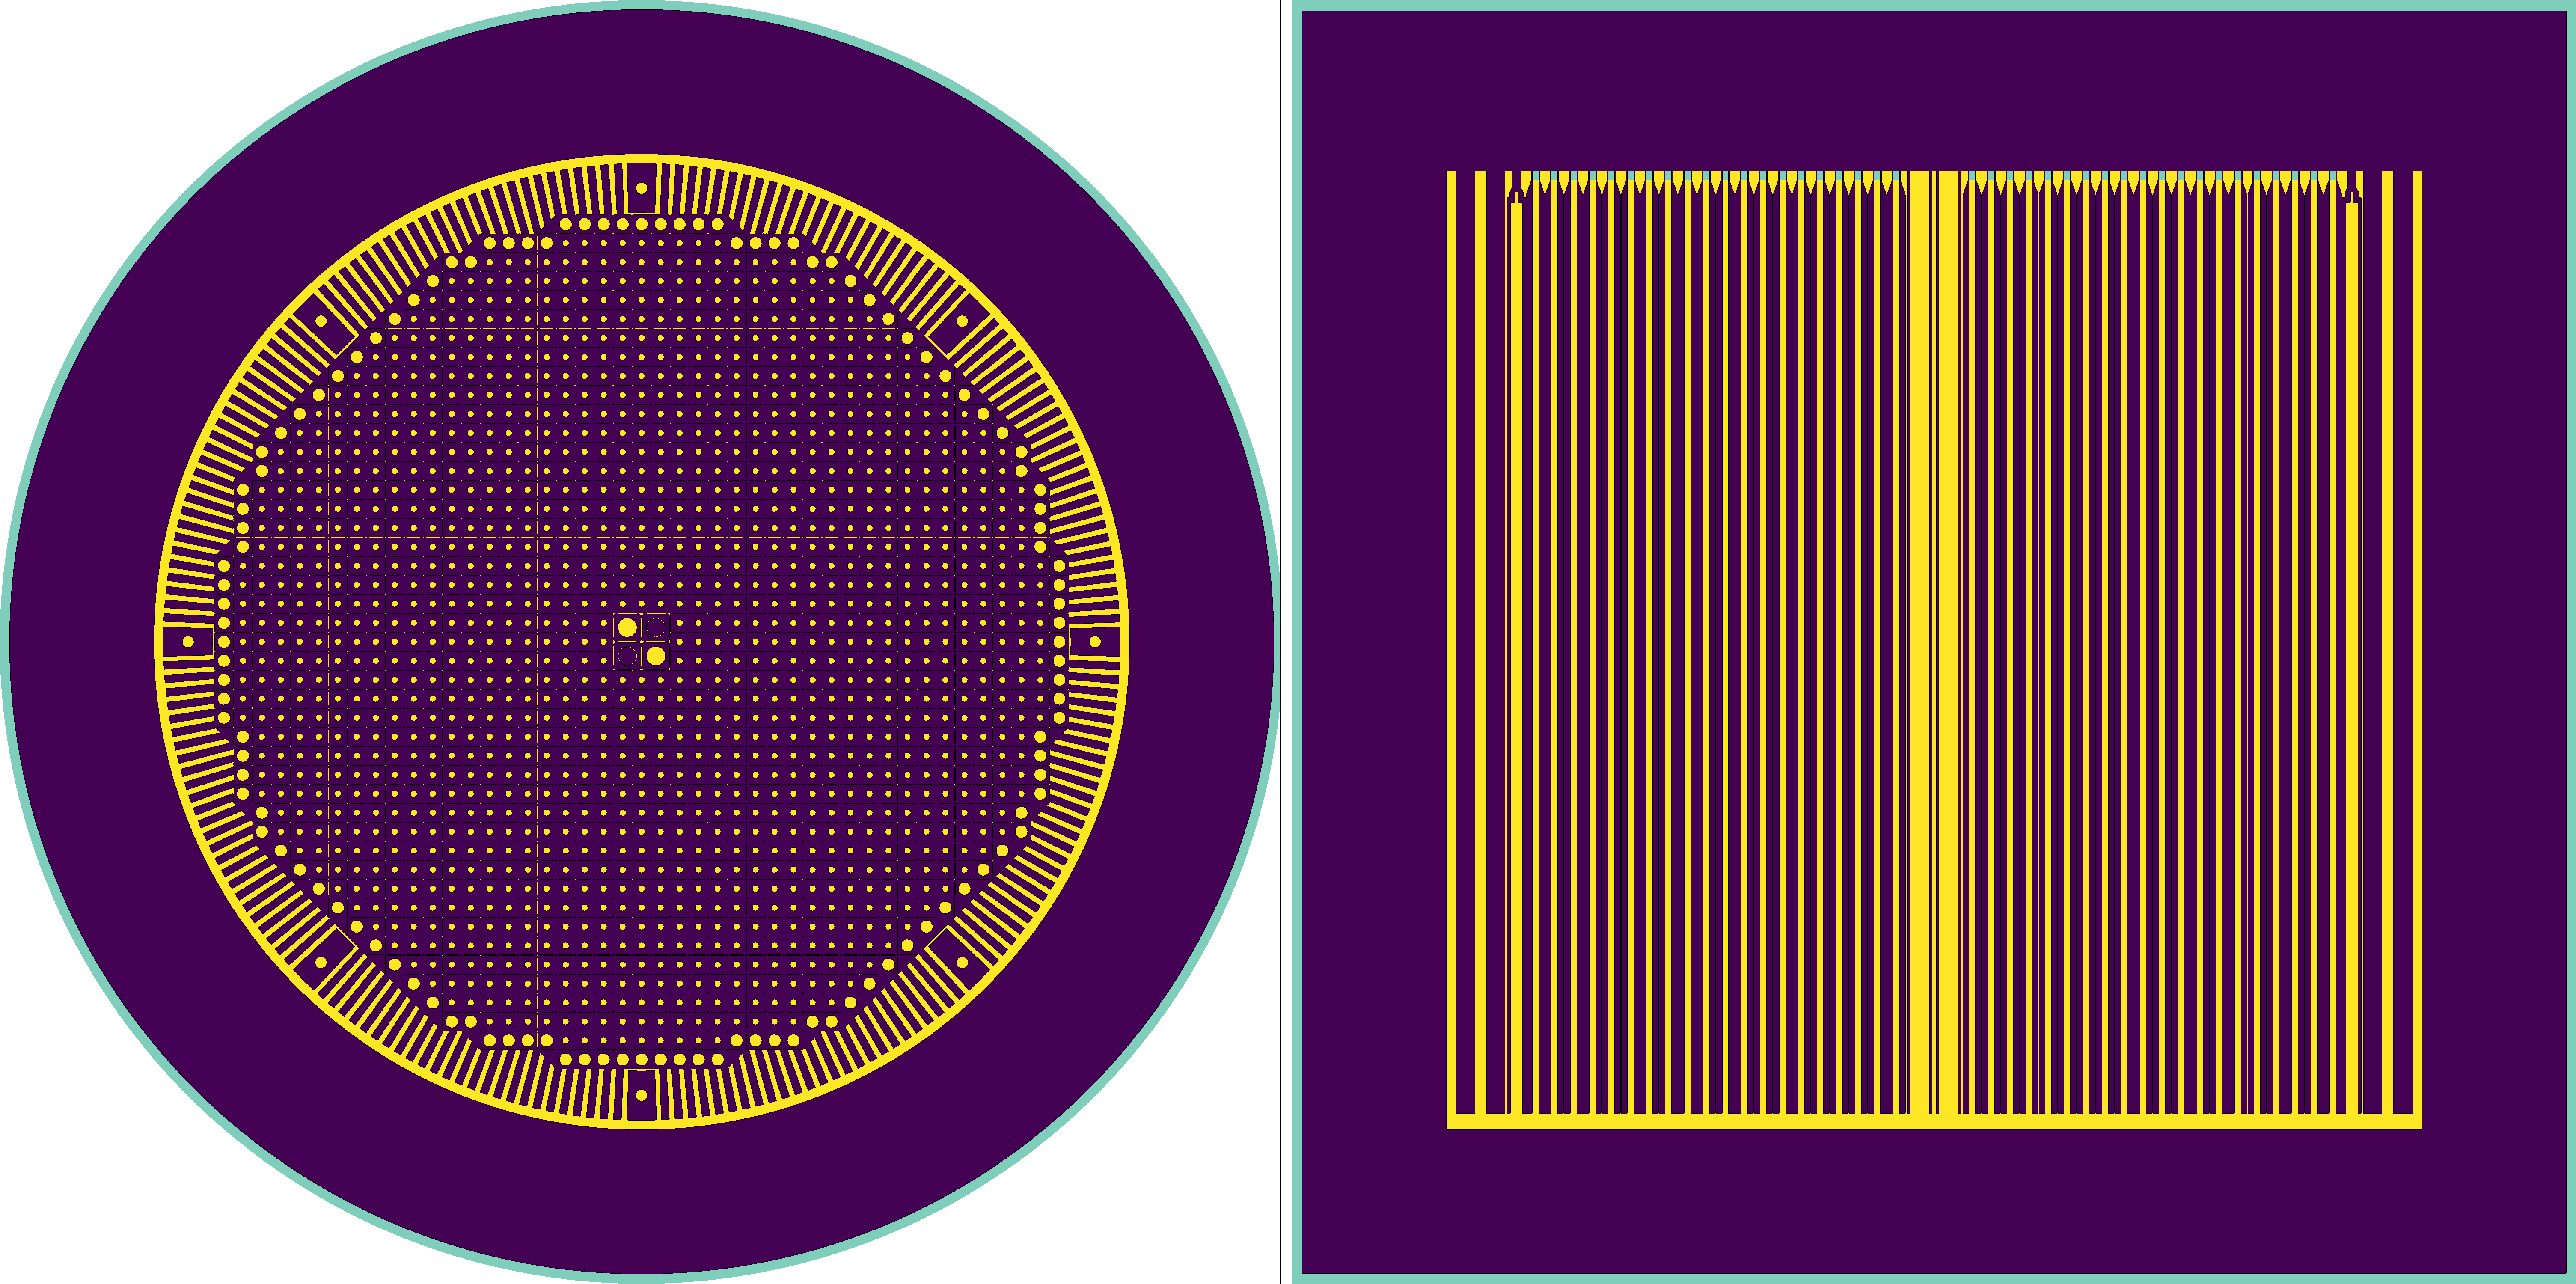
\includegraphics[width=\textwidth]{ch3/view_serpent.png}
	\caption{$XY$ (left) and $XZ$ (right) views of a Serpent \gls{MSBR} model 
	(reproduced from Rykhlevskii \emph{et al.} 
	\cite{rykhlevskii_modeling_2019}).}
	\label{fig:serpent_plan_view}
\end{figure}

\begin{figure}[t!] % replace 't' with 'b' to \centering
	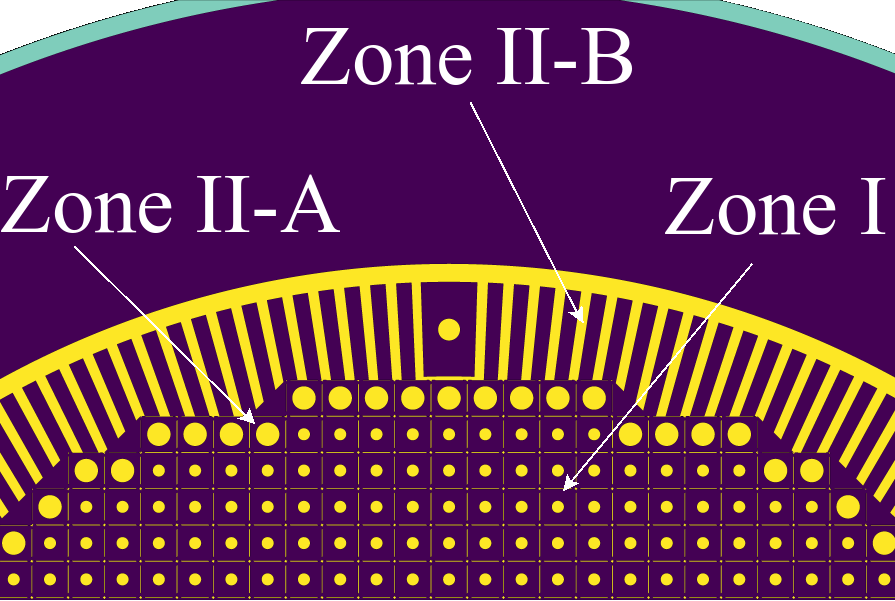
\includegraphics[width=\textwidth]{ch3/ser_zone_II.png}
	\caption{Detailed view of the \gls{MSBR} two-zone model. 
		Yellow represents fuel salt, purple represents graphite, and aqua 
		represents the reactor vessel (reproduced from Rykhlevskii 
		\emph{et al.} \cite{rykhlevskii_modeling_2019}).}
	\label{fig:serpent_zoneII}
\end{figure}

Since reactor graphite experiences significant dimensional changes due to 
neutron irradiation, the reactor core was designed for periodic replacement. 
Based on the experimental irradiation data from the \gls{MSRE}, the core 
graphite lifetime is about 4 years, and the reflector graphite lifetime is 30 
years \cite{robertson_conceptual_1971}.

The core design also has eight symmetric graphite slabs with a width of 15.24 
cm in zone II, one of which is illustrated in Figure~\ref{fig:serpent_zoneII}. 
The holes in the centers are for the core lifting rods used during the core 
replacement operations. These holes also allow a portion of the fuel salt to 
flow to the top of the vessel for cooling the top head and axial reflector.  
Figure~\ref{fig:serpent_zoneII} also shows the 5.08-cm-wide annular 
space between the removable core graphite in zone II-B and the permanently 
mounted reflector graphite. This annulus consists entirely of fuel salt, 
provides space for moving the core assembly, helps compensate for the 
elliptical dimensions of the reactor vessel, and serves to reduce the damaging 
flux at the surface of the graphite reflector blocks. 

$^{135}$Xe is a strong neutron poison, and some fraction of this gas is  
absorbed by graphite during \gls{MSBR} operation. ORNL calculations showed 
that for unsealed commercial graphite with a helium permeability of 10$^{-5}$ 
cm$^2$/s, the calculated poison fraction is less than 2\% 
\cite{robertson_conceptual_1971}. This parameter can be improved by using 
experimental graphite types or by applying sealing technology. The effect of 
the gradual poisoning of the core graphite with xenon is out of the scope if 
this work.

\subsection{Core zone I}
The central region of the core, called zone I, is made up of graphite 
elements, each $10.16$cm$\times$ 10.16cm$\times$396.24cm. Zone I has 4 
channels for control rods: two for graphite rods, which both regulate and shim 
during normal operation, and two for backup safety rods consisting of boron 
carbide clad to assure sufficient negative reactivity for accidents.

These graphite elements have a mostly rectangular shape with lengthwise ridges 
at each corner that leave space for salt flow elements. Various element sizes 
reduce the peak damage flux and power density in the center of the core to 
prevent local graphite damage. Figure~\ref{fig:I_element_ref} shows the 
elevation and plan views of graphite elements of zone I 
\cite{robertson_conceptual_1971} and their Serpent model 
\cite{rykhlevskii_full-core_2017}.
\begin{figure}[ht!] % replace 't' with 'b' to \centering
	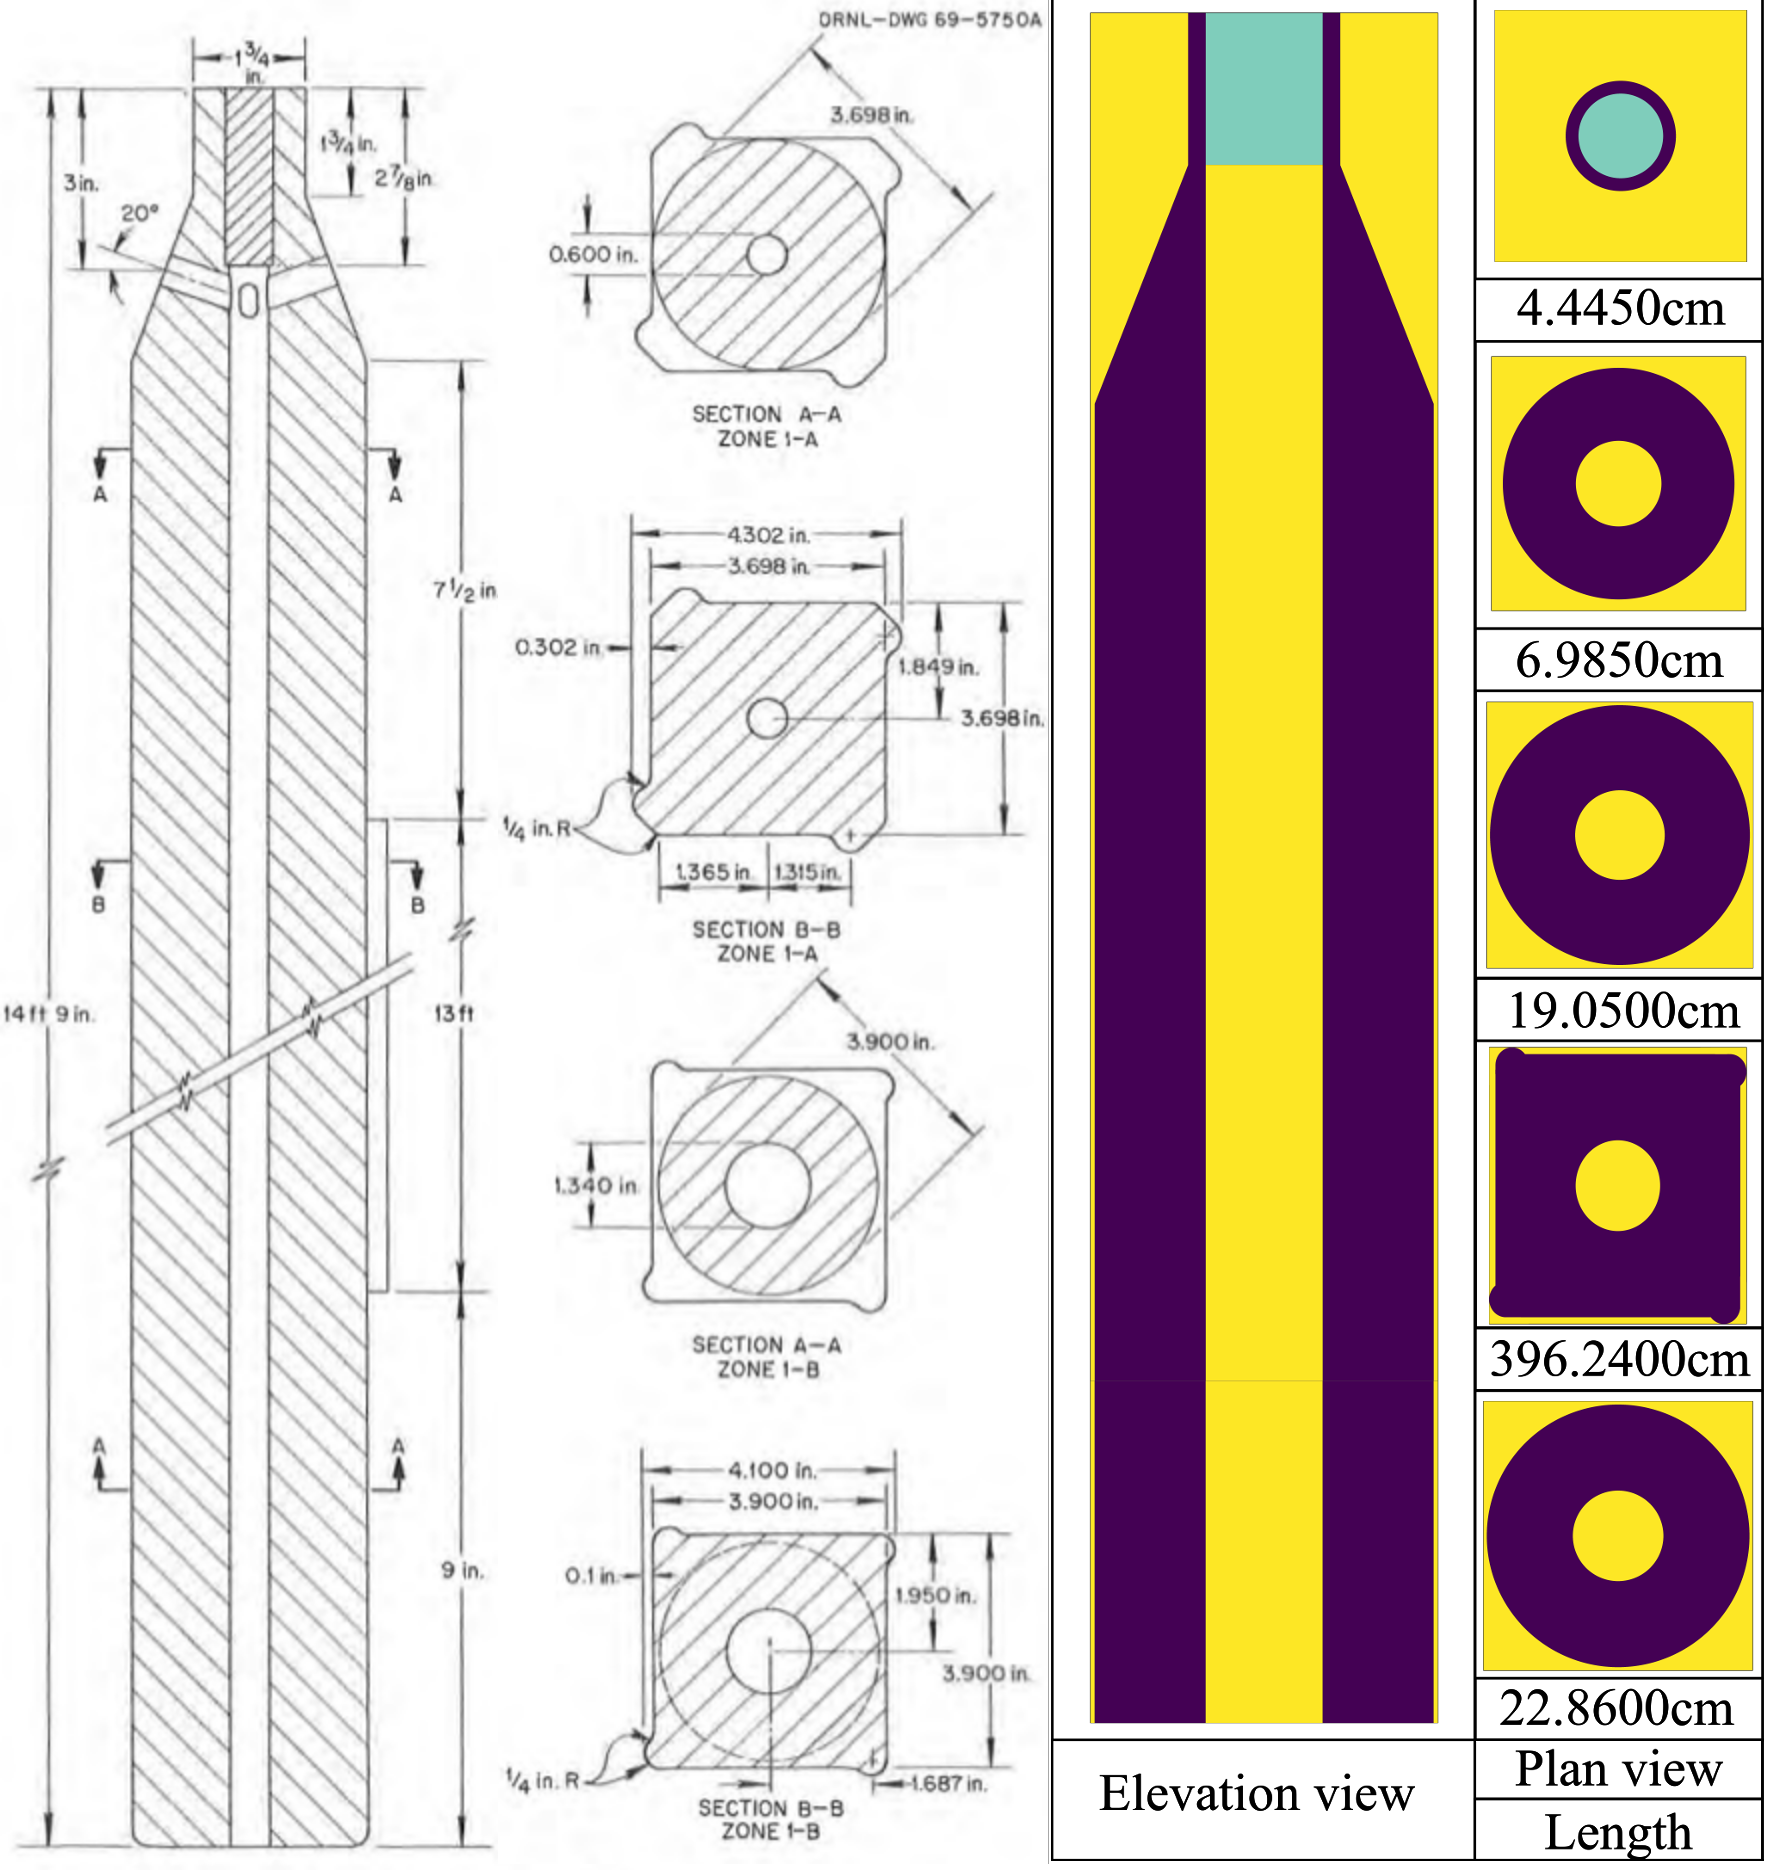
\includegraphics[width=\textwidth]{ch3/zone_I_element_ref.png}
	\caption{Graphite moderator elements for zone I: reference design (left)
		\cite{robertson_conceptual_1971} and Serpent model (right) 
		\cite{rykhlevskii_full-core_2017}.  Yellow 
		represents fuel salt, purple represents graphite, and aqua represents 
		the reactor vessel ()reproduced from Rykhlevskii \emph{et al.} 
		\cite{rykhlevskii_modeling_2019}).}
	\label{fig:I_element_ref}
\end{figure}

\subsection{Core zone II}
Zone II, which is undermoderated, surrounds zone I. Combined with the bounding 
radial reflector, zone II serves to diminish neutron leakage. Two kinds of 
elements form this zone: large-diameter fuel channels (zone II-A) and 
radial graphite slats (zone II-B). 

Zone II has 37\% fuel salt by volume, and each element has a fuel channel 
diameter of 6.604cm. The graphite elements for zone II-A are prismatic, with
elliptical dowels running axially between the prisms. These dowels
isolate the fuel salt flow in zone I from that in zone II.  
Figure~\ref{fig:II_element_ref} shows the shapes and dimensions of these 
graphite elements and their Serpent model. Zone II-B elements are rectangular 
slats spaced far enough apart to provide the 0.37 fuel salt volume fraction. 
The reactor zone II-B graphite 5.08cm-thick slats vary in the radial dimension 
(average width is 26.67cm) as shown in Figure~\ref{fig:serpent_zoneII}. Zone 
II serves as a blanket to achieve the best performance: a high breeding ratio 
and a low fissile inventory. The harder neutron energy spectrum in zone II 
enhances the rate of thorium resonance capture relative to the fission rate, 
thus limiting the neutron flux in the outer core zone and reducing the neutron 
leakage \cite{robertson_conceptual_1971}. 

The sophisticated, irregular shapes of the fuel elements challenge an accurate 
representation of zone II-B. The suggested design 
\cite{robertson_conceptual_1971} of zone II-B has eight irregularly-shaped 
graphite elements as well as dozens of salt channels. These graphite elements 
were simplified into right-circular cylindrical shapes with central channels. 
Figure~\ref{fig:serpent_zoneII} illustrates this core region in the Serpent 
model. The volume of fuel salt in zone II was kept exactly at 37\% so 
this simplification unaffected the core neutronics. 
Simplifying the eight edge channels was the only simplification made to the 
\gls{MSBR} geometry in this work. 
\begin{figure}[ht!] % replace 't' with 'b' to \centering
	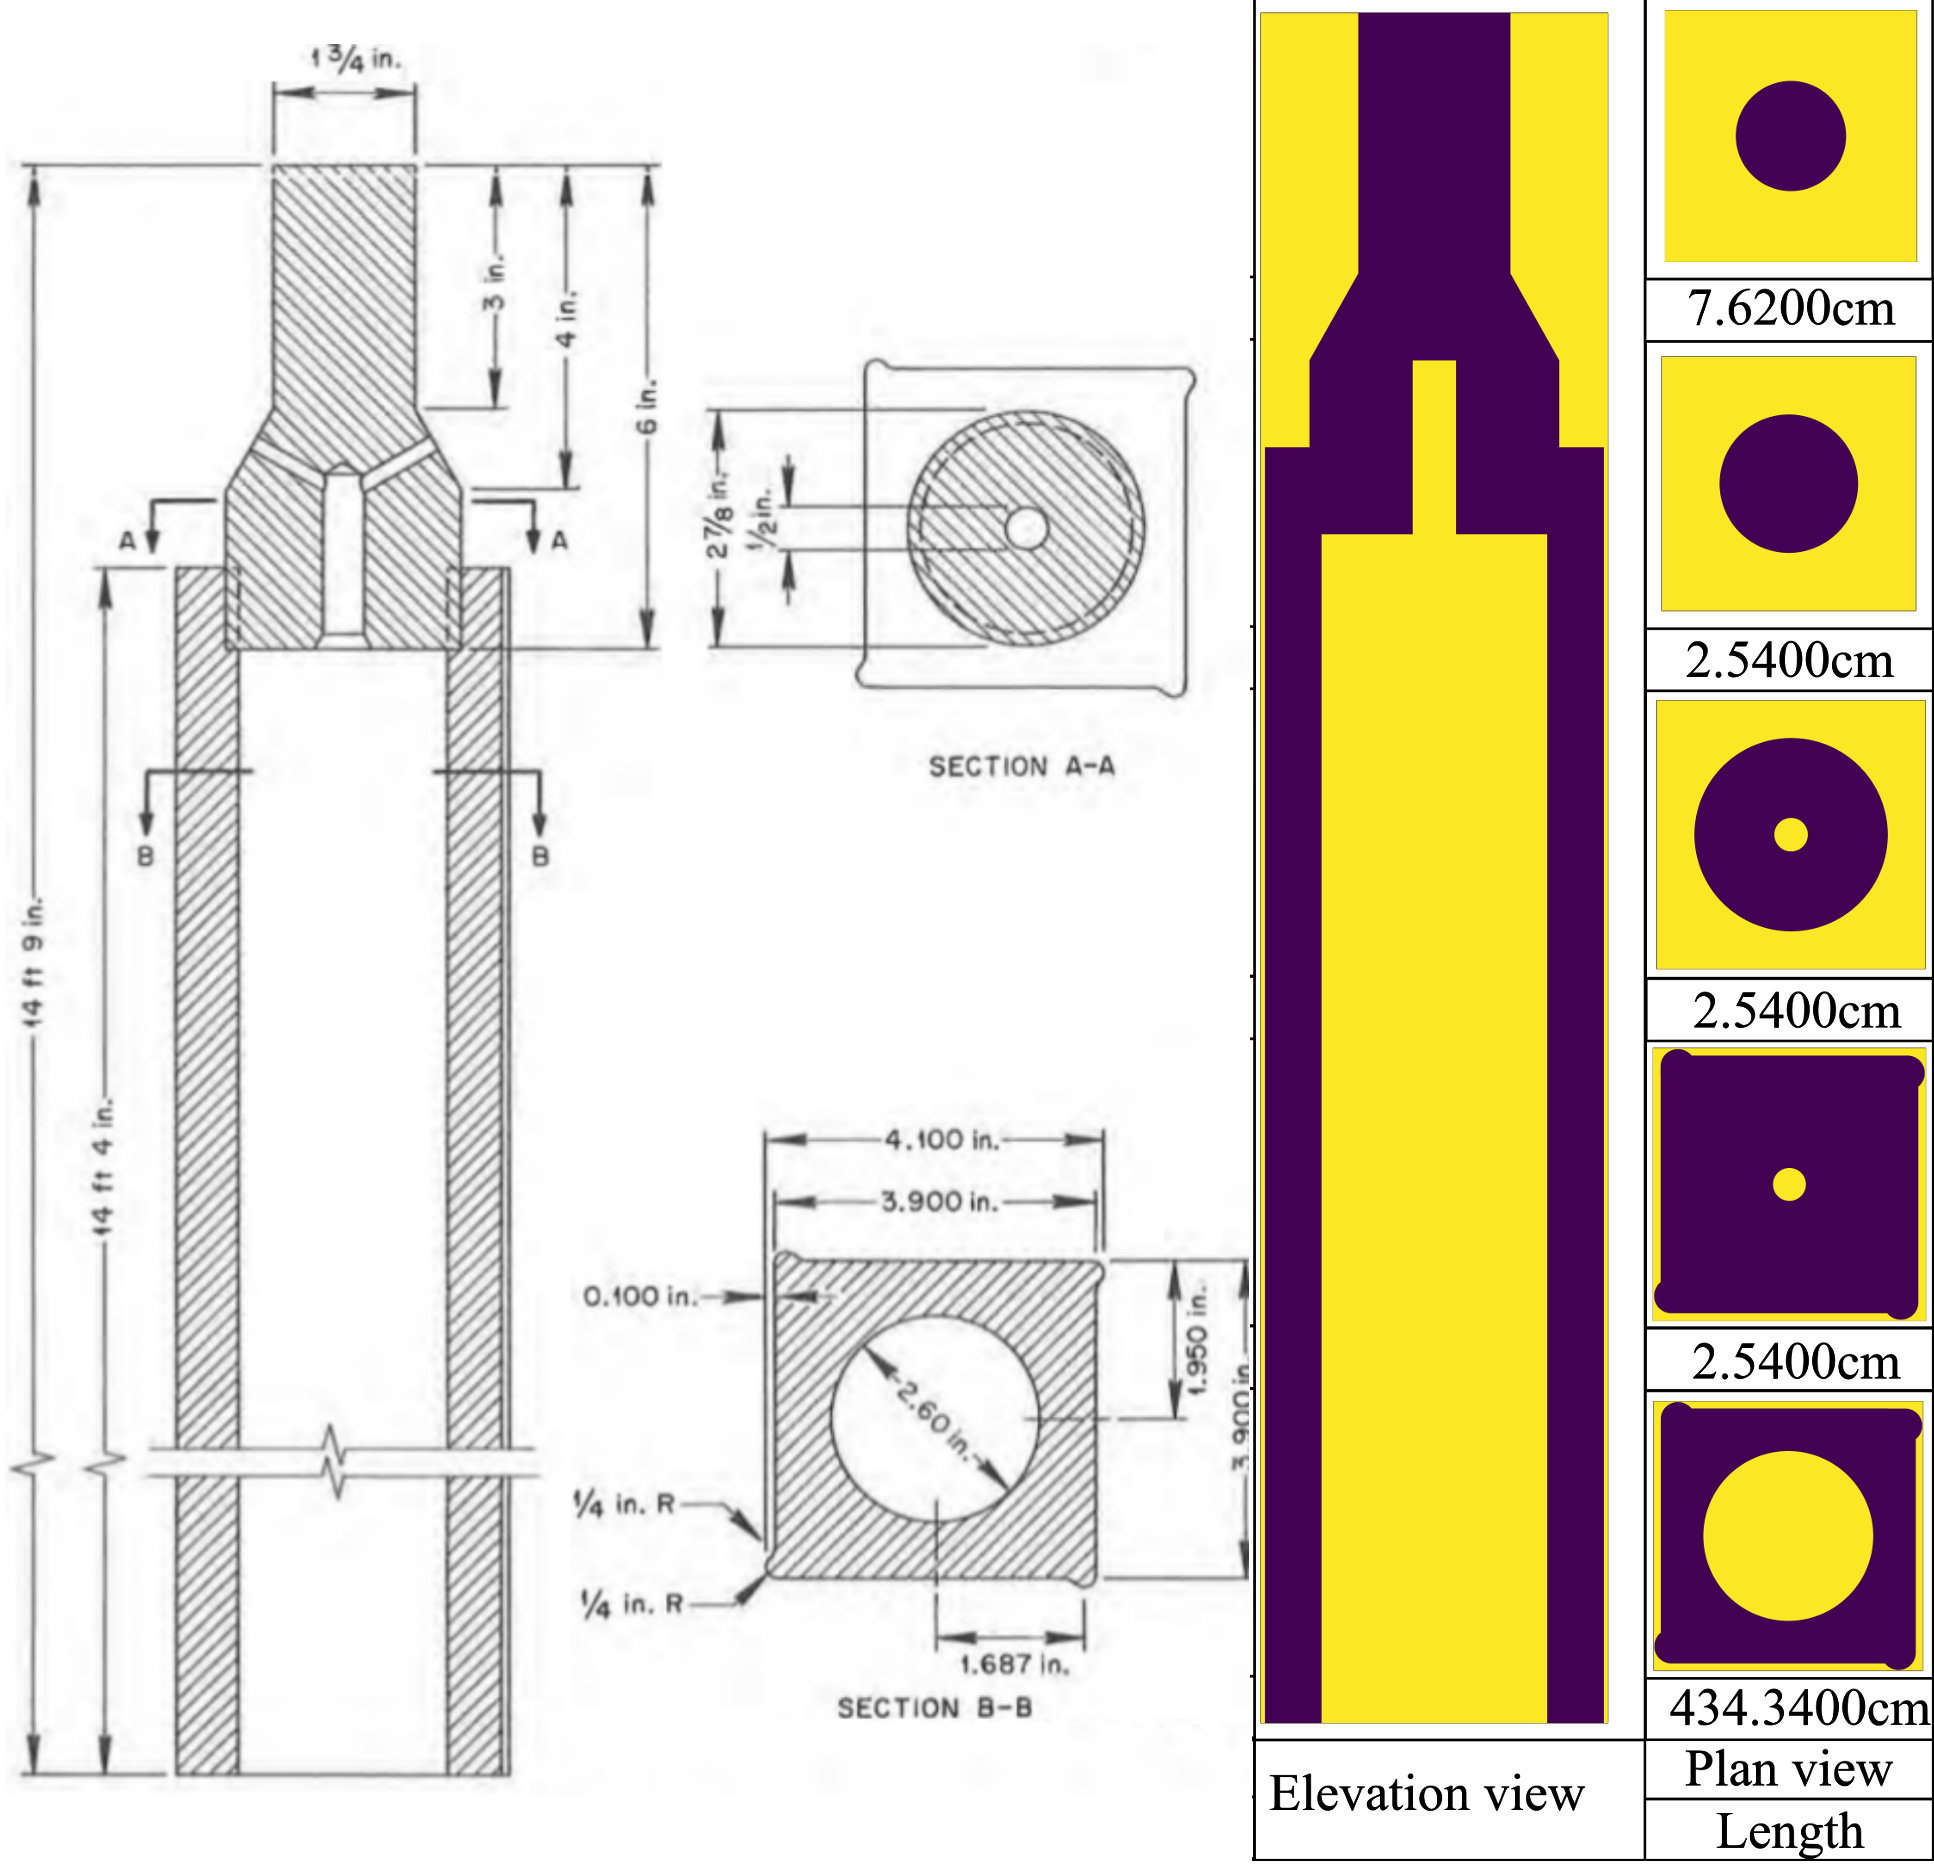
\includegraphics[width=\textwidth]{ch3/zone_II_element_ref.png}
	\caption{Graphite moderator elements for zone II-A: reference design (left)
		\cite{robertson_conceptual_1971} and Serpent model (right) 
		\cite{rykhlevskii_full-core_2017}.  Yellow 
		represents fuel salt, purple represents graphite, and aqua represents 
		the reactor vessel (reproduced from Rykhlevskii \emph{et al.} 
		\cite{rykhlevskii_modeling_2019}).}
	\label{fig:II_element_ref}
\end{figure}

\subsection{Material composition and normalization parameters}
The fuel salt, reactor graphite, and modified Hastelloy-N are all materials 
created at \gls{ORNL} specifically for the \gls{MSBR}. The initial fuel salt 
used the same density (3.35 g/cm$^3$) and composition  
LiF-BeF$_2$-ThF$_4$-$^{233}$UF$_4$ (71.75-16-12-0.25 mole \%) as the 
\gls{MSBR} design \cite{robertson_conceptual_1971}. The lithium in the molten 
salt fuel is fully enriched to 100\% $^{7}$Li because $^{6}$Li is an extremely 
strong neutron poison and becomes tritium upon neutron capture. 

The specific temperature was fixed for each material and stays constant during 
the reactor operation. The isotopic composition of each material at the 
initial state was described in detail in the MSBR conceptual design study 
\cite{robertson_conceptual_1971} and has been applied to the Serpent model 
without any modification. Table~\ref{tab:msbr_tab} is a summary of the major 
\gls{MSBR} parameters used to inform the Serpent model  
\cite{robertson_conceptual_1971}. 
%%%%%%%%%%%%%%%%%%%%%%%%%%%%%%%%%%%%%%%%
\begin{table}[h!]
	\caption{Summary of principal data for the \gls{MSBR} (reproduced from 
	Robertson \emph{et al.} \cite{robertson_conceptual_1971}).}
	\begin{tabularx}{\textwidth}{ X  X}
		\hline
		Thermal power           					& 2250 MW$_{th}$\\
		Electric power             					& 1000 MW$_e$   \\
		Gross thermal efficiency       				& 44.4\%        \\
		Salt volume fraction in central zone I		& 0.13   		\\
		Salt volume fraction in outer zone II       & 0.37			\\
		Fuel salt inventory (Zone I)                & 8.2 m$^3$		\\
		Fuel salt inventory (Zone II)               & 10.8 m$^3$	\\
		Fuel salt inventory (annulus)               & 3.8 m$^3$		\\
		Total fuel salt inventory                   & 48.7 m$^3$	\\
		Fissile mass in fuel salt                   & 1303.7 kg		\\
		Fuel salt components   	& LiF-BeF$_2$-ThF$_4$-$^{233}$UF$_4$\\  
		Fuel salt composition   & 71.75-16-12-0.25 mole\%			\\
		Fuel salt density       & 3.35 g/cm$^3$         			\\ \hline
	\end{tabularx}
	\label{tab:msbr_tab}
\end{table}
%%%%%%%%%%%%%%%%%%%%%%%%%%%%%%%%%%%%%%%%%%%%%%%%

As mentioned in section~\ref{sec:reproc-plant}, the \gls{MSBR} design 
requires online reprocessing to remove neutron gaseous \glspl{FP} (Xe, Kr) and 
noble metals (e.g., Se, Nb, and Mo) every 20 seconds.  The $^{232}$Th in the 
fuel absorbs thermal neutrons and produces $^{233}$Pa, which then decays into 
the fissile $^{233}$U. Protactinium presents a challenge since it has a large 
absorption cross section in the thermal energy spectrum. Moreover, $^{233}$Pa 
left in the core would produce $^{234}$Pa and $^{234}$U, neither of which are 
useful as fuel. Accordingly, $^{233}$Pa is continuously removed from the fuel 
salt into a protactinium decay tank to allow $^{233}$Pa to decay to $^{233}$U 
without the corresponding negative neutronic impact. The reactor chemical 
processing system must separate $^{233}$Pa from the molten salt fuel over 3 
days, hold it while $^{233}$Pa decays into $^{233}$U, and return it to 
the primary loop. This feature allows the reactor to avoid neutron losses to 
protactinium, lowers in-core fission product inventory, and increases the 
efficiency of $^{233}$U breeding.

Table~\ref{tab:reprocessing_list_msbr} summarizes a full list of nuclides and 
their cycle time used for modeling salt treatment and separations 
\cite{robertson_conceptual_1971}. The removal rates vary among chemical 
elements in this reactor concept and dictate the necessary resolution of 
depletion calculations. If the depletion time intervals are short, an 
enormous number of depletion steps are required to obtain the equilibrium 
composition. On the other hand, if the depletion  calculation time interval is 
too long, the impact of short-lived fission products is not captured. To 
compromise, a 3-day time interval was selected for depletion calculations to 
correlate with the removal interval of $^{233}$Pa, and $^{232}$Th was 
continuously added to maintain the initial mass fraction of $^{232}$Th.
%%%%%%%%%%%%%%%%%%%%%%%%%%%%%%%%%%%%%%%%
\begin{table}[ht!]
	\caption{The cycle times for protactinium and fission 
		products removal from the \gls{MSBR} (reproduced from Robertson 
		\emph{et al.} 
		\cite{robertson_conceptual_1971}).}
	\begin{tabularx}{\textwidth}{x  s  x}
		\hline \textbf{Processing group} & \qquad\qquad\qquad 
		\textbf{Nuclides} & \textbf{Cycle time (at full power)} \\ \hline 
		Rare earths & Y, La, Ce, Pr, Nd, Pm, Sm, 
		Gd & 50 days \\ \qquad & Eu & 500 days \\ Noble metals & Se, 
		Nb, Mo, Tc, Ru, Rh, Pd, Ag, Sb, Te & 20 sec \\
		Semi-noble metals & Zr, Cd, In, Sn & 200 days \\
		Gases & Kr, Xe & 20 sec \\ Volatile fluorides & Br, I & 60 days \\
		Discard & Rb, Sr, Cs, Ba & 3435 days \\ 
		%Salt discard & Th, Li, Be, F & 3435 days \\ 
		Protactinium & $^{233}$Pa & 3 days \\ Higher 
		nuclides & $^{237}$Np, $^{242}$Pu & 16 years \\  \hline
	\end{tabularx}
	\label{tab:reprocessing_list_msbr}
\end{table}
%%%%%%%%%%%%%%%%%%%%%%%%%%%%%%%%%%%%%%%%%

\section{Fuel salt isotopic composition dynamics and equilibrium search}
\label{sec:equilibrium_search}
The SaltProc online reprocessing simulation package is demonstrated in four 
applications: 
(1) analyzing the \gls{MSBR} neutronics and fuel cycle to find 
the equilibrium core composition and fuel salt depletion, 
(2) demonstrating that in a single-fluid two-region \gls{MSBR} conceptual 
design the undermoderated outer core zone II works as a virtual ``blanket'', 
reduces neutron leakage, and improves breeding ratio due to neutron energy 
spectral shift,
(3) studying operational and safety parameters evolution during \gls{MSBR} 
operation, and
(4) determining the effect of fission product removal on the core neutronics. 
This section discusses the first two applications.

The neutron population per cycle and the number of active/inactive cycles were 
chosen to compromise between reasonable uncertainty for a transport 
problem ($\leq$ 15 pcm\footnote{ $1$ $pcm$ = 10$^{-5}\Delta k_{eff}/k_{eff}$} 
for effective multiplication factor) and computational time. The \gls{MSBR} 
depletion and safety parameter computations were performed on 64 Blue Waters 
XK7 nodes (two AMD 6276 Interlagos CPU per node, 16 floating-point Bulldozer 
core units per node or 32 ``integer'' cores per node, nominal clock speed is 
2.45 GHz). The total computational time for calculating fuel salt depletion  
during 60 years of operation was approximately 9,900 node-hours (18 
core-years.)

\subsection{Effective multiplication factor dynamics}
Figures~\ref{fig:keff} and \ref{fig:keff_zoomed} show the effective 
multiplication factors obtained using SaltProc v0.1 and Serpent. The effective 
multiplication factors were calculated after removing fission products listed 
in Table~\ref{tab:reprocessing_list_msbr} and adding the fertile material at 
the end of each depletion step (3 days). The effective multiplication factor 
fluctuates significantly as a result of the batch-wise nature of this online 
reprocessing strategy. 
\begin{figure}[ht!] 
	\centering
	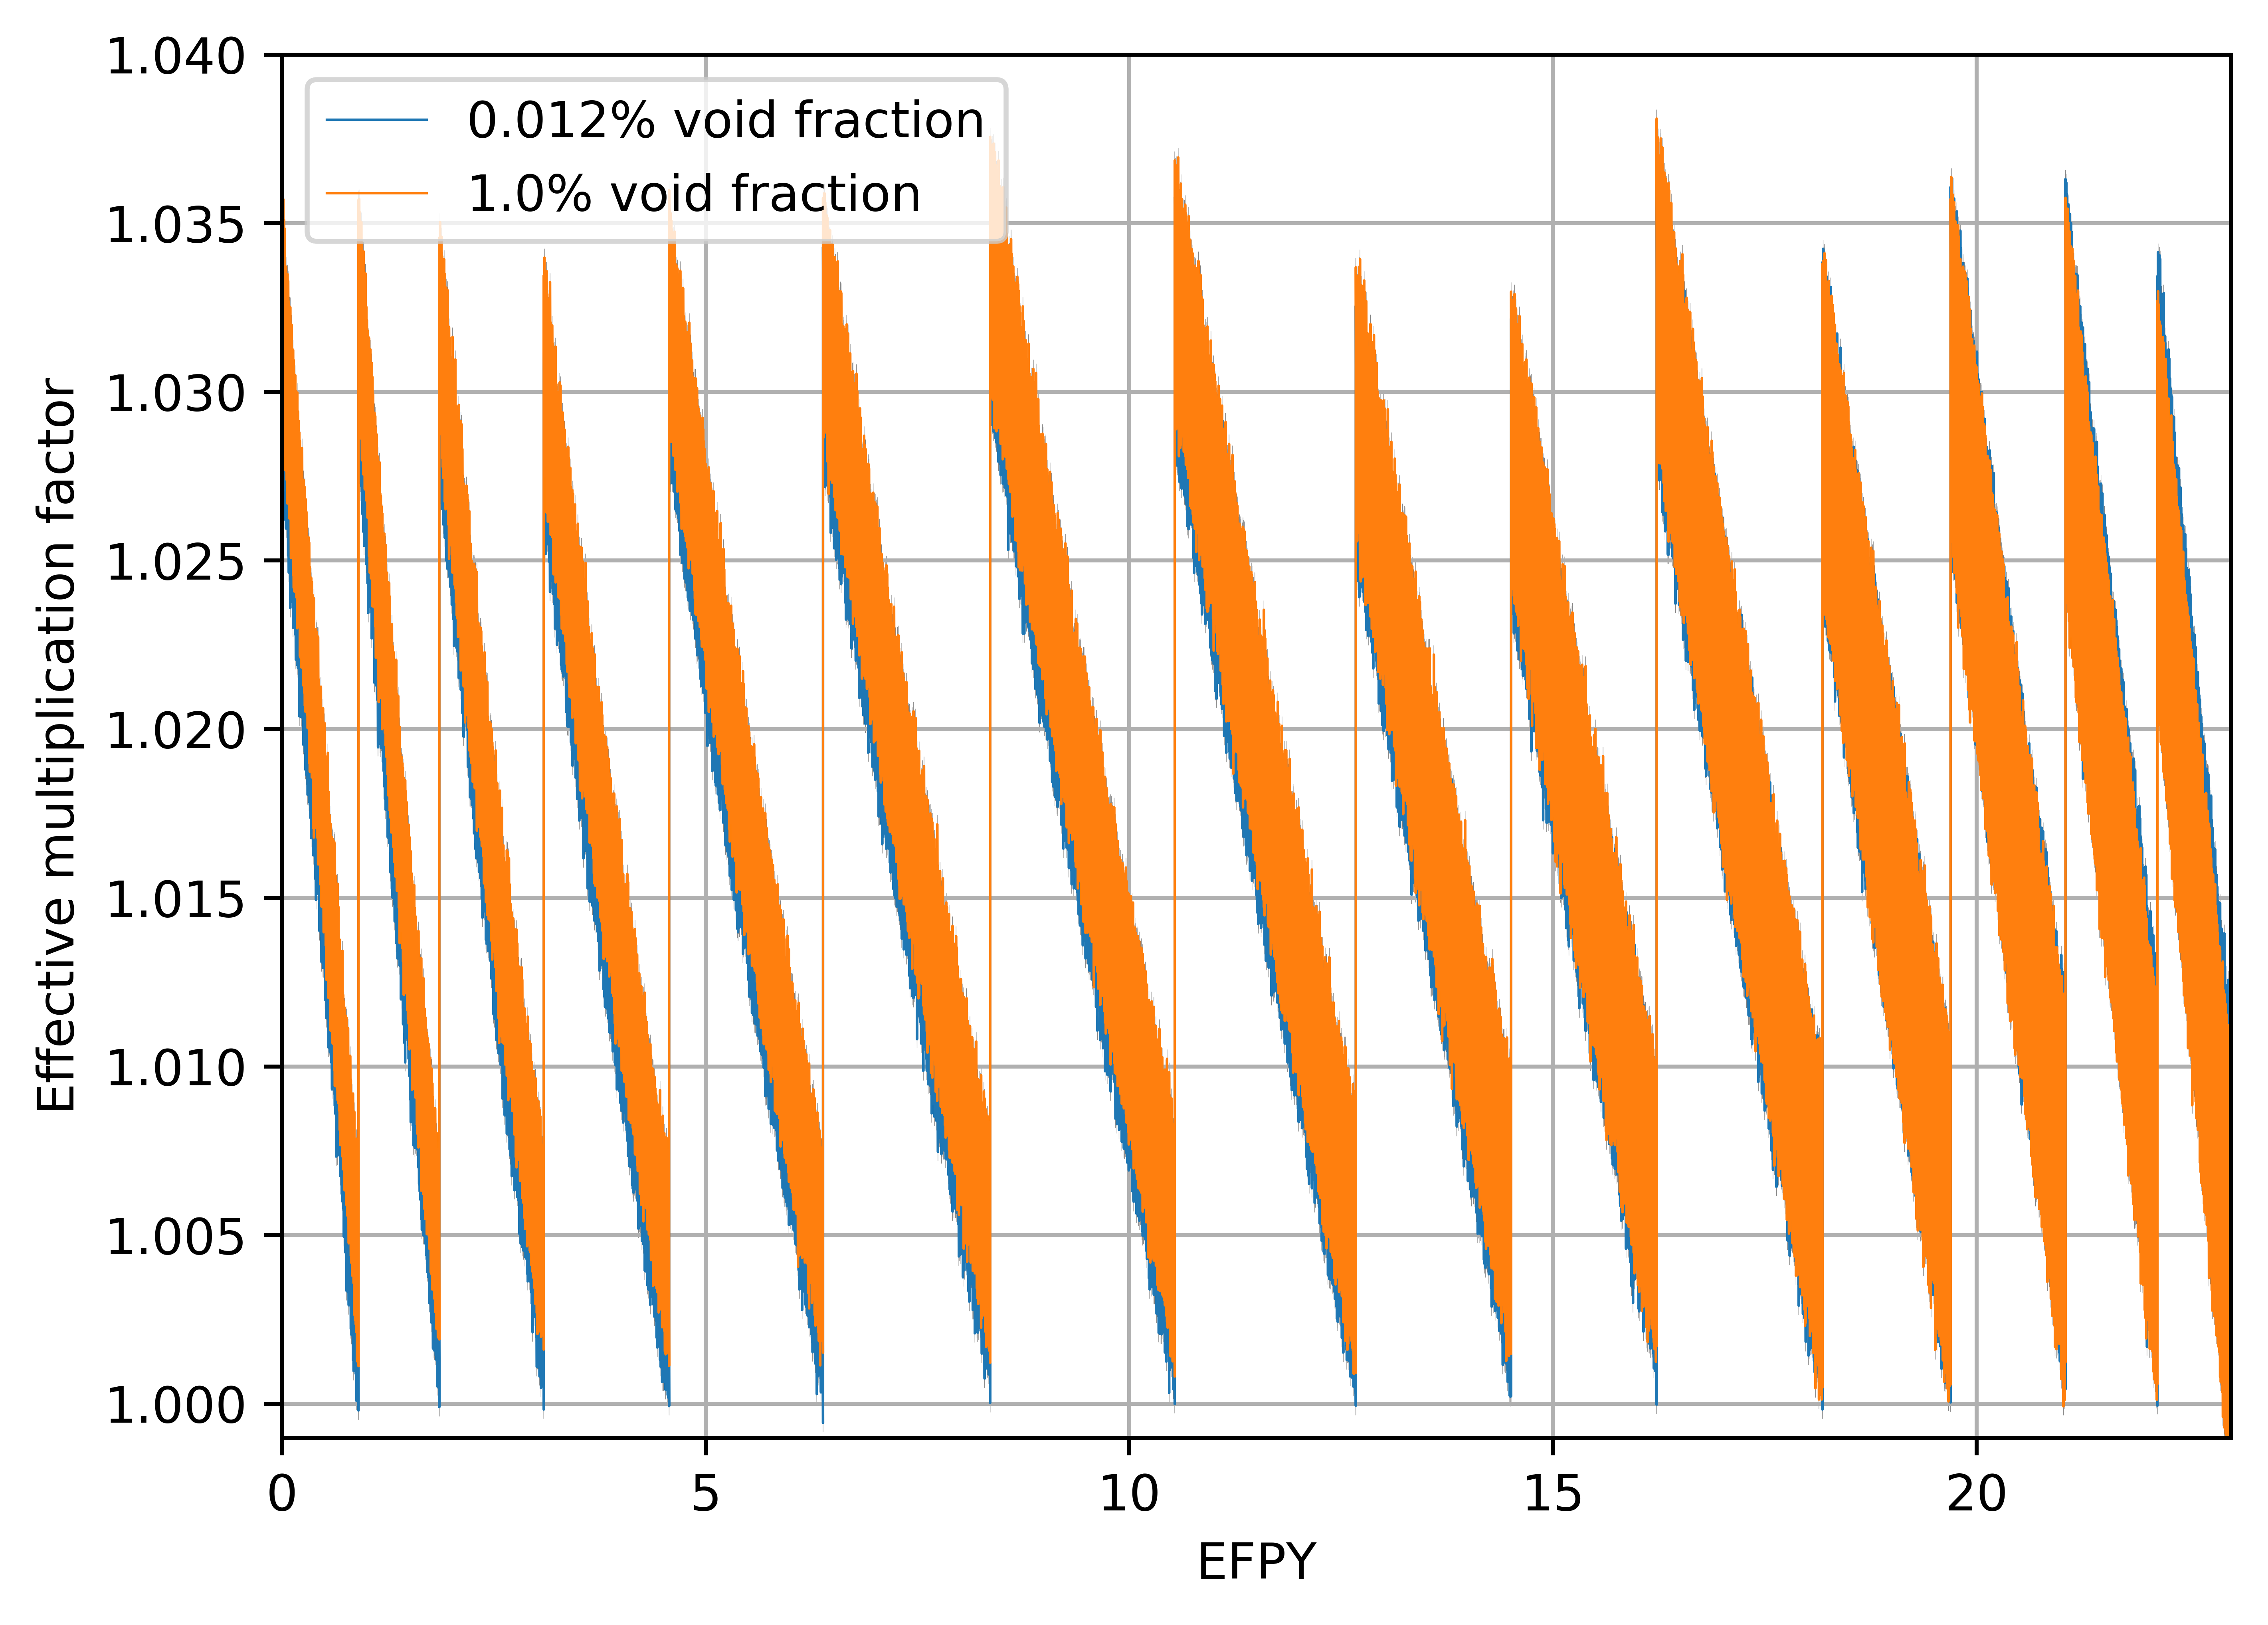
\includegraphics[width=\textwidth]{ch3/keff.png}
	\caption{Effective multiplication factor dynamics for full-core \gls{MSBR} 
		model over a 60-year reactor operation lifetime (reproduced 
		from Rykhlevskii \emph{et al.} \cite{rykhlevskii_modeling_2019}).}
	\label{fig:keff}
\end{figure}
\begin{figure}[ht!] 
	\centering
	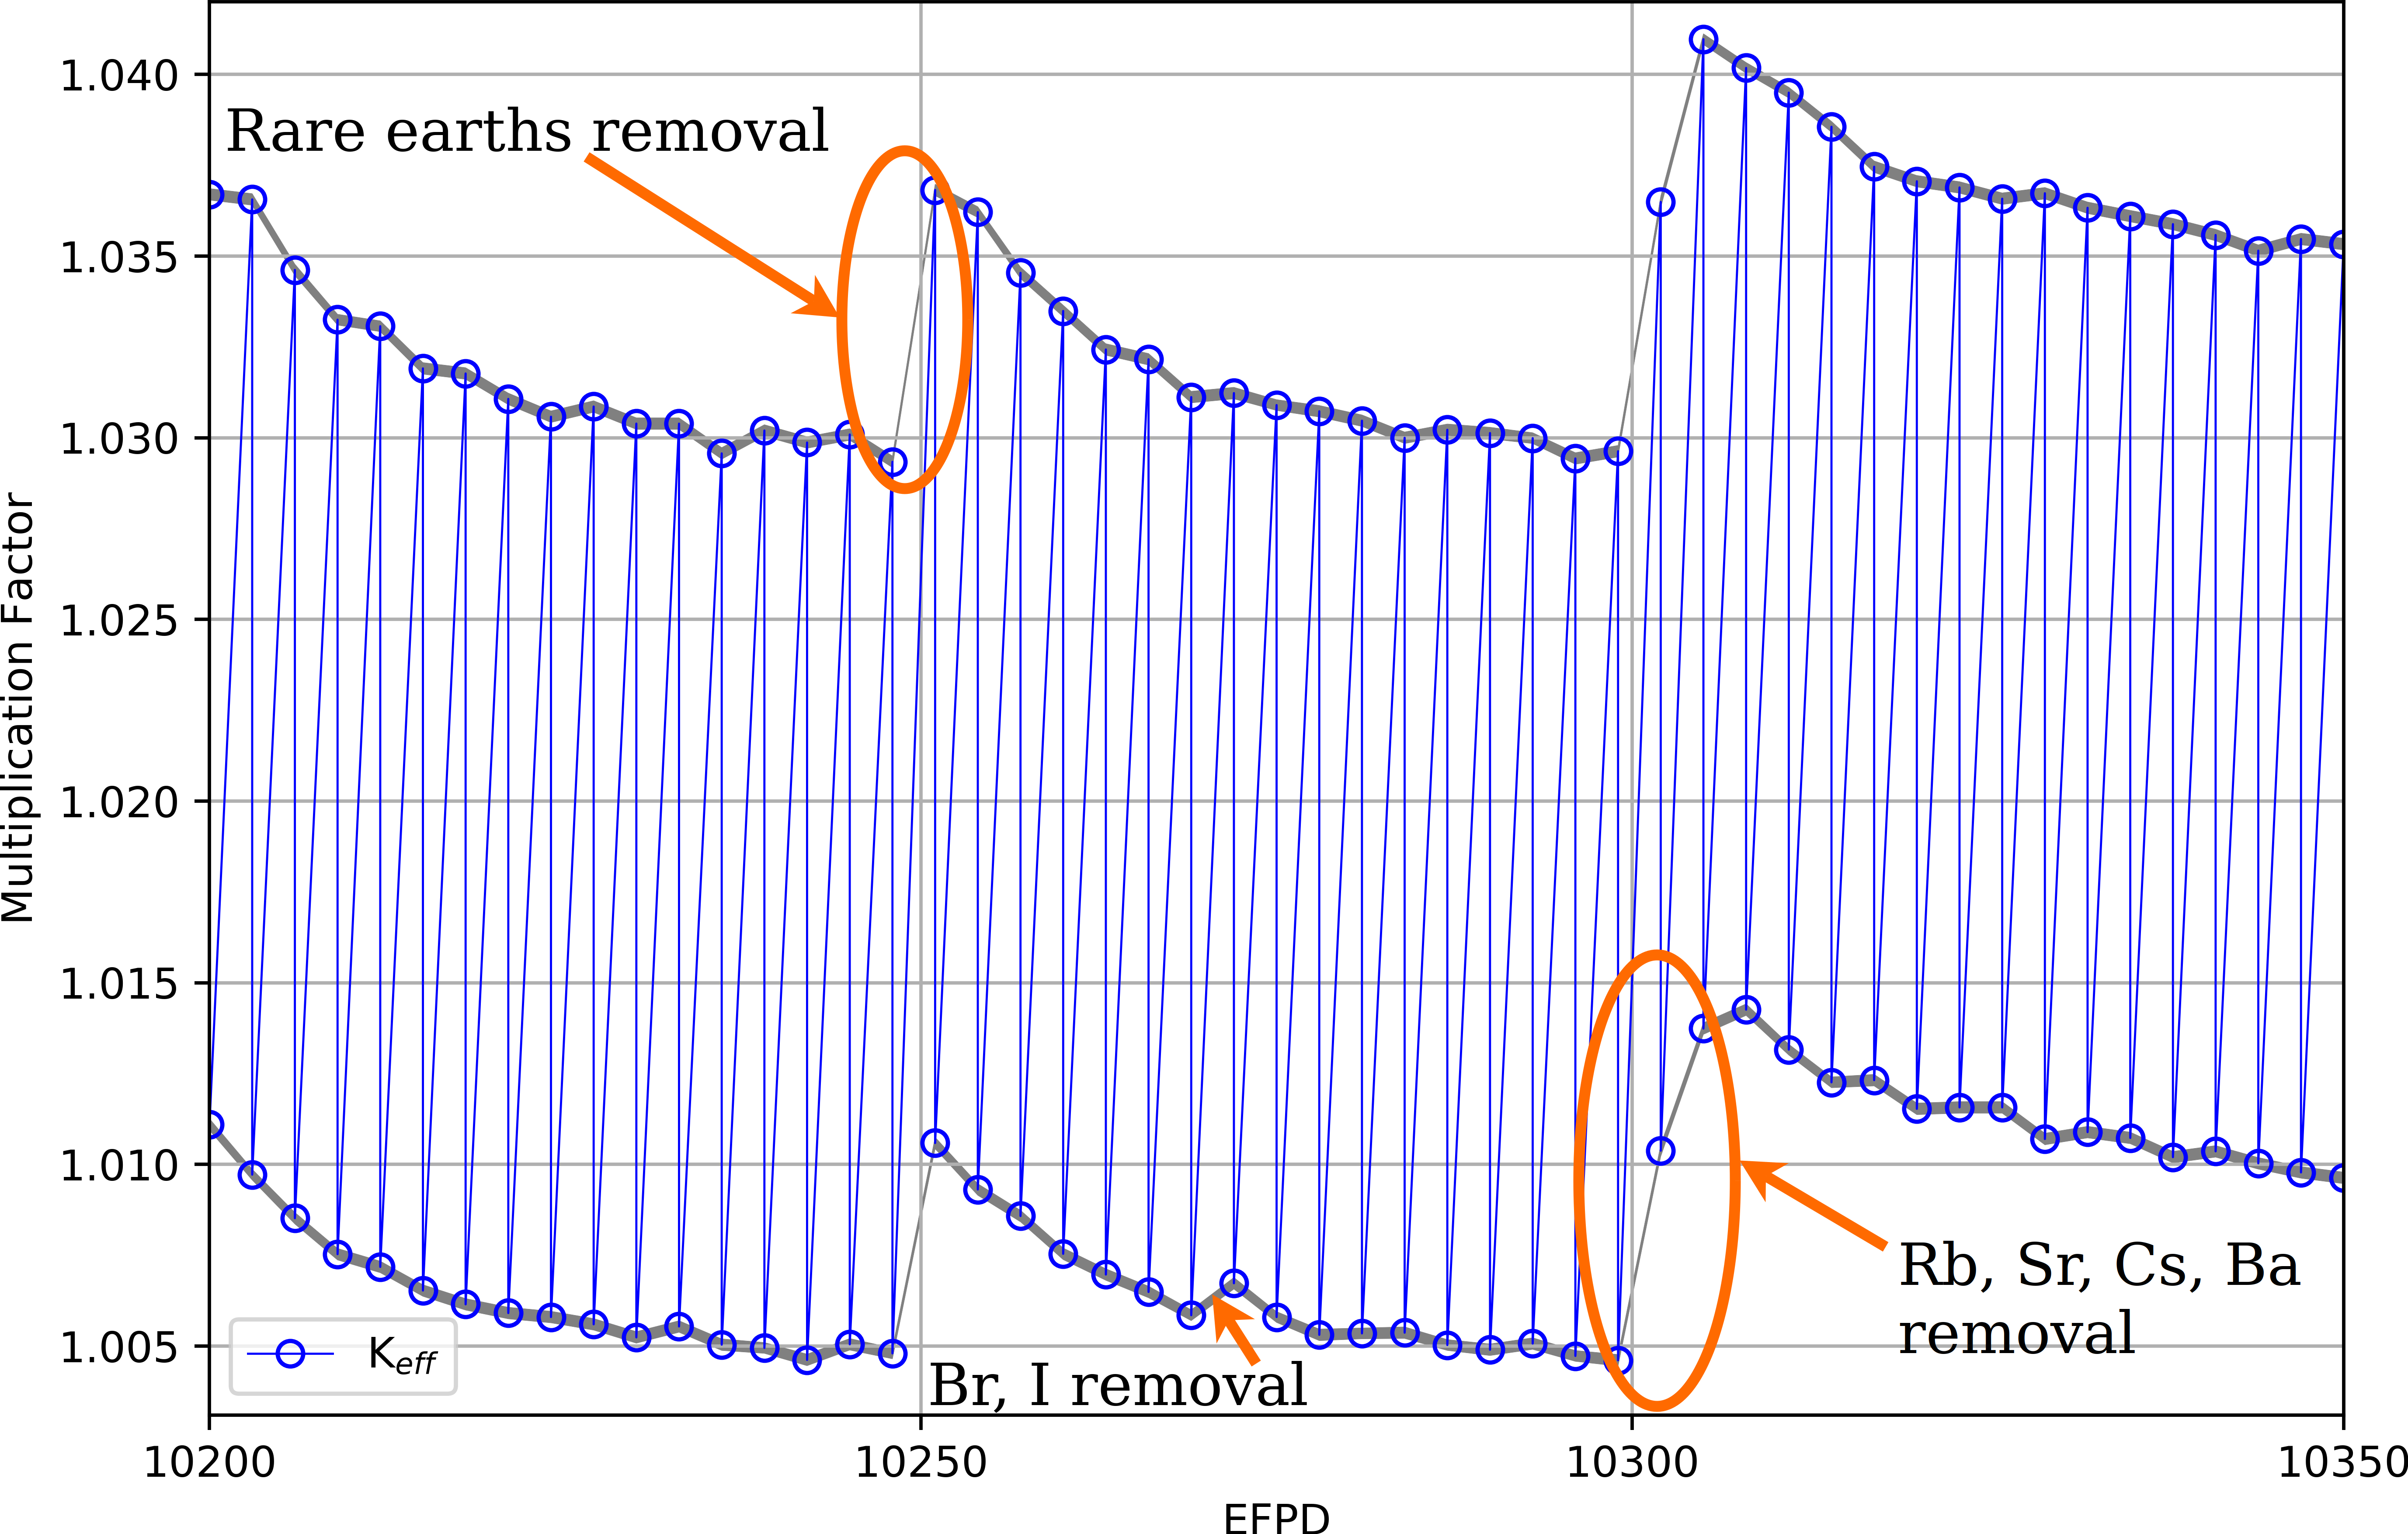
\includegraphics[width=\textwidth]{ch3/keff_zoomed.png}
	\caption{Zoomed effective multiplication factor for a 150-EFPD time 
	interval (reproduced from Rykhlevskii \emph{et al.}  
	\cite{rykhlevskii_modeling_2019}).}
	\label{fig:keff_zoomed}
\end{figure}

First, Serpent calculates the effective multiplication factor for the  
beginning of the cycle. 
Next, it computes the new fuel salt composition at the end of a 3-day 
depletion. The corresponding effective multiplication factor is much smaller 
than the previous one. Finally, Serpent calculates $k_{eff}$ for the depleted 
composition after applying feeds and removals. The $k_{eff}$ increases 
accordingly since major reactor poisons (e.g., Xe, Kr) are removed, while 
fresh fissile material ($^{233}$U) from the protactinium decay tank is added.  

Additionally, the presence of rubidium, strontium, cesium, and barium in the 
core are disadvantageous to reactor physics. Overall, the effective 
multiplication factor gradually decreases from 1.075 to $\approx$1.02 at 
equilibrium after approximately 6 years of irradiation. 

%In fact, SaltProc v0.1 fully removes all of these elements every 3435 days 
%(not a small mass fraction every 3 days) which causes the multiplication 
%factor to jump by approximately $450$ $pcm$, and limits using the batch 
%approach for online reprocessing simulations. In SaltProc v1.0 this drawback 
%has been eliminated by removing fraction of element at each depletion step 
%with 
%longer residence times (seminoble metals, volatile fluorides, Rb, Sr, Cs, Ba, 
%Eu). Results obtain with this approach will be presented for the \gls{TAP} 
%\gls{MSR} in chapter 4.


\subsection{Fuel salt composition dynamics}
The analysis of the fuel salt composition evolution provides more 
comprehensive information about the equilibrium state. 
Figure~\ref{fig:adens_eq} shows the number densities of major nuclides, which 
have a strong influence on the reactor core physics. The concentration of 
$^{233}$U, $^{232}$Th, $^{233}$Pa, and $^{232}$Pa in the fuel salt change 
insignificantly after approximately 2500 days of operation. In particular, the 
$^{233}$U number density fluctuates by less than 0.8\% between 16 and 20 years 
of operation. Hence, a quasi-equilibrium state was achieved after 16 years of 
reactor operation.

In contrast, a wide variety of nuclides, including fissile isotopes (e.g.,  
$^{235}$U) and non-fissile strong absorbers (e.g., $^{234}$U), kept 
accumulating in the core. Figure~\ref{fig:fissile_short} demonstrates the 
production of fissile isotopes in the core. At the end of the considered 
operational time, the core contained significant $^{235}$U ($\approx10^{-5}$ 
atoms/b-cm), $^{239}$Pu ($\approx5\times10^{-7}$ atoms/b-cm), and $^{241}$Pu 
($\approx 5\times10^{-7}$ atoms/b-cm). Meanwhile, the equilibrium number 
density of the target fissile isotope $^{233}$U was approximately 
7.97$\times10^{-5}$ atoms/b-cm. Small dips in neptunium and plutonium number 
density every 16 years are caused by removing $^{237}$Np and $^{242}$Pu 
(included in Processing group ``Higher nuclides'', see 
Table~\ref{tab:reprocessing_list_msbr}) which decay into $^{235}$Np and 
$^{239}$Pu, respectively. Thus, the production of new fissile materials in the 
core, as well as $^{233}$U breeding, made it possible to compensate for the 
negative effects of strong absorber accumulation ($^{234}$U) and keep the 
reactor critical.
\begin{figure}[ht!] % replace 't' with 'b' to 
	\centering
	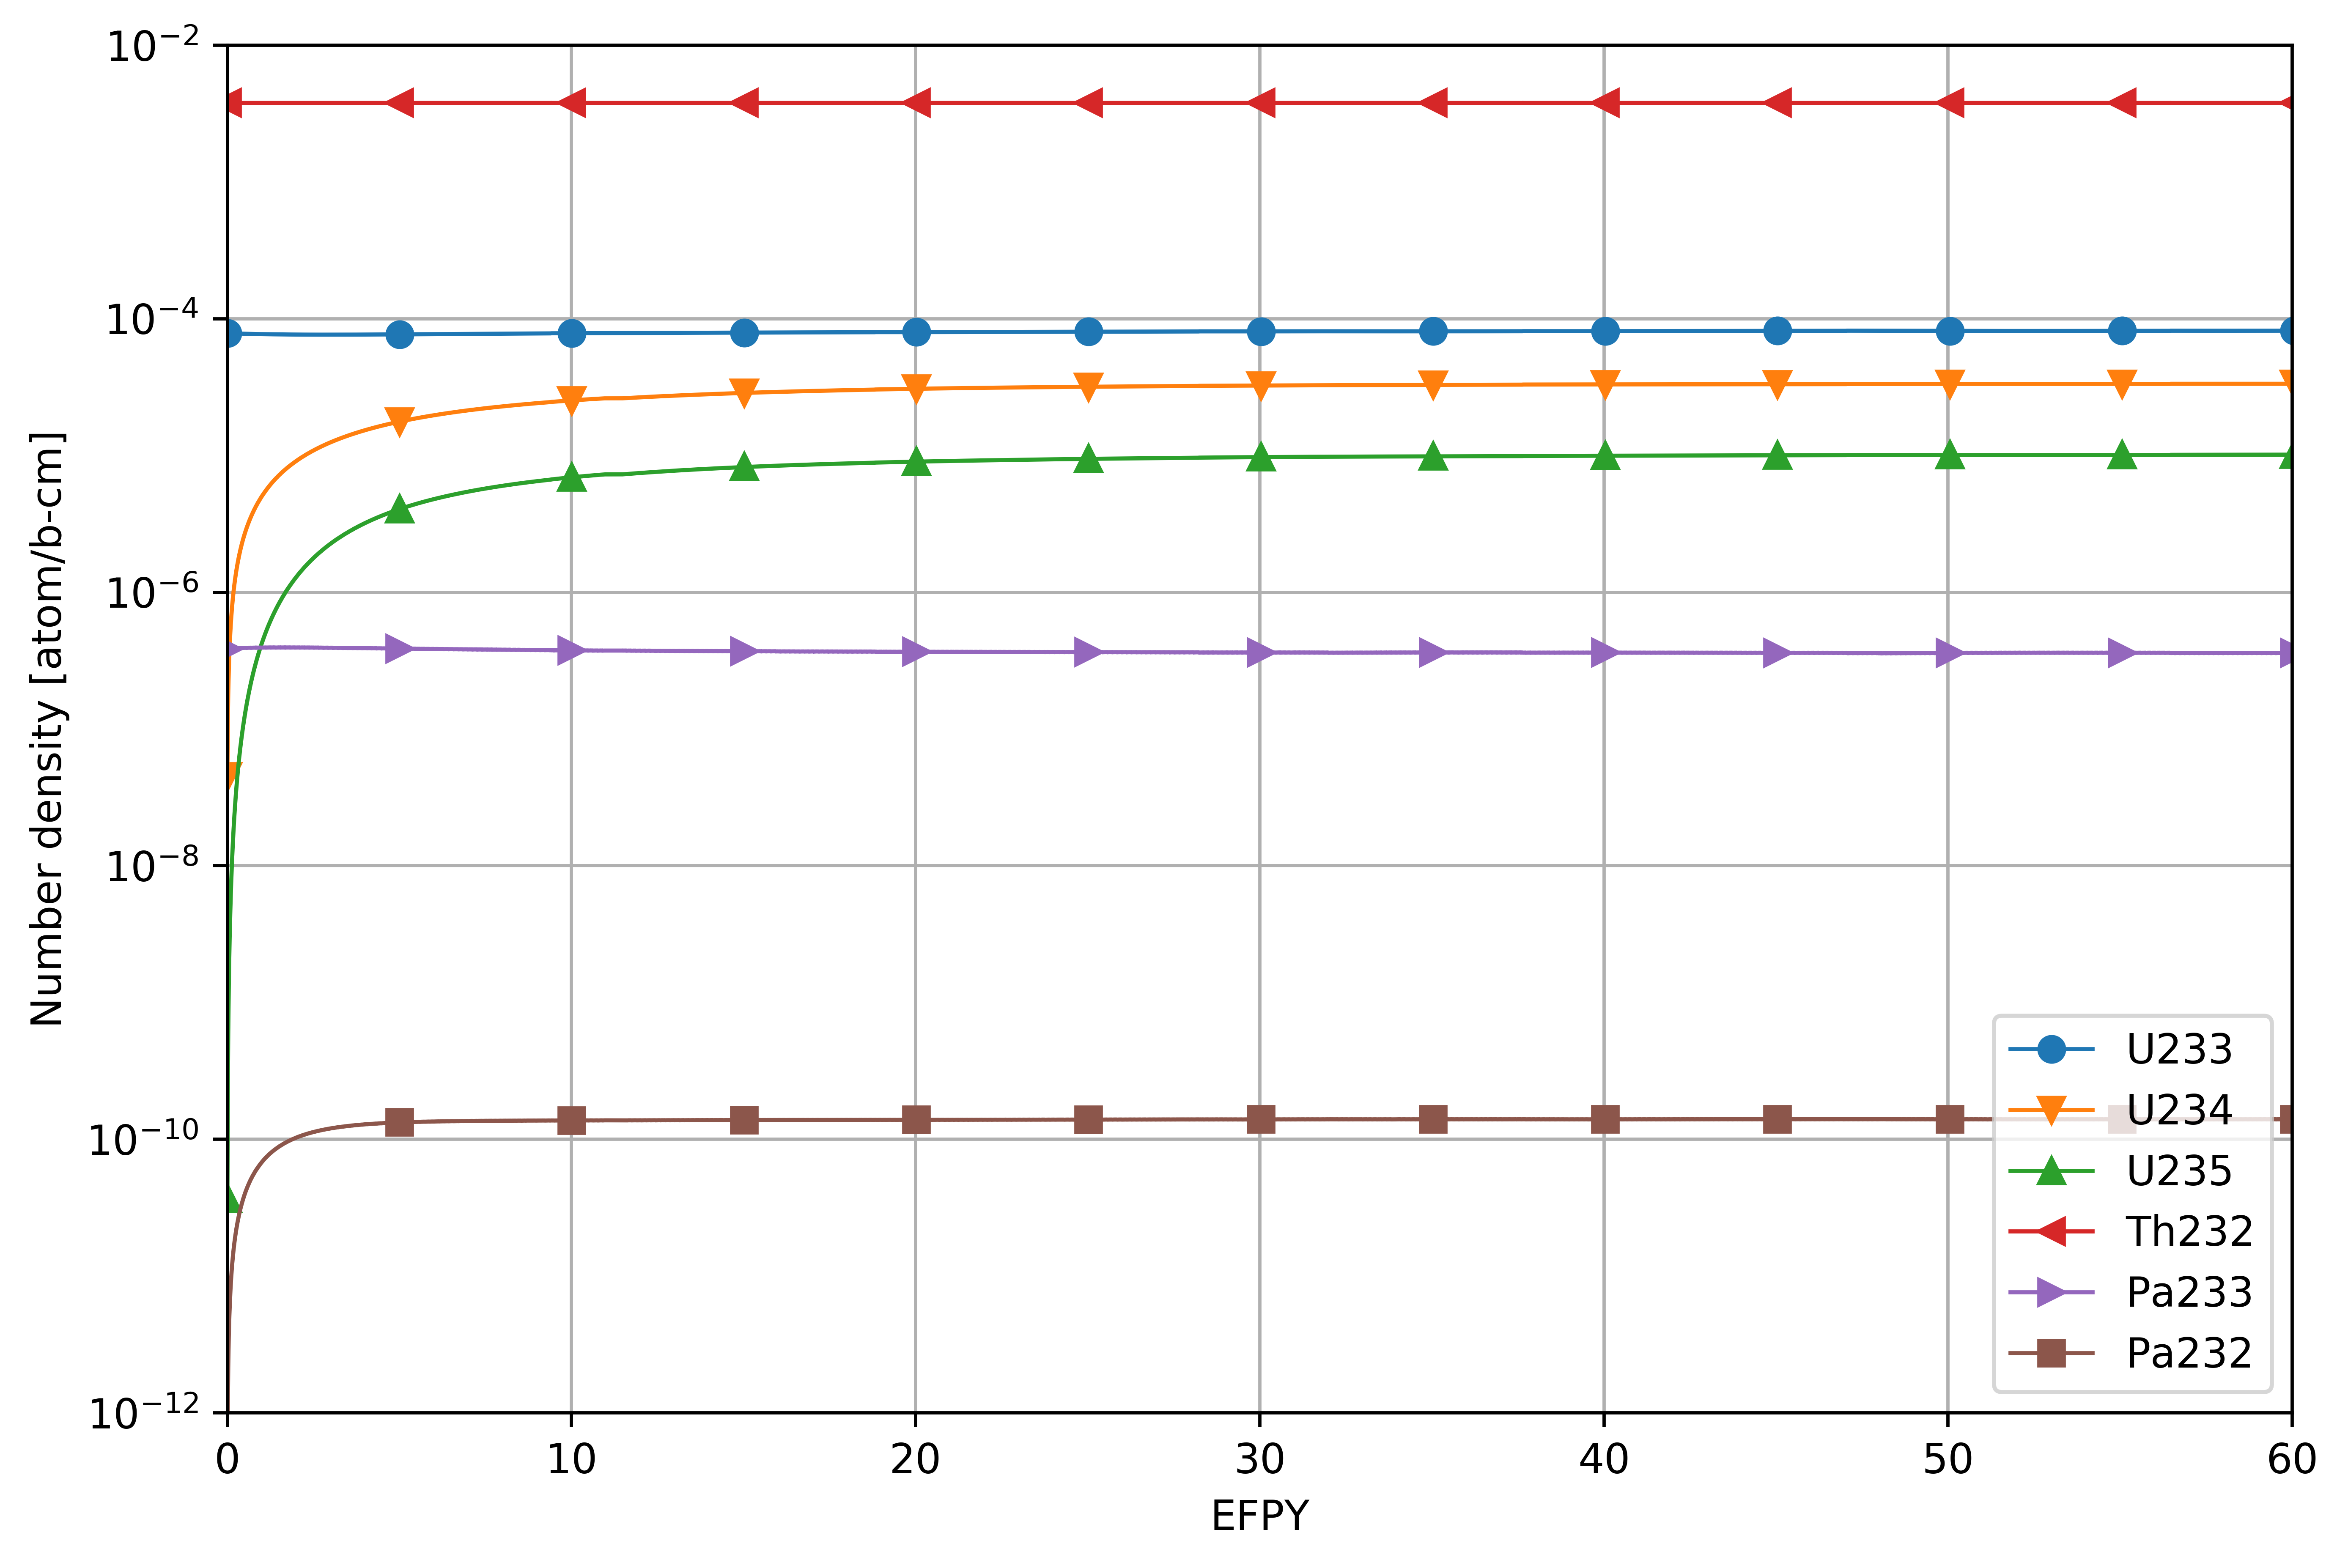
\includegraphics[width=\textwidth]{ch3/major_isotopes_adens.png}
	\caption{The number density of major nuclides during 60 years of reactor 
		operation (reproduced from Rykhlevskii \emph{et al.}  
		\cite{rykhlevskii_modeling_2019}).}
	\label{fig:adens_eq}
\end{figure}
\begin{figure}[t] % replace 't' with 'b' to 
	\centering
	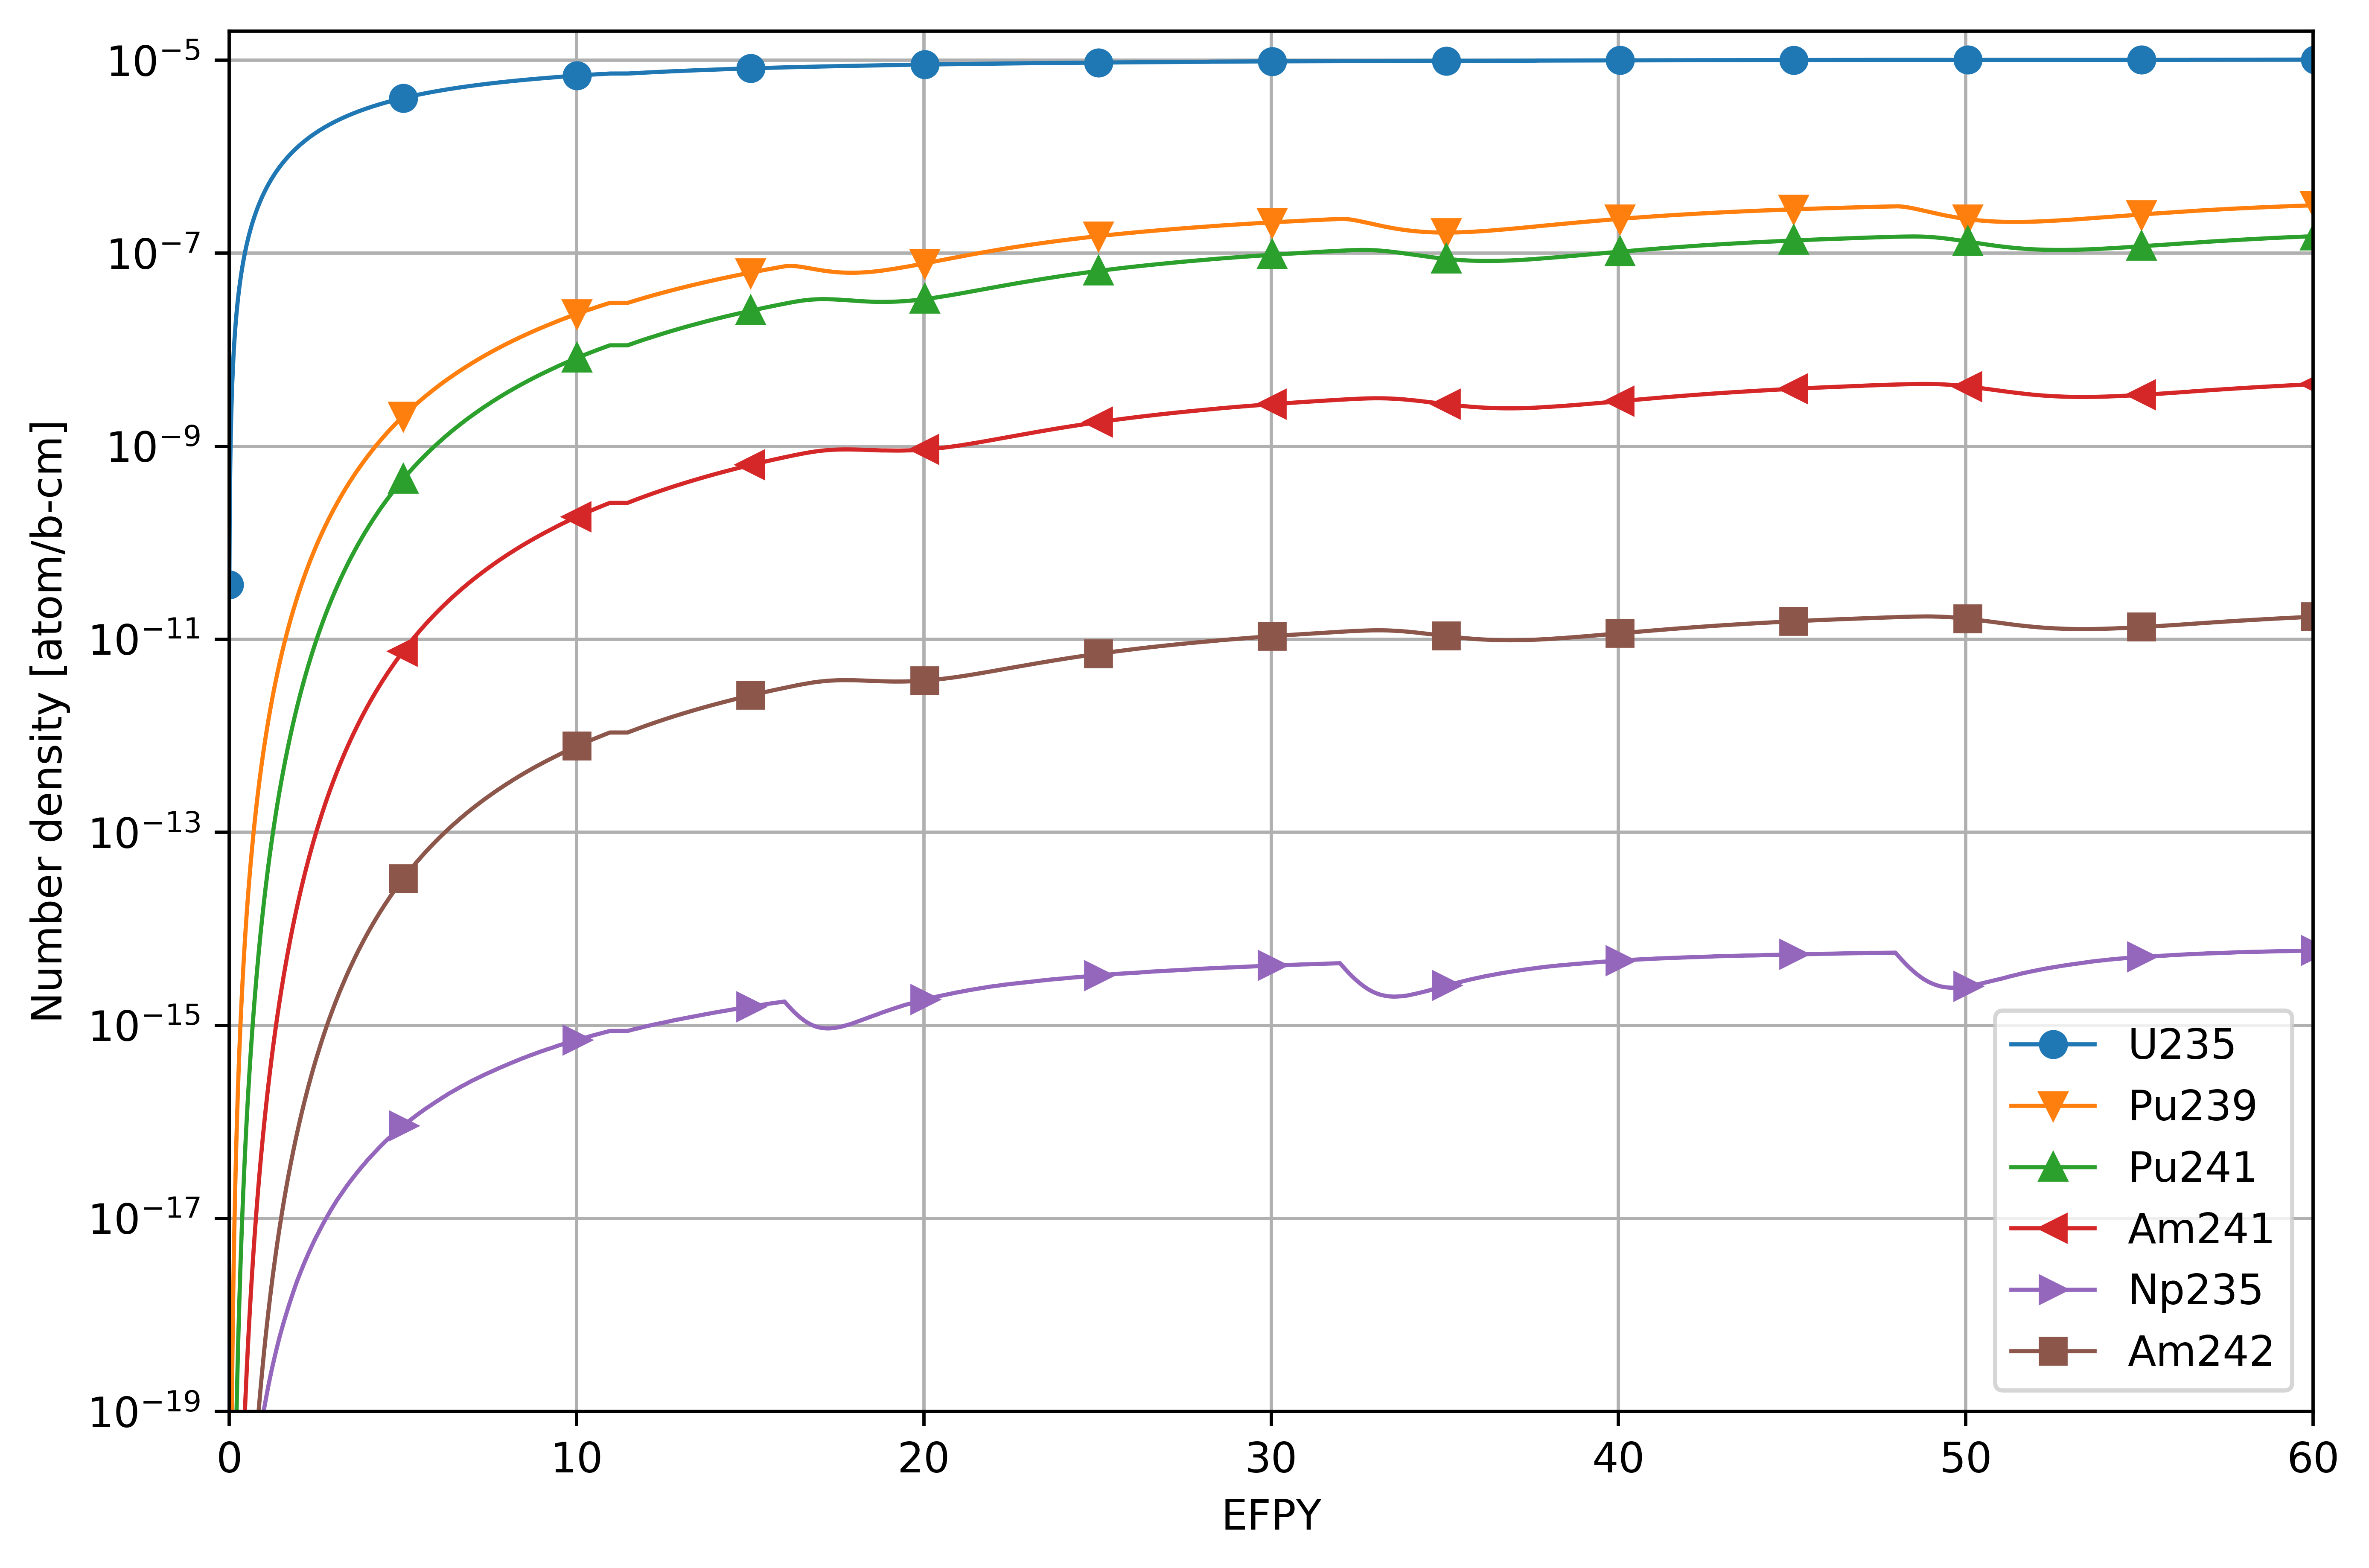
\includegraphics[width=\textwidth]{ch3/fissile_short.png}
	\vspace{-6mm}
	\caption{The number density of \emph{fissile in epithermal spectrum} 
	nuclides during 60 years of the reactor operation (reproduced from 
		Rykhlevskii \emph{et al.} \cite{rykhlevskii_modeling_2019}).}
	\label{fig:fissile_short}
\end{figure}
\FloatBarrier

\subsection{Neutron spectrum}
Figure~\ref{fig:spectrum} shows the normalized neutron flux spectrum for the 
full-core \gls{MSBR} model in the energy range from $10^{-8}$ to $10$ MeV. The 
neutron energy spectrum at equilibrium is harder than at startup due to 
plutonium and other strong absorbers accumulating in the core during reactor 
operation.  

Figure~\ref{fig:spectrum_zones} shows that zone I produced more thermal  
neutrons than zone II, corresponding to a majority of fissions occurring in 
the central part of the core. In the undermoderated zone II, the neutron 
energy spectrum is harder, which leads to more intensive neutron capture by 
$^{232}$Th and helps achieve a relatively high breeding ratio. Moreover, the 
(n,$\gamma$) resonance energy range in $^{232}$Th is from 10$^{-4}$ to 
10$^{-2}$ MeV. Therefore, the moderator-to-fuel ratio for zone II was chosen 
to shift the neutron energy spectrum in this range. Furthermore, in the 
central core region (zone I), the neutron energy spectrum shifts to a harder 
spectrum over 20 years of reactor operation; meanwhile, in the outer core 
region (zone II), a similar spectral shift takes place at a reduced scale. 
These results are in good agreement with the original ORNL report 
\cite{robertson_conceptual_1971} and the most recent whole-core steady-state 
study \cite{park_whole_2015}.
\begin{figure}[htp!] % replace 't' with 'b'         to force it to 
	\centering
	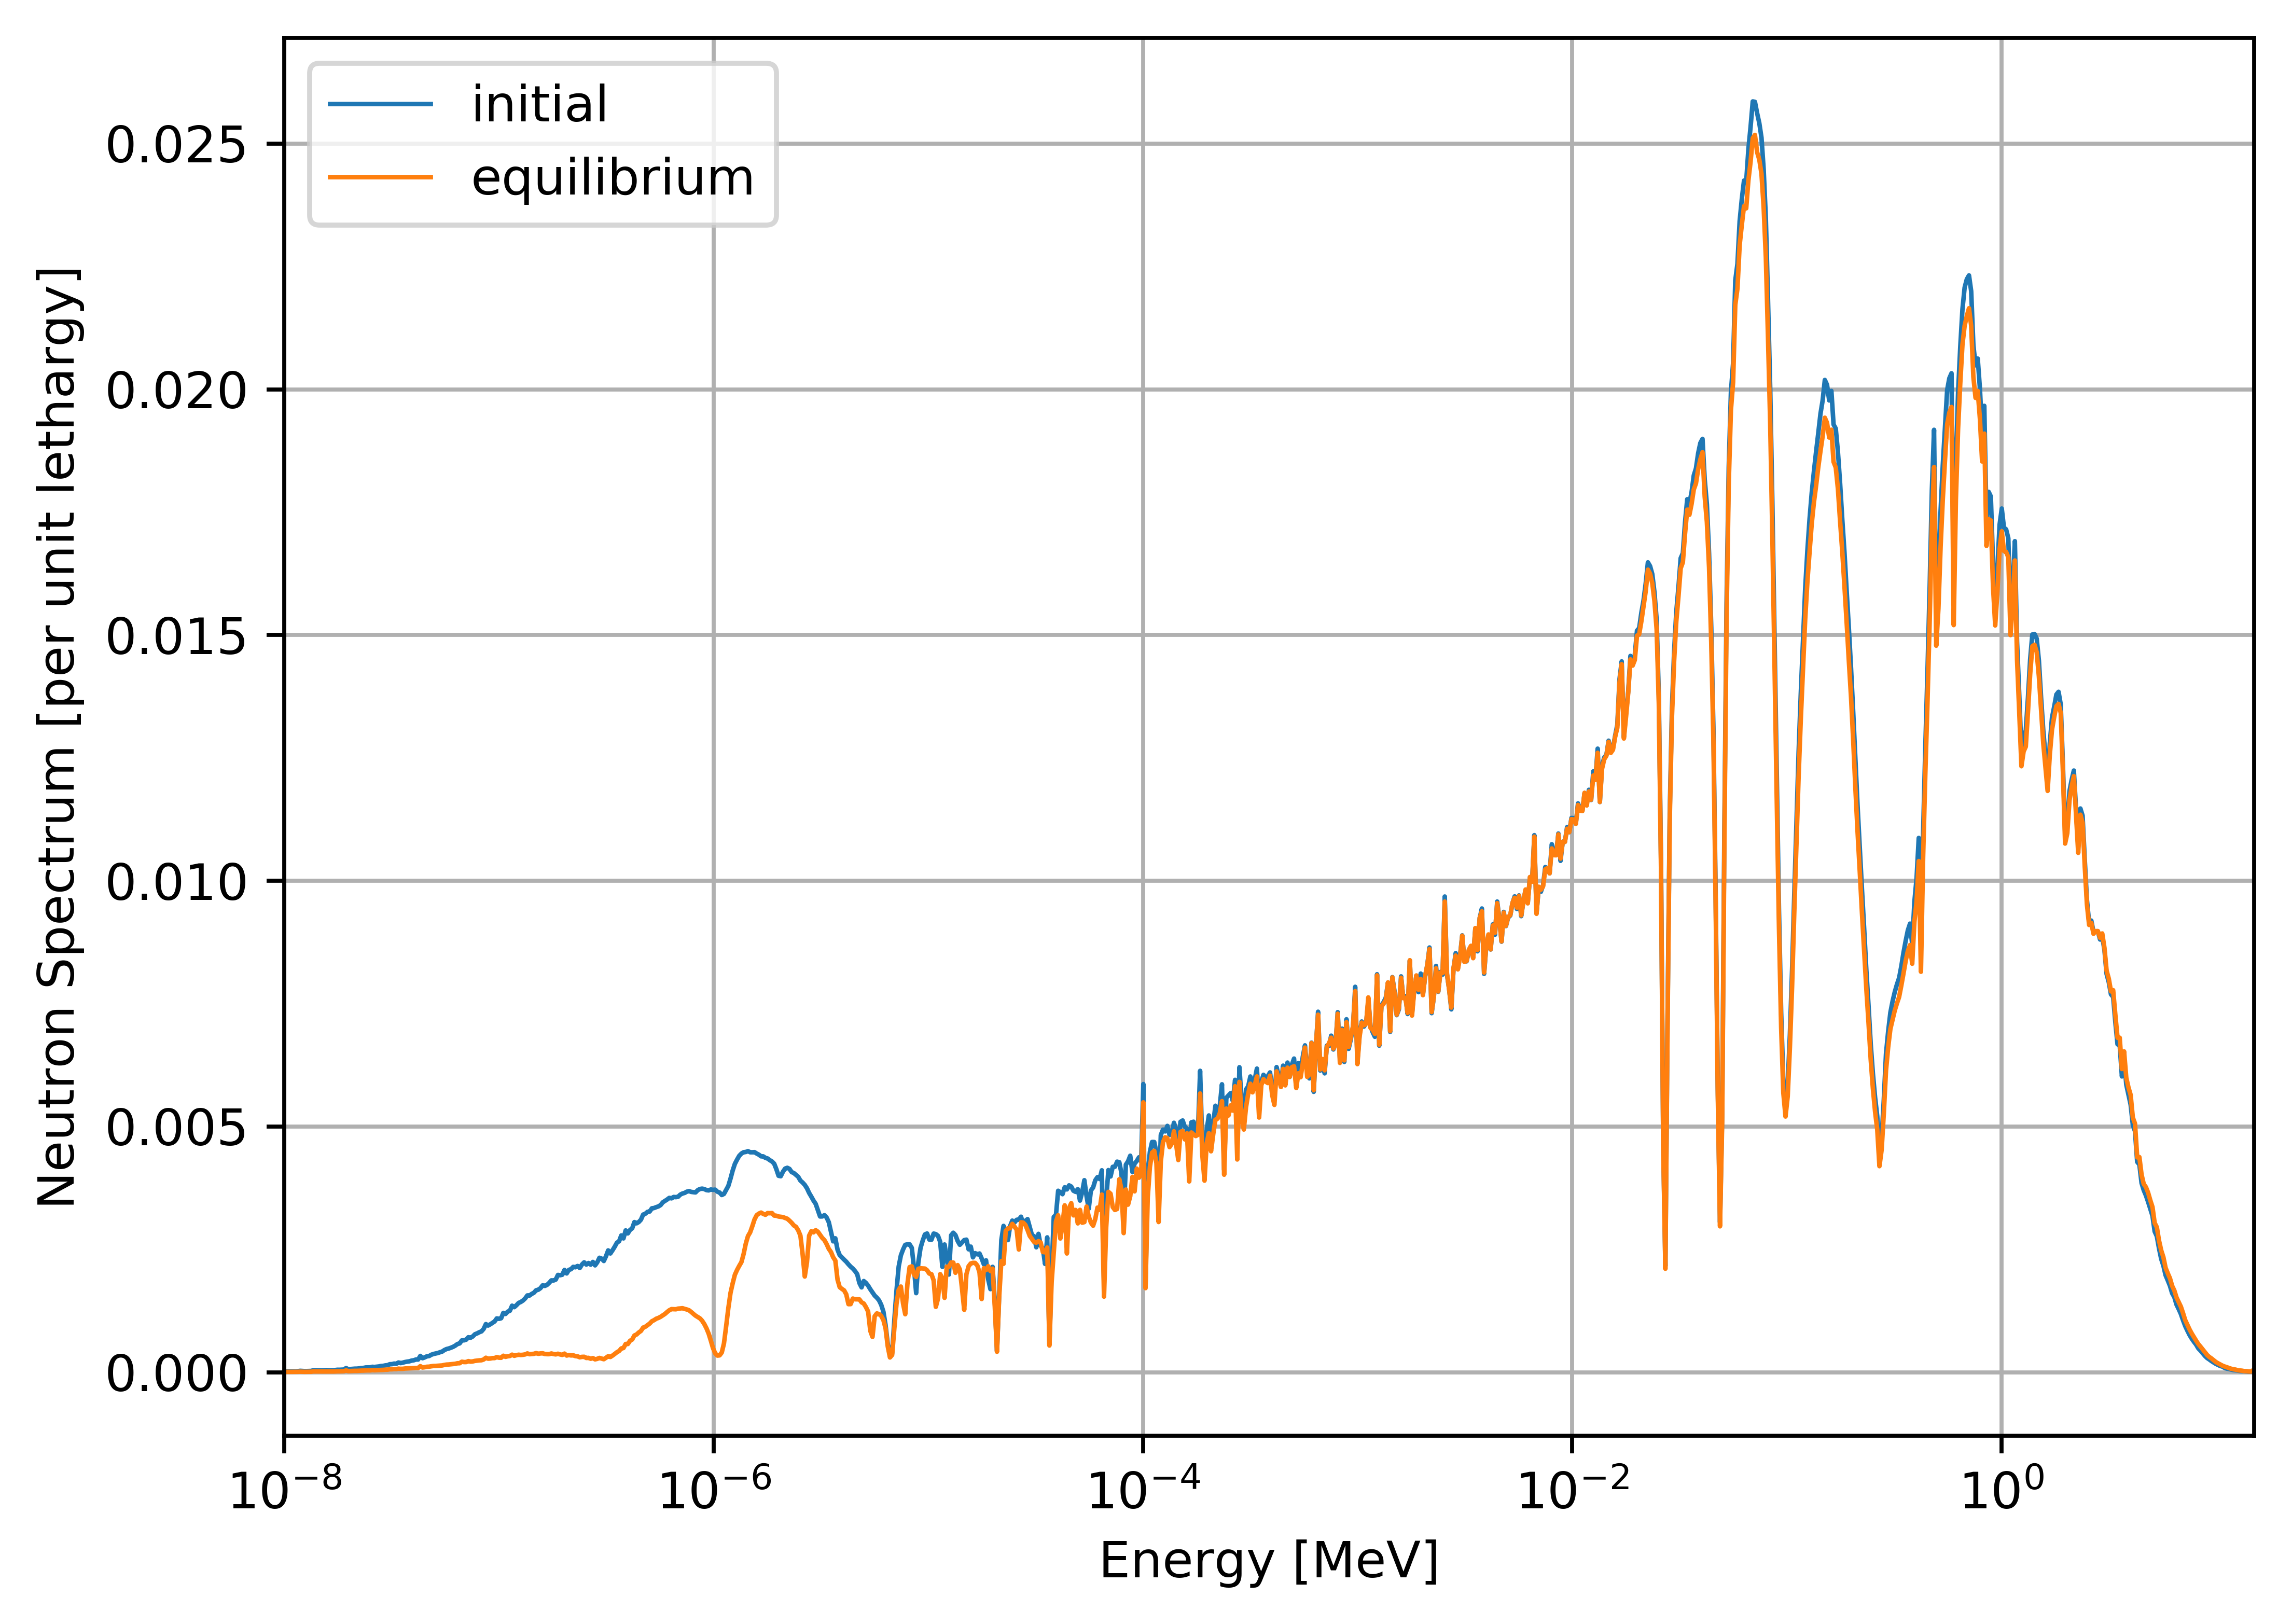
\includegraphics[width=0.85\textwidth]{ch3/spectrum.png}
	\caption{The neutron flux energy spectrum for initial and equilibrium  
	state normalized by unit lethargy (reproduced from Rykhlevskii 
	\emph{et al.} \cite{rykhlevskii_modeling_2019}).}
	\label{fig:spectrum}
\end{figure}
\begin{figure}[htp!] % replace 't' with 'b' to force it to 
	\centering
	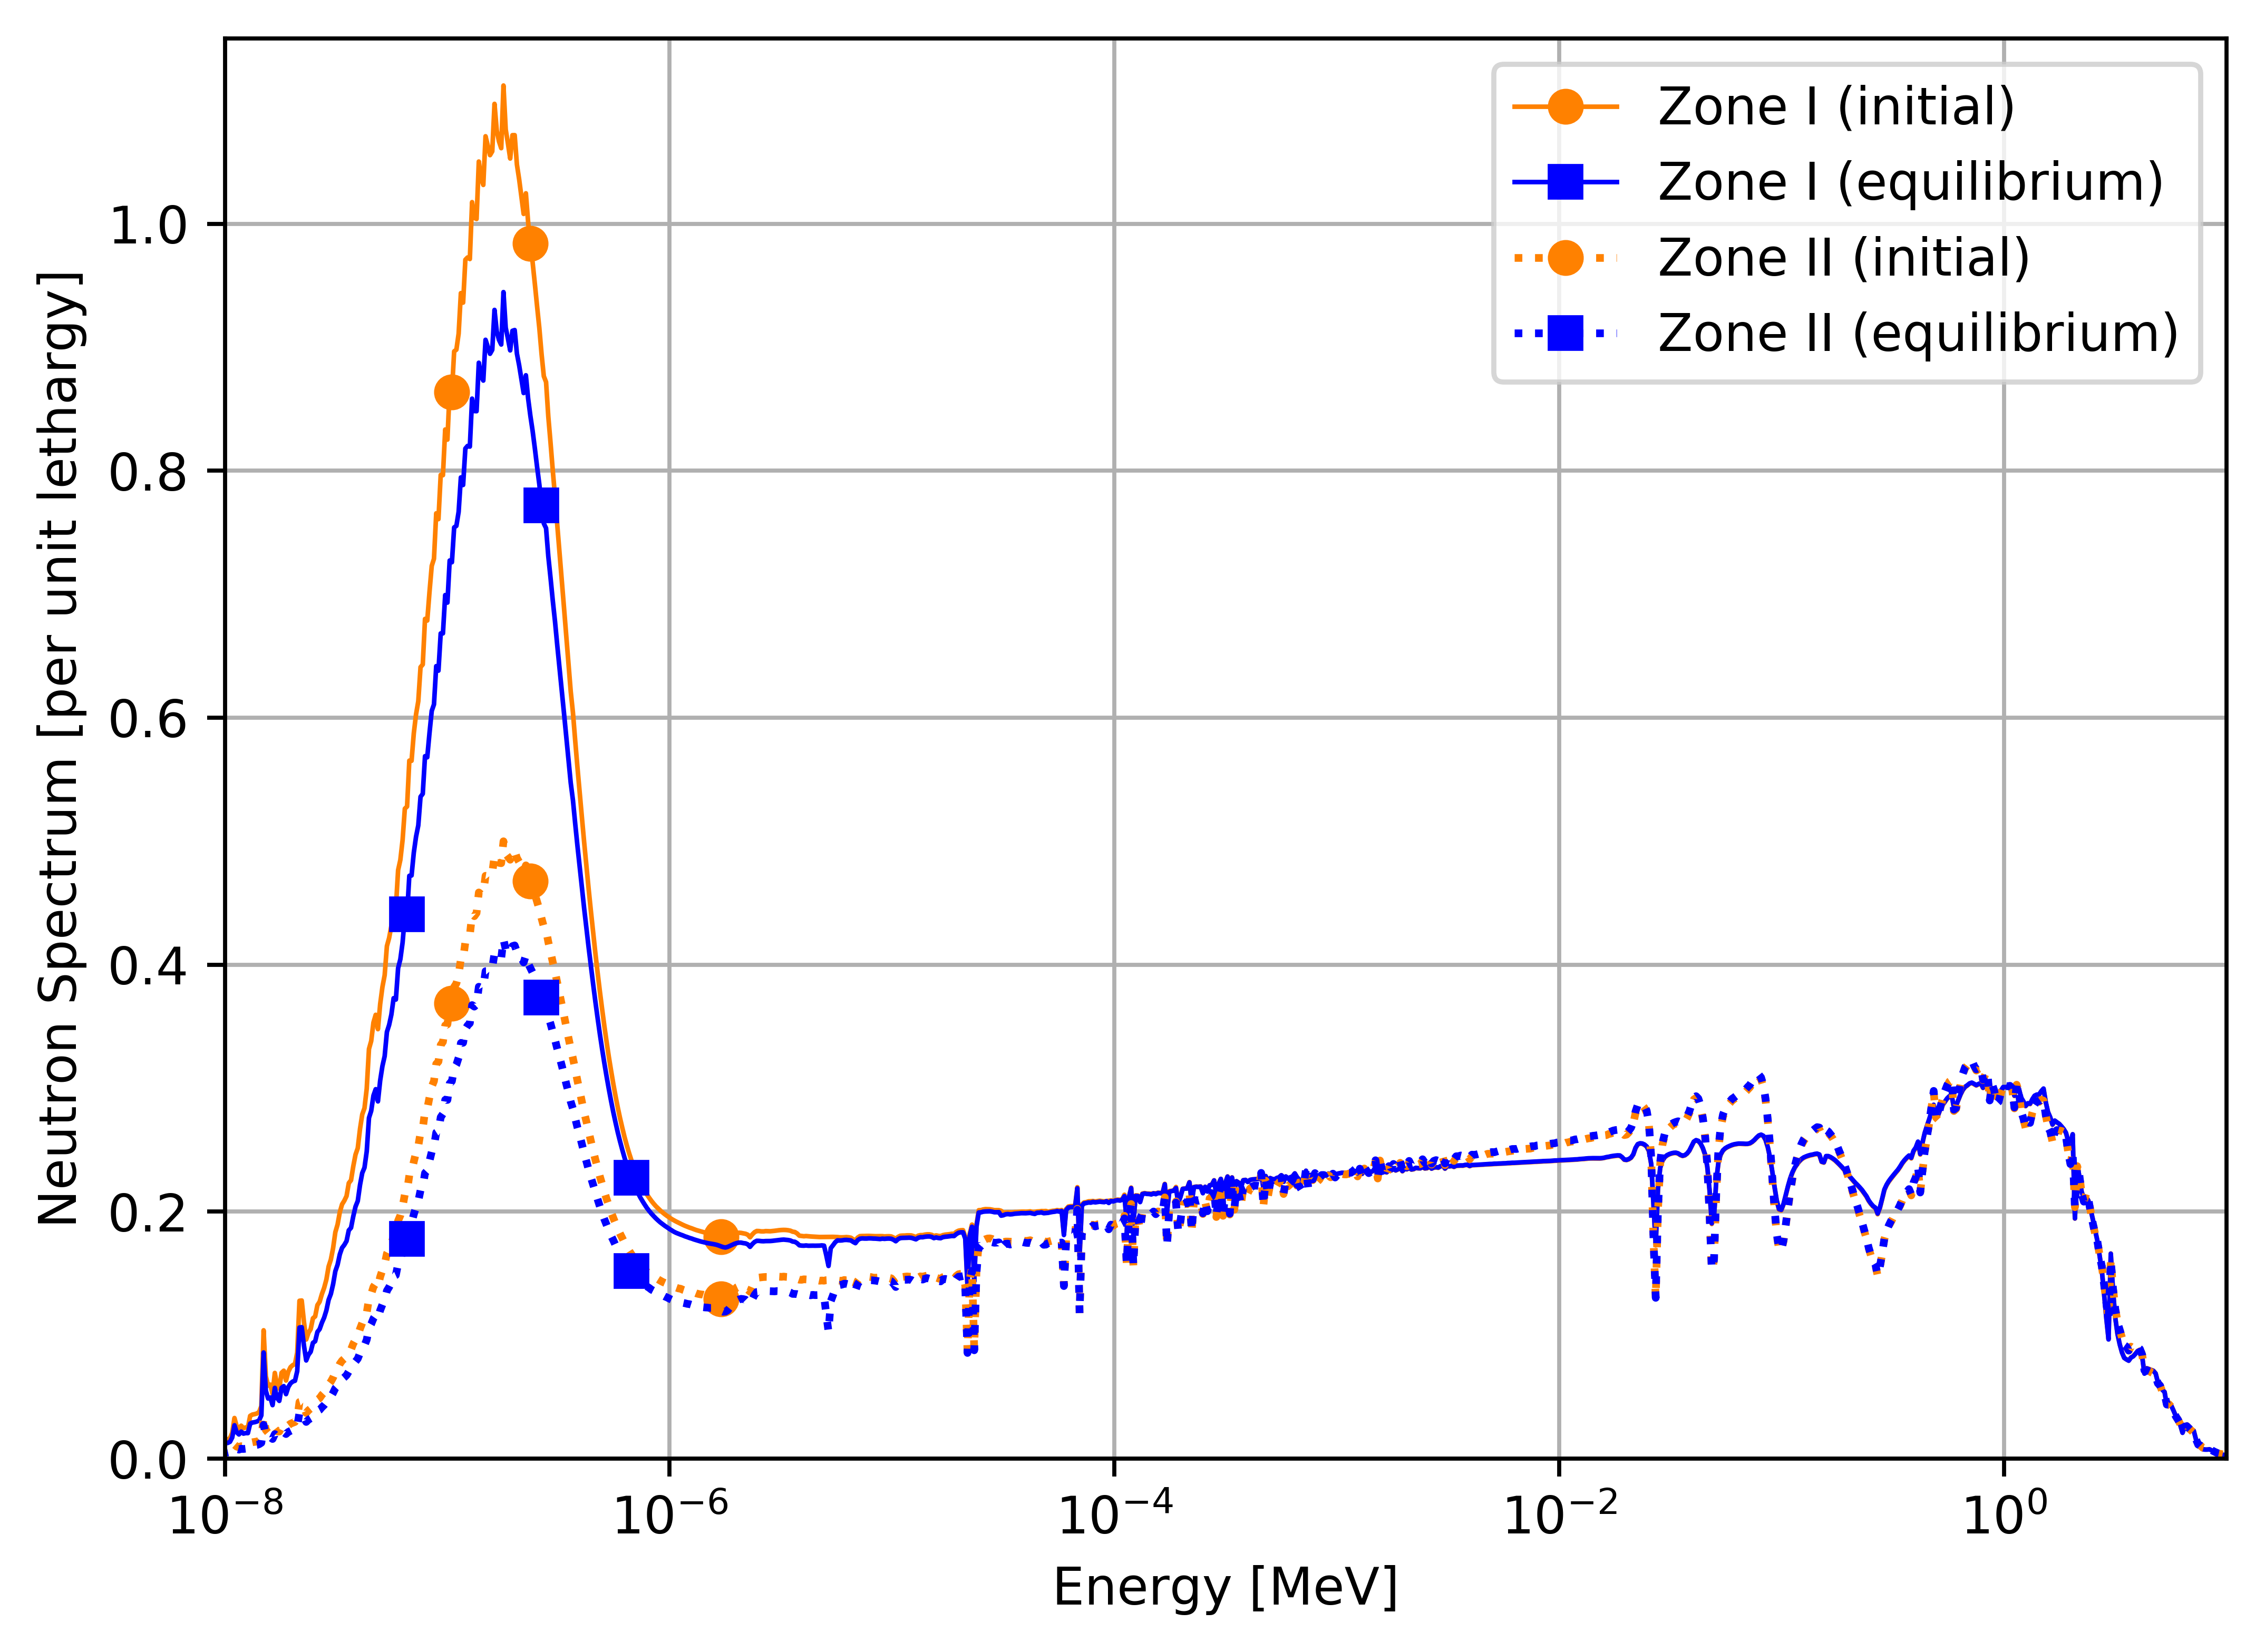
\includegraphics[width=0.85\textwidth]{ch3/spectrum_zones.png} 
	\caption{The neutron flux energy spectrum for initial and equilibrium  
		state normalized by unit lethargy (reproduced from 
		Rykhlevskii \emph{et al.} \cite{rykhlevskii_modeling_2019}).}
	\label{fig:spectrum_zones}
\end{figure}

It is important to obtain the epithermal and thermal spectra to produce 
$^{233}$U from $^{232}$Th because the radiative capture cross section of 
thorium decreases monotonically from $10^{-10}$ MeV to $10^{-5}$ MeV. 
Hardening the spectrum tends to significantly increase resonance absorption in 
thorium and decrease absorptions in fissile and construction materials. 

\subsection{Neutron flux}
Figure~\ref{fig:radial_flux} shows the radial distribution of fast and thermal 
neutron flux for initial and equilibrium compositions. The neutron fluxes have 
similar shapes for both compositions, but the equilibrium case has a harder 
spectrum. A significant spectral shift was observed in the central region of 
the core (zone I), while for the outer region (zone II), it is negligible for 
fast but notable for thermal neutrons. These neutron flux radial distributions 
agree with the fluxes in the original ORNL report 
\cite{robertson_conceptual_1971}. 
Overall, spectrum hardening during \gls{MSBR} operation should be carefully 
studied when designing the reactivity control system.
\begin{figure}[ht!] % replace 't' with 'b' to force it to \centering
	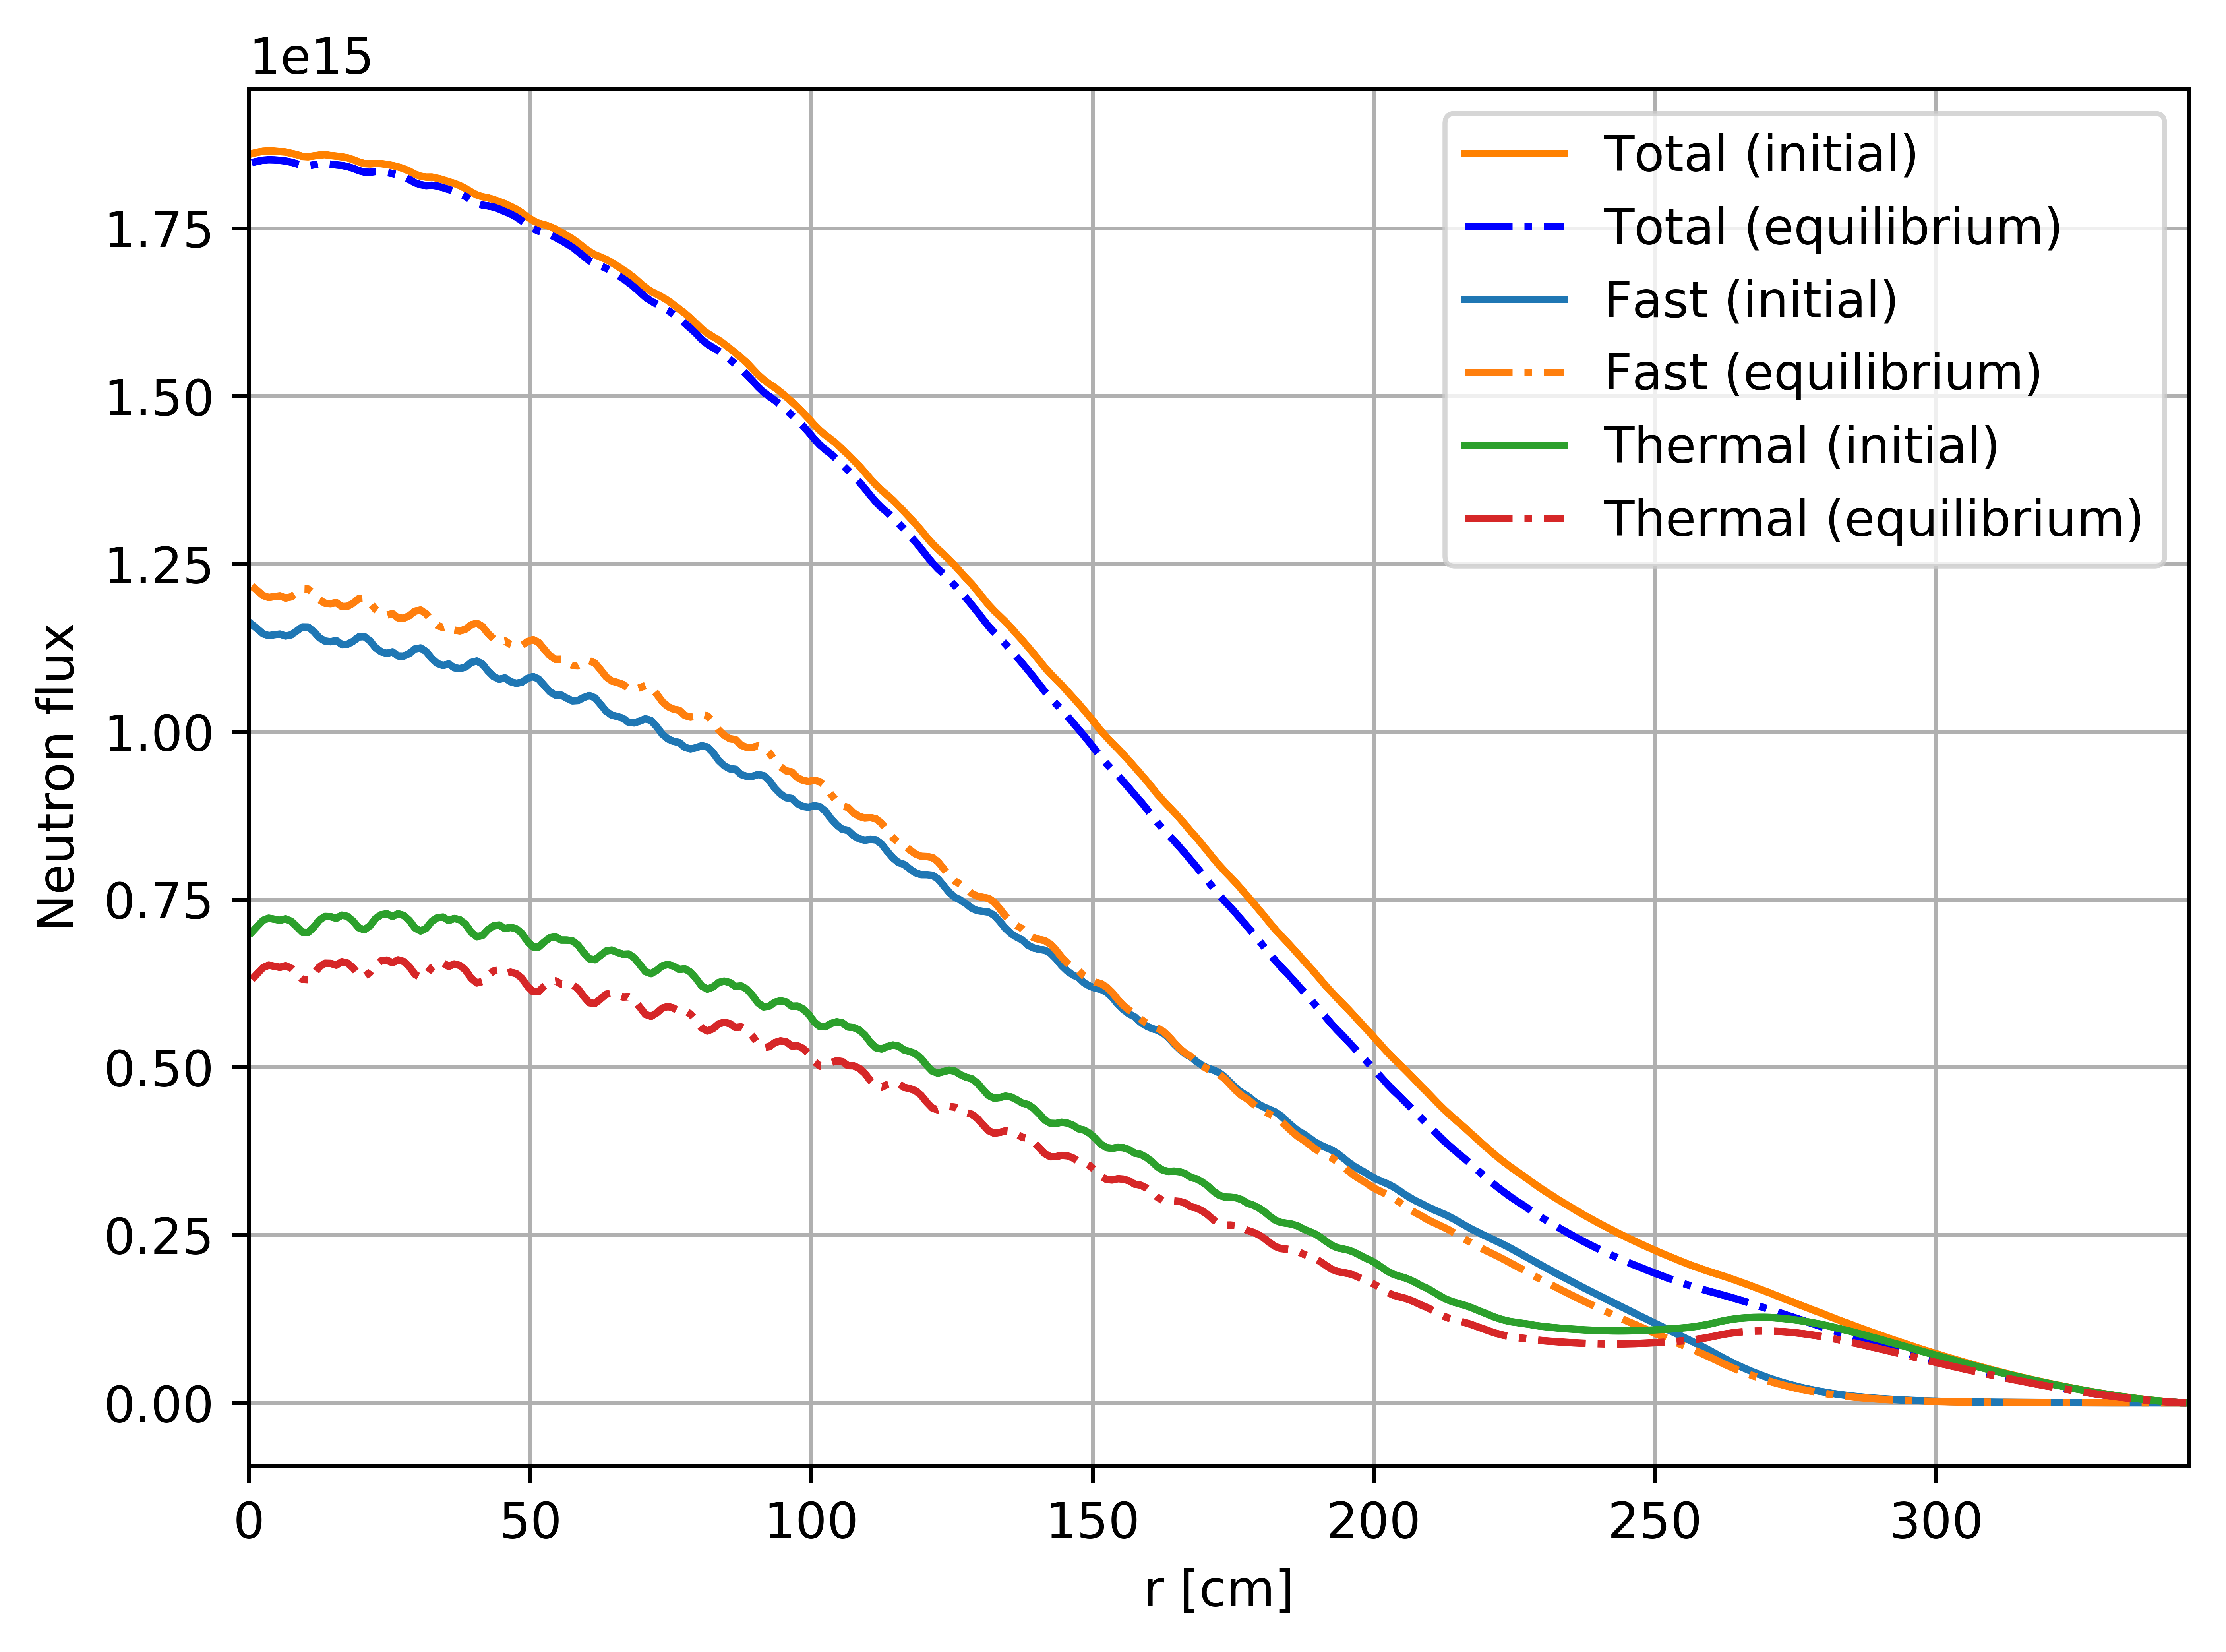
\includegraphics[width=\textwidth]{ch3/radial_flux.png}
	\caption{Radial neutron flux distribution for initial and equilibrium fuel 
	salt compositions (reproduced from Rykhlevskii \emph{et al.} 
	\cite{rykhlevskii_modeling_2019}).}
	\label{fig:radial_flux}
\end{figure}

\subsection{Power and breeding distribution}
Table~\ref{tab:powgen_fraction} shows the power fraction in each zone for 
initial and equilibrium fuel compositions. Figure~\ref{fig:pow_den} reflects 
the normalized power distribution of the \gls{MSBR} quarter core for 
equilibrium fuel salt composition. For both the initial and equilibrium 
compositions, fission primarily occurs in the center of the core, namely zone 
I. The spectral shift during reactor operation results in slightly different 
power fractions at startup and equilibrium, but most of the power is still 
generated in zone I at equilibrium (Table~\ref{tab:powgen_fraction}). 
%%%%%%%%%%%%%%%%%%%%%%%%%%%%%%%%%%%%%%%%
\begin{table}[ht!]
	\caption{Power generation fraction in each zone for initial and 
	equilibrium state (reproduced from Rykhlevskii \emph{et al.} 
	\cite{rykhlevskii_modeling_2019}).}
		\centering
	\begin{tabularx}{0.8\textwidth}{L R R} \hline
		Core region & Initial            & Equilibrium   \\   \hline
		Zone I      & 97.91\%            & 98.12\%   \\
		Zone II     & 2.09\%             & 1.88\%   \\ \hline
	\end{tabularx}
	\label{tab:powgen_fraction}
\end{table}
%%%%%%%%%%%%%%%%%%%%%%%%%%%%%%%%%%%%%%%%%%%%%%%%%%%%%%%%%%%%%%%%%%%%%%%%%%%%%%%
\begin{figure}[ht!] % replace 't' with 'b' to force it to 
	\centering
	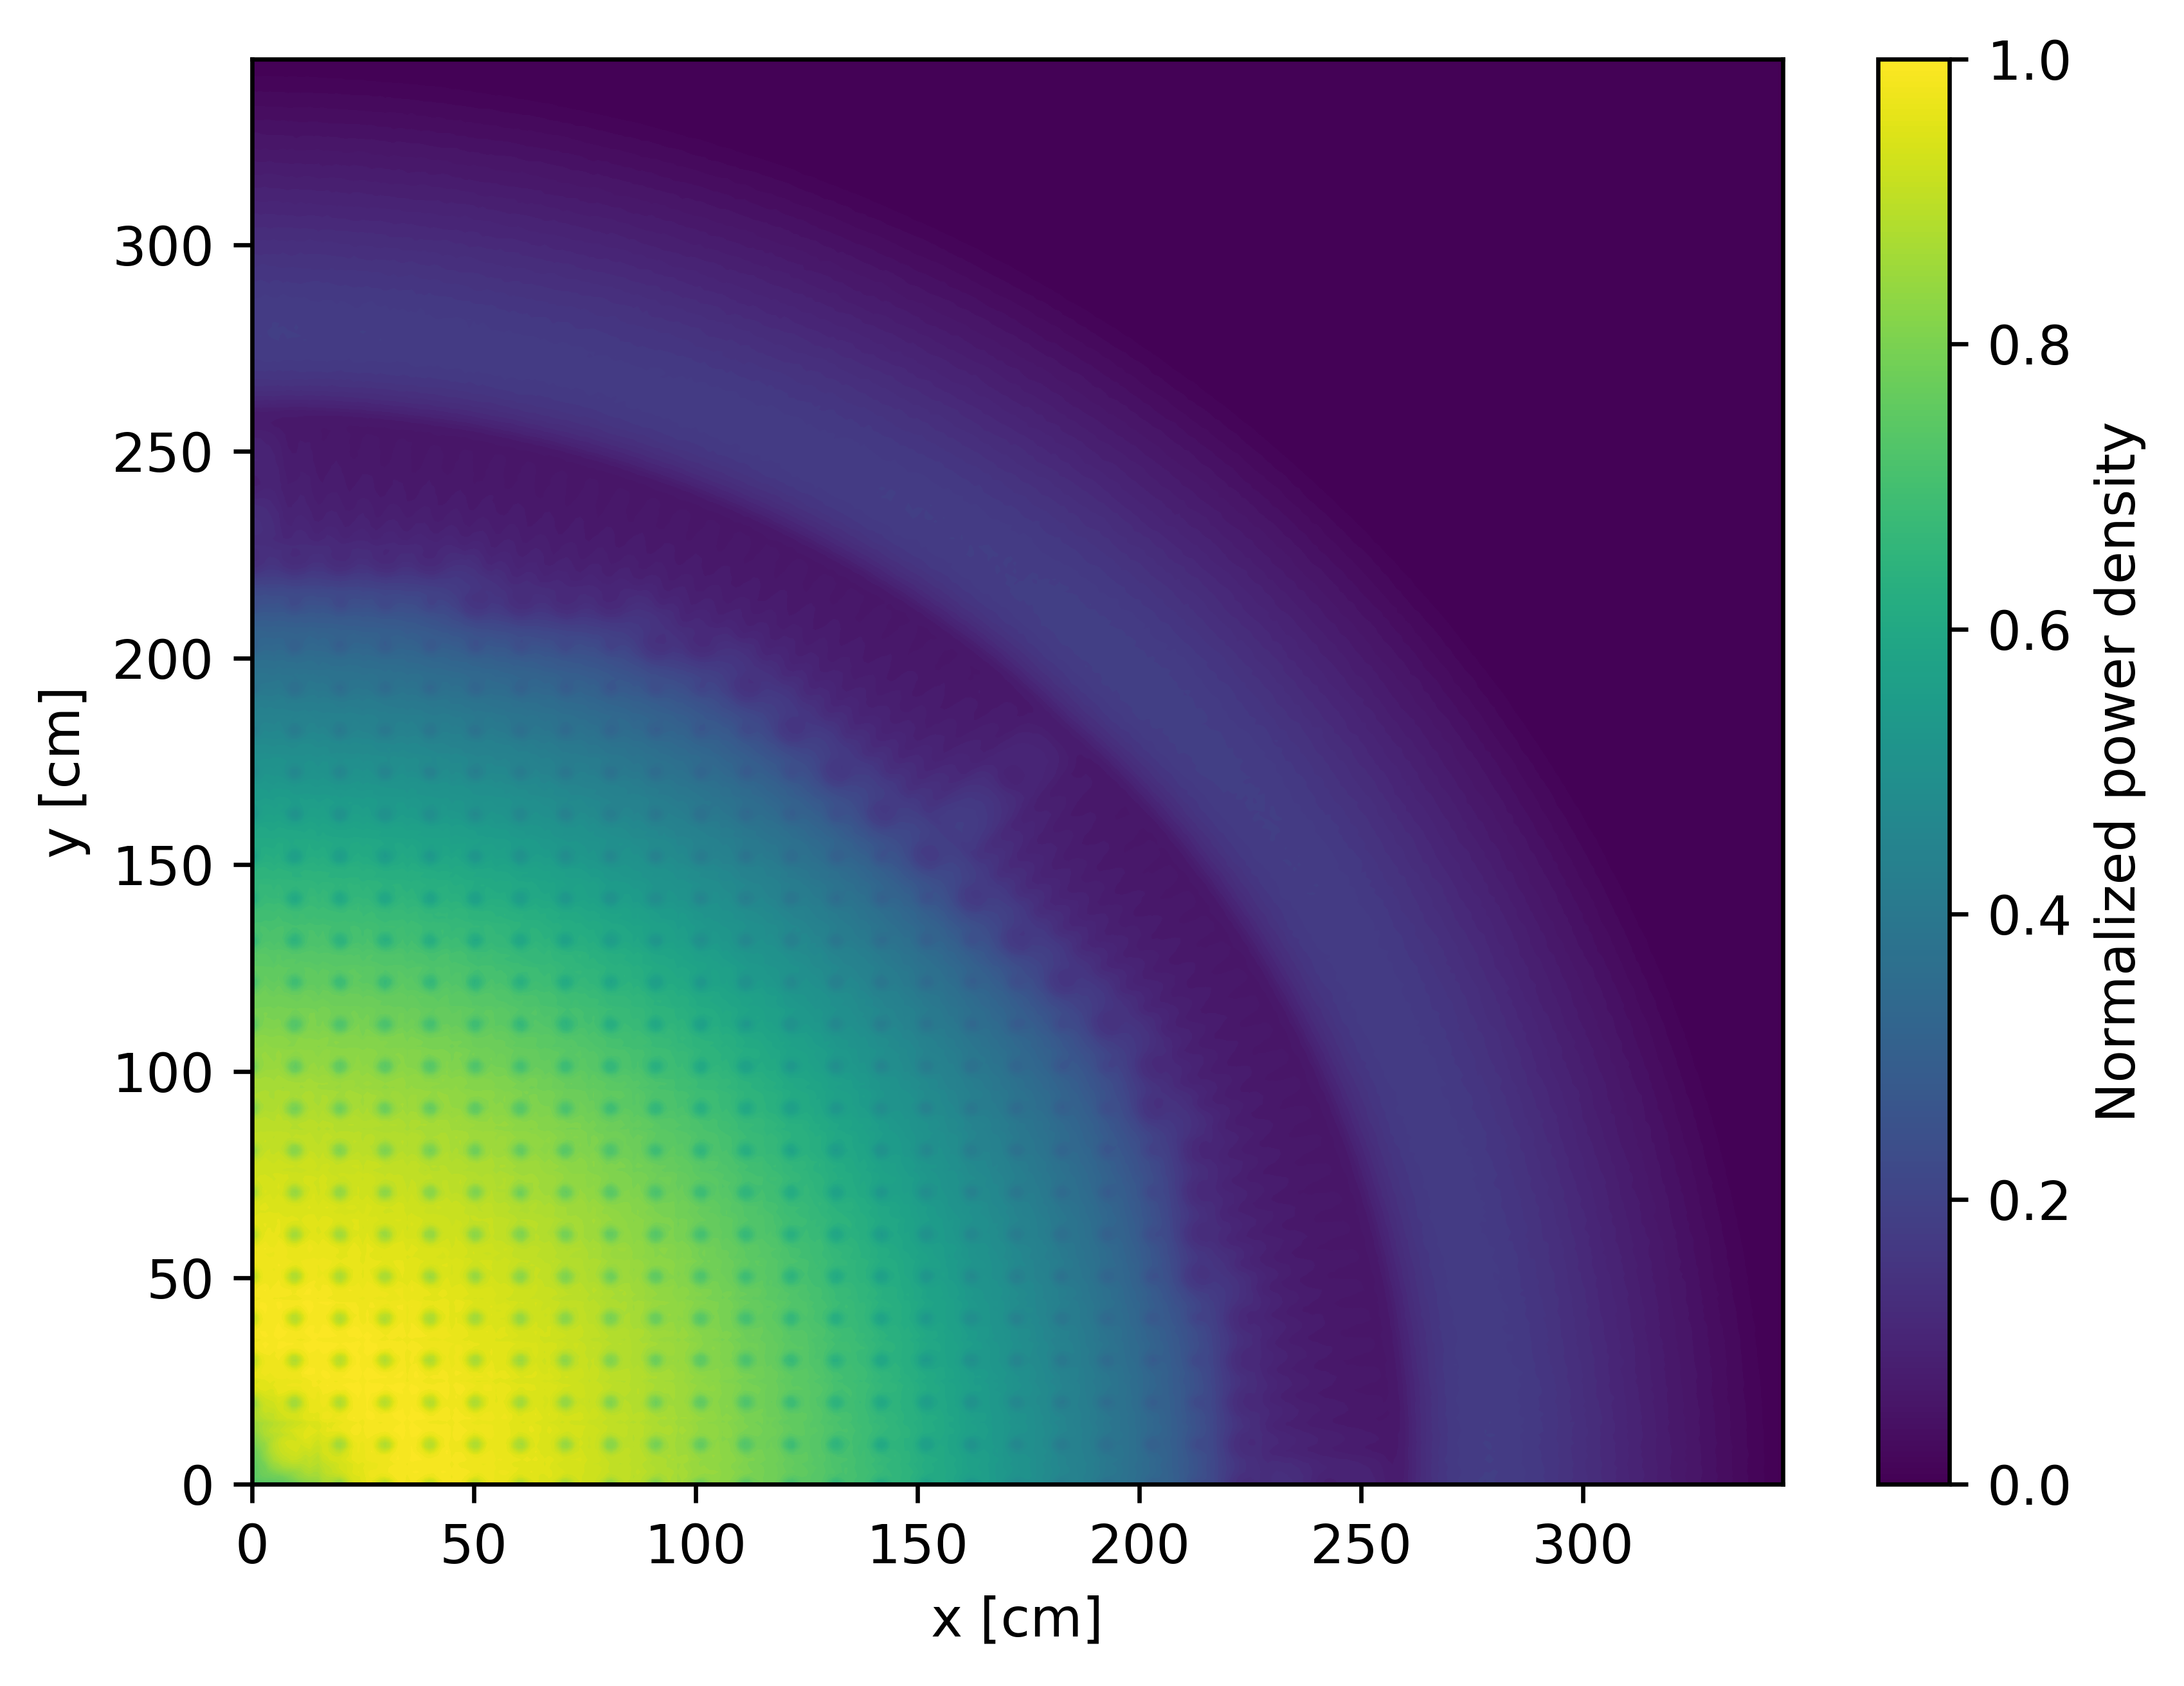
\includegraphics[width=0.82\textwidth]{ch3/power_distribution_eq.png} 
	\vspace{-5mm}
	\caption{Normalized power density for equilibrium fuel salt composition 
		(reproduced from Rykhlevskii \emph{et al.} 
		\cite{rykhlevskii_modeling_2019}).}
	\label{fig:pow_den}
\end{figure}

Figure~\ref{fig:breeding_den} shows the distribution of the neutron capture 
reaction rate for $^{232}$Th normalized by the total neutron flux for the 
initial and equilibrium states. The distribution reflects the spatial 
distribution of $^{233}$U production in the core. $^{232}$Th neutron capture 
produces $^{233}$Th, which then $\beta$-decays to $^{233}$Pa, the precursor 
for $^{233}$U production. Accordingly, this characteristic represents the 
breeding distribution in the \gls{MSBR} core. The power and breeding 
distribution remained almost constant during the reactor operation. Even after 
20 years of operation, most of the power is still generated in zone I.
\begin{figure}[ht!] % replace 't' with 'b' to force it to 
	\centering
	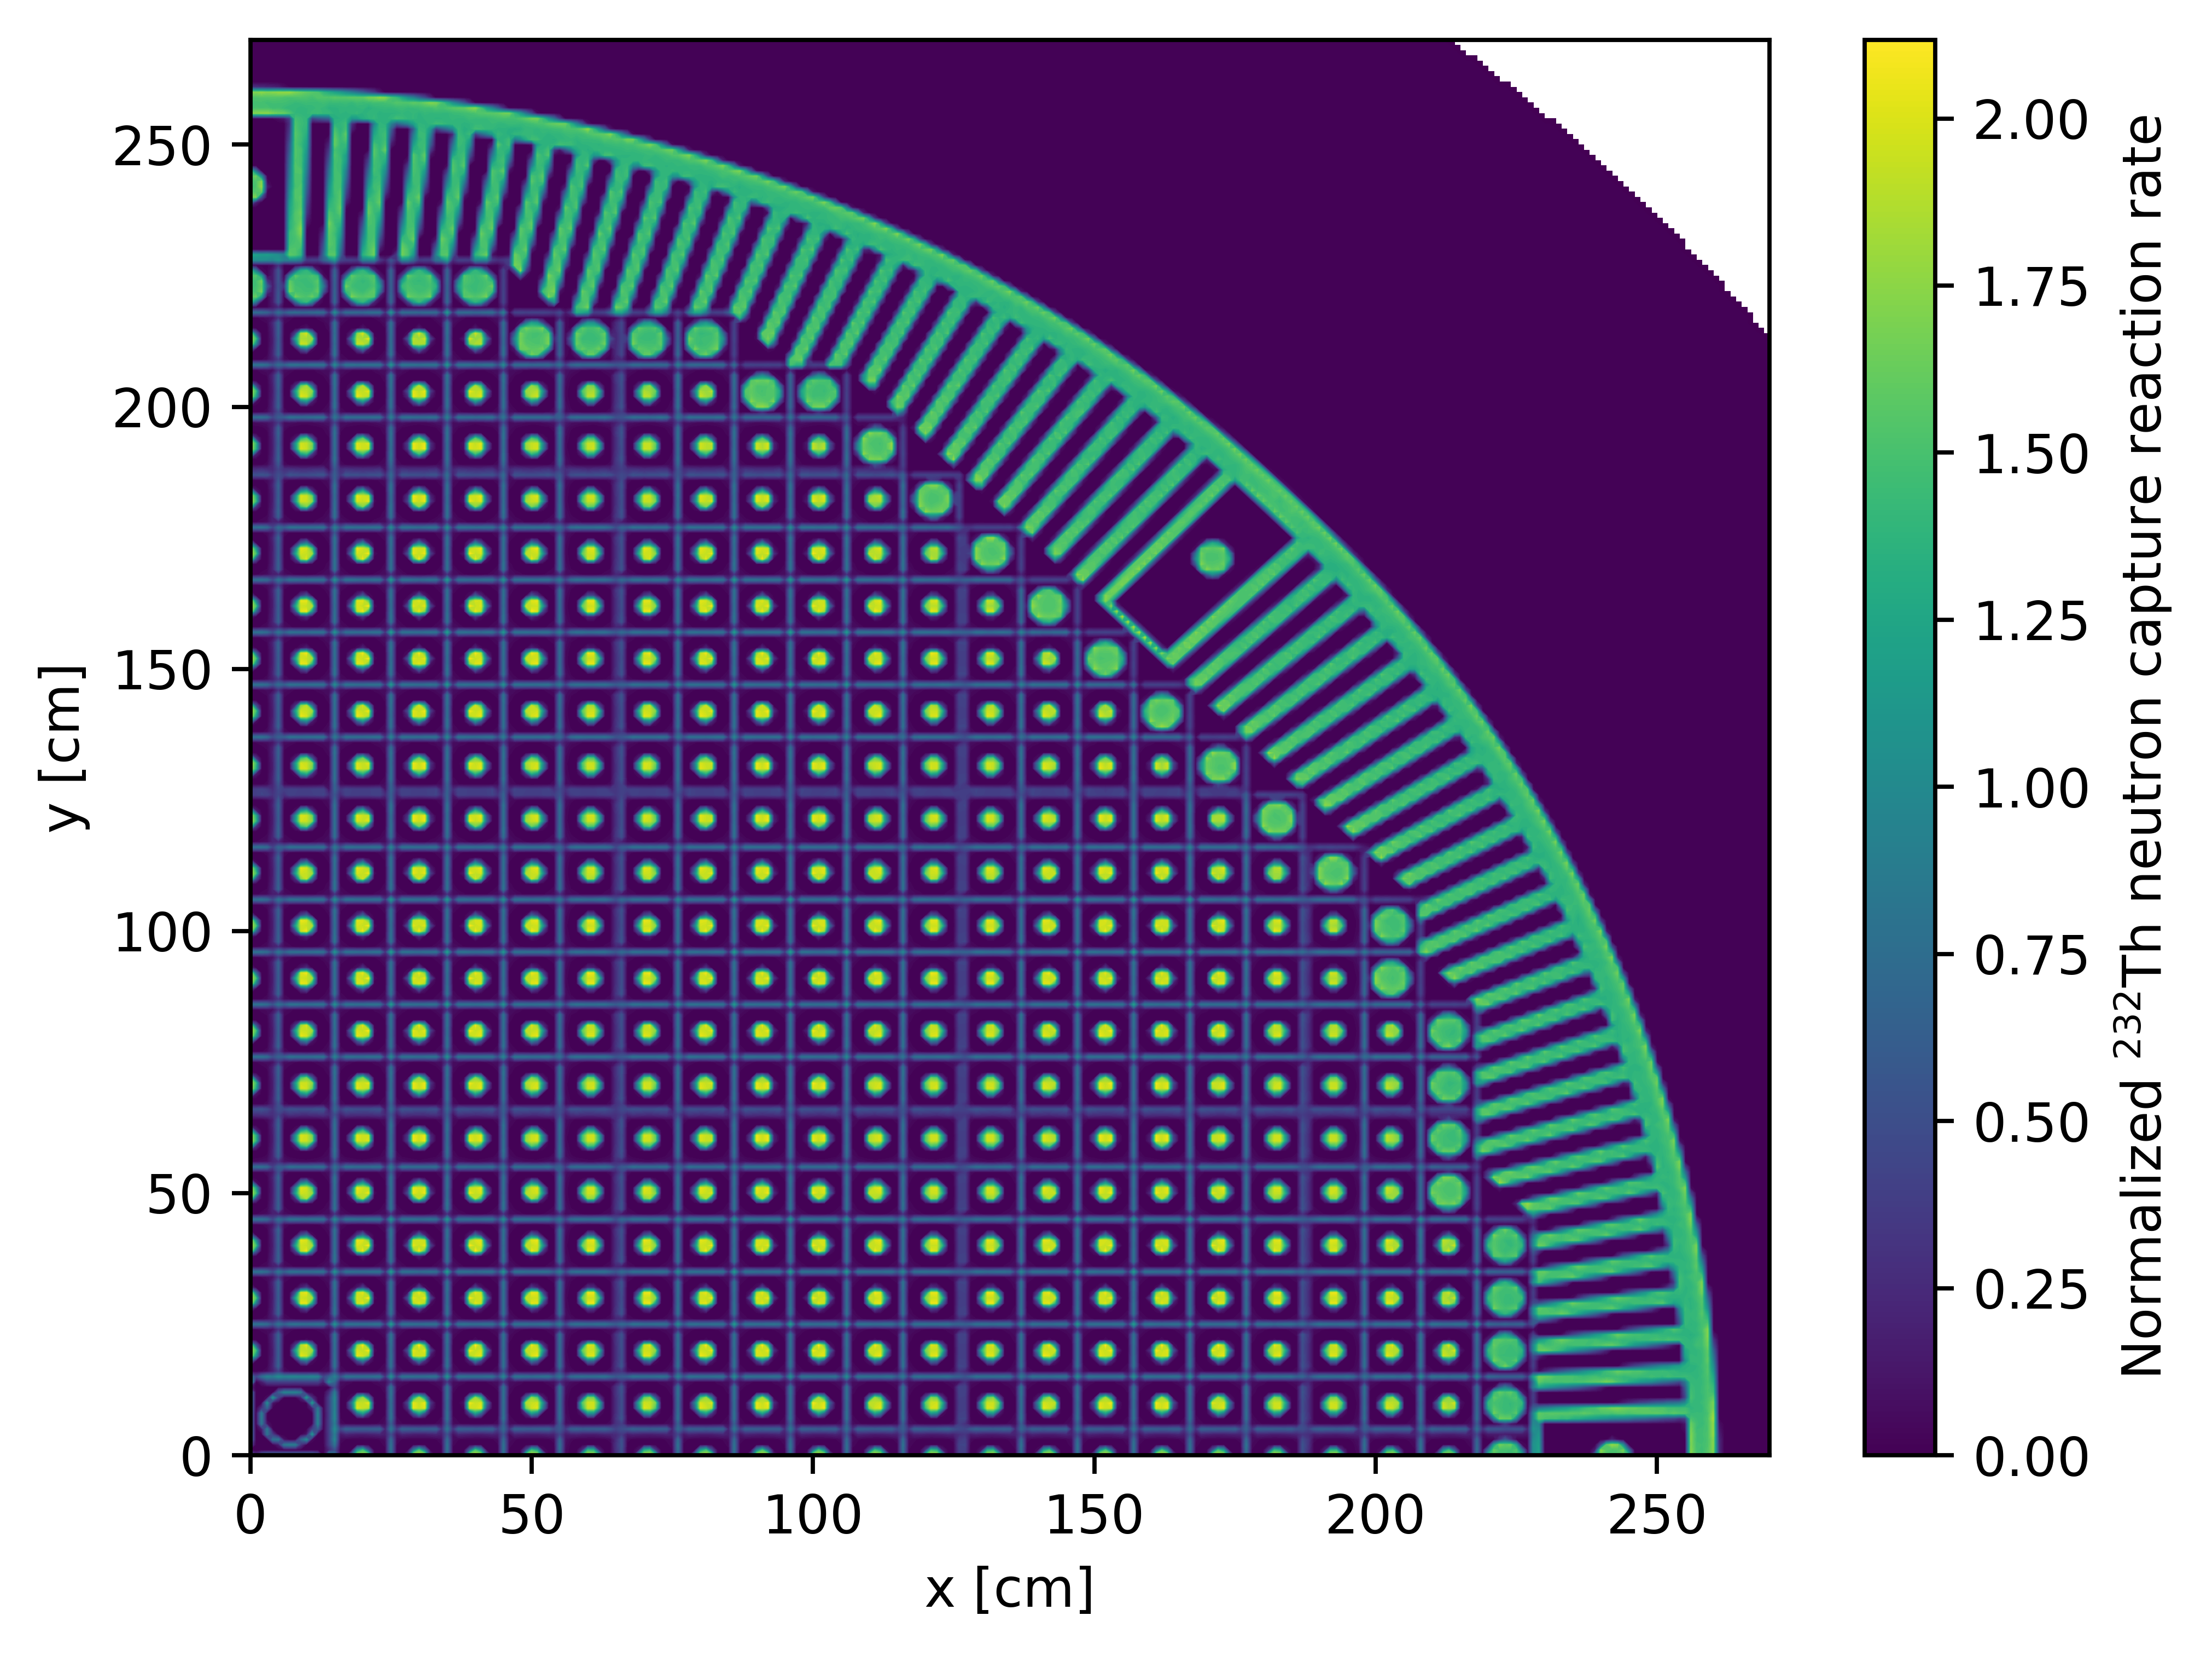
\includegraphics[width=0.82\textwidth]{ch3/breeding_distribution_eq.png} 
		\vspace{-5mm}
	\caption{$^{232}$Th neutron capture reaction rate normalized by total flux 
		for equilibrium fuel salt composition (reproduced from 
		Rykhlevskii \emph{et al.} \cite{rykhlevskii_modeling_2019}).}
	\label{fig:breeding_den}
\end{figure}
\FloatBarrier

%%%%%%%%%%%%%%%%%%%%%%%%%%%%%%%%%%%%%%%%%%%%%%%%%%%%%%%%%%%%%%%%%%%%%%%%%%%%%%%%
\subsection{Thorium refill rate}
In the \gls{MSBR}, the only external feed material flow  is $^{232}$Th. 
Figure~\ref{fig:th_refill} shows the $^{232}$Th feed rate calculated over 60 
years of reactor operation. The $^{232}$Th feed rate fluctuates significantly 
as a result of the batch-wise nature of this online reprocessing approach. 
Figure~\ref{fig:th_refill_zoomed} shows a zoomed thorium feed rate for a short 
150-EFPD interval. Note that the large spikes of up to 36 kg/day in a thorium 
consumption occur every 3435 days. Those spikes happened due to strong 
absorbers' (Rb, Sr, Cs, Ba) removal at the end of the effective cycle (100\% 
of these elements removing every 3435 days of operation). The corresponding 
effective multiplication factor increase (Figure~\ref{fig:keff}) and breeding  
intensification leads to additional $^{232}$Th consumption.  
\begin{figure}[ht!] % replace 't' with 'b' to force it to \centering
	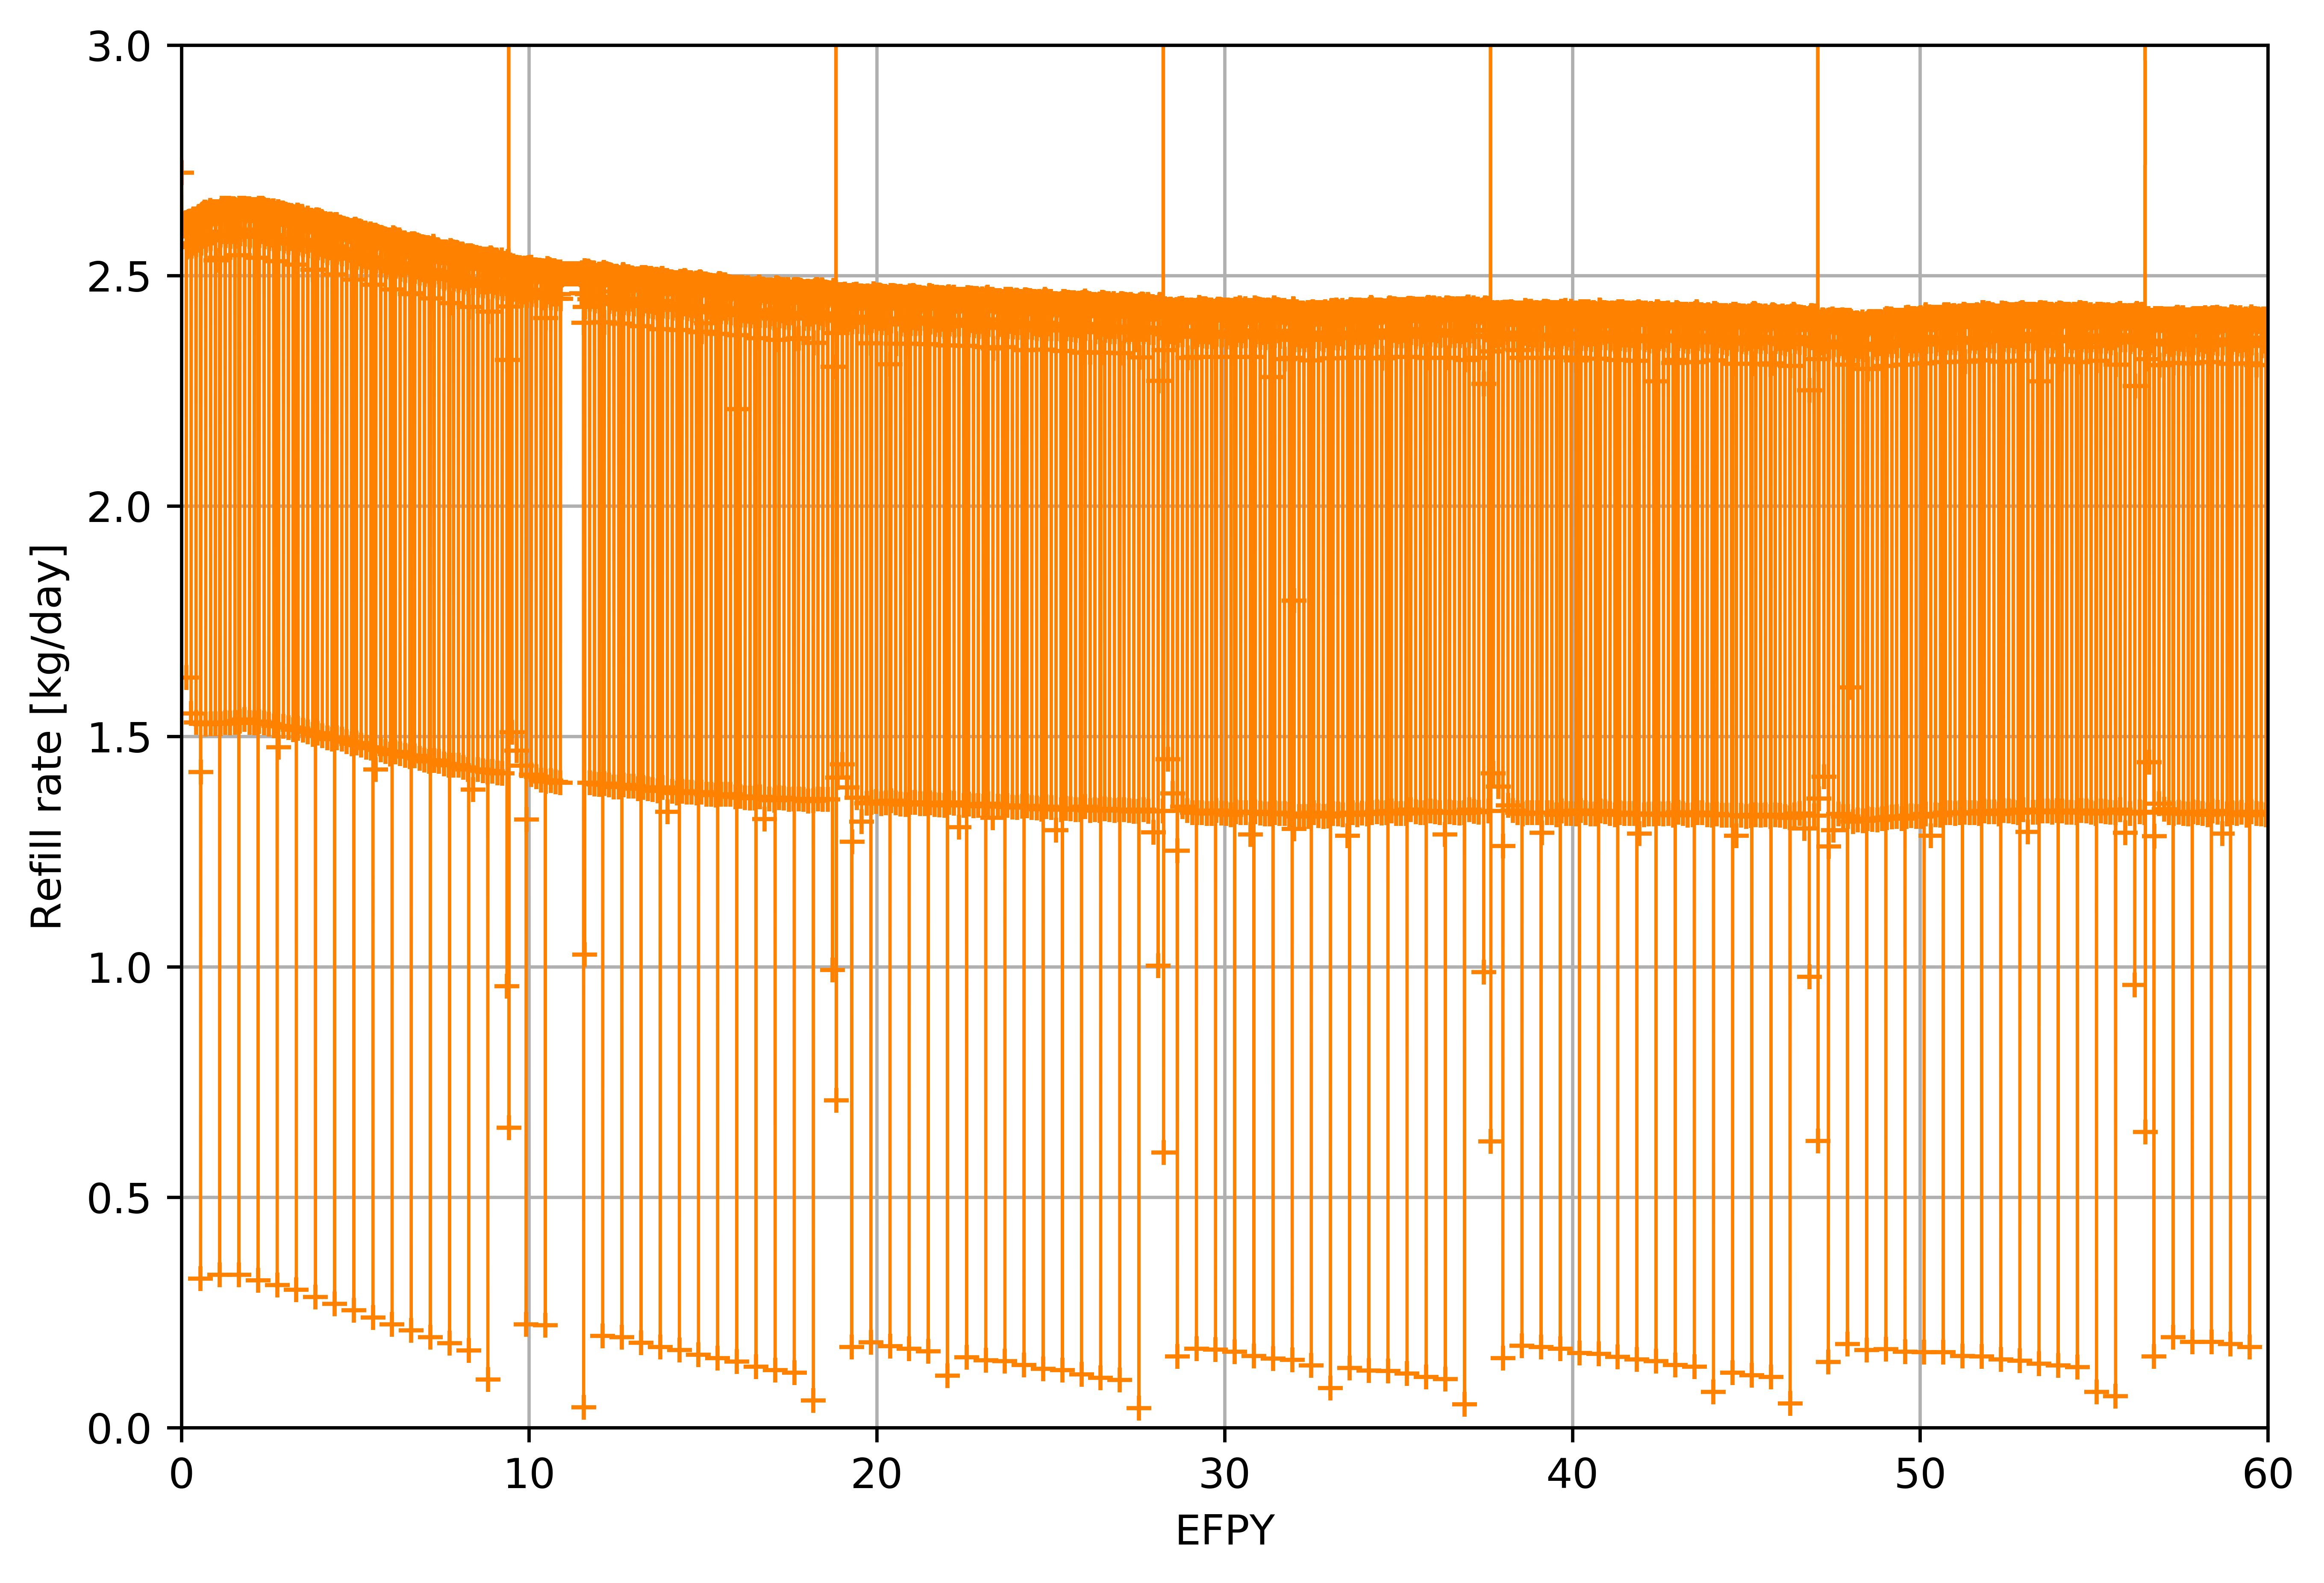
\includegraphics[width=\textwidth]{ch3/th_refill_rate.png} 
	\caption{$^{232}$Th feed rate over 60 years of the \gls{MSBR} operation 
	(reproduced from Rykhlevskii \emph{et al.} 
	\cite{rykhlevskii_modeling_2019}).}
	\label{fig:th_refill}
\end{figure}
\begin{figure}[ht!] % replace 't' with 'b' to force it to \centering
	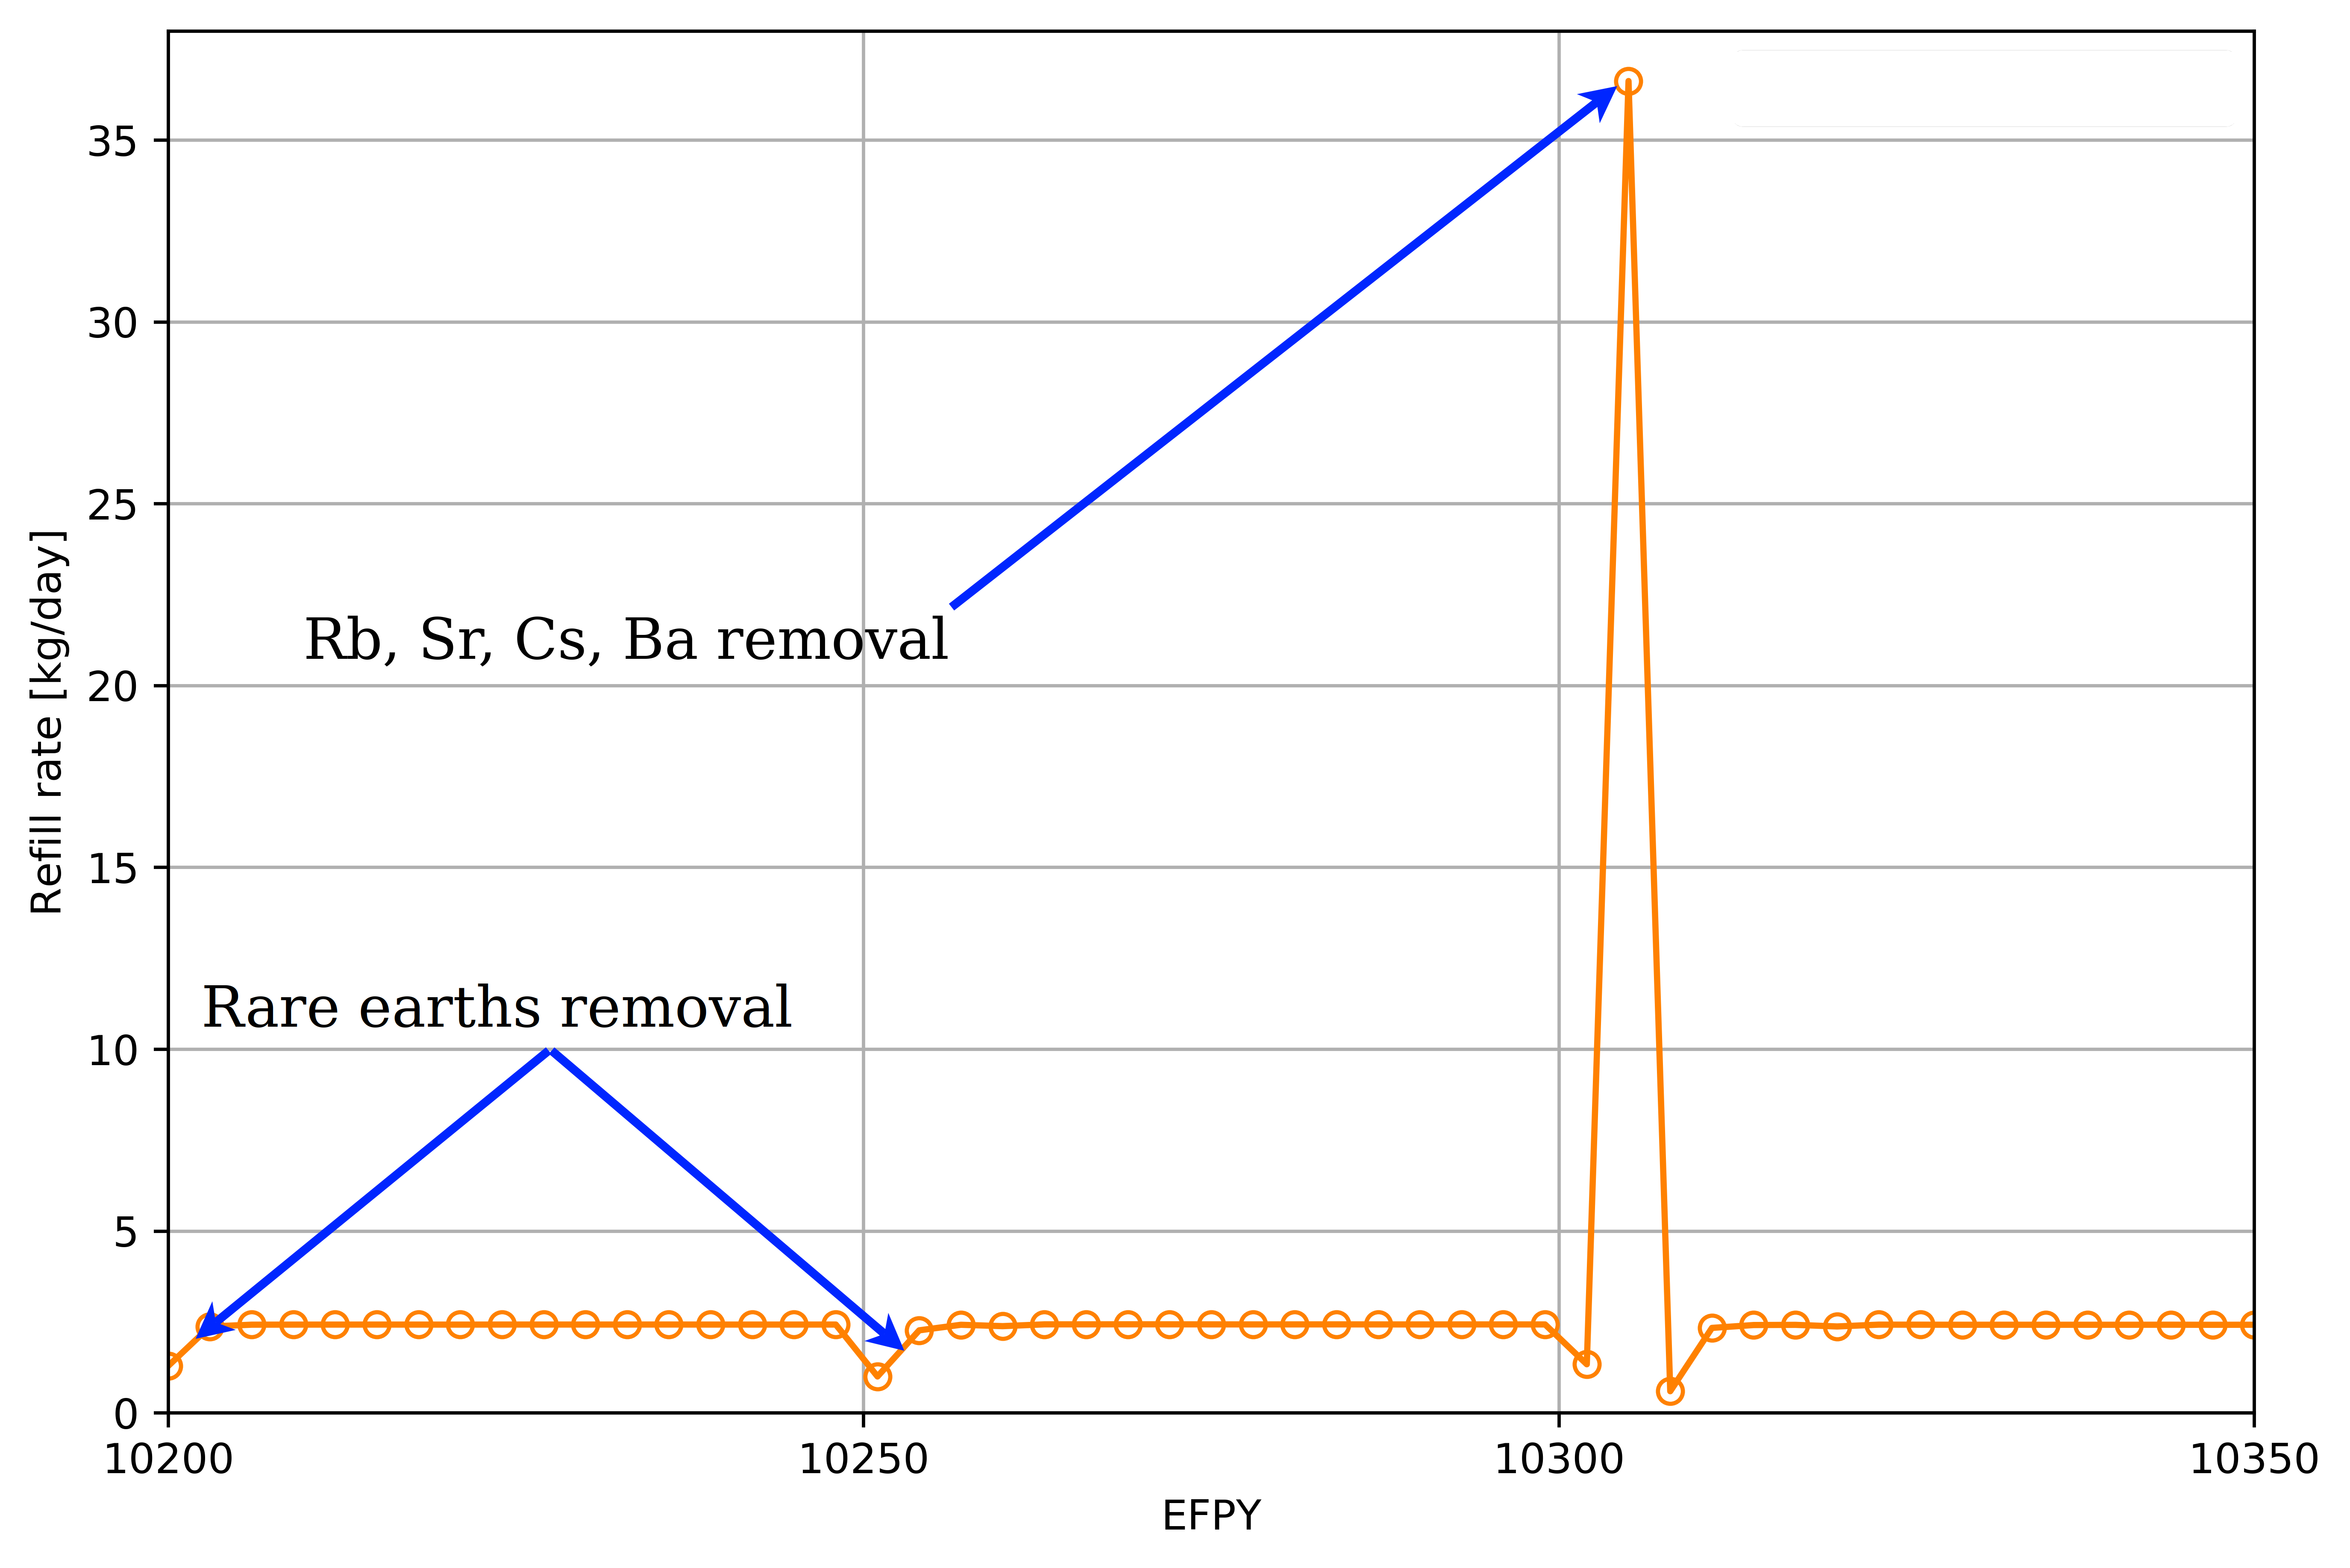
\includegraphics[width=\textwidth]{ch3/th_refill_rate_zoomed.png} 
	\caption{Zoomed $^{232}$Th feed rate for a 150-EFPD time interval 
	(reproduced from Rykhlevskii \emph{et al.} 
	\cite{rykhlevskii_modeling_2019}).}
	\label{fig:th_refill_zoomed}
\end{figure}

The average thorium feed rate increases during the first 500 days of operation 
and steadily decreases due to spectrum hardening and accumulation of absorbers 
in the core. As a result, the average $^{232}$Th feed rate over 60 years of 
operation is about 2.40 kg/day. This thorium consumption rate is in good 
agreement with a recent online reprocessing study by \gls{ORNL}  
\cite{betzler_molten_2017}. At equilibrium, the thorium feed rate is 
determined by the reactor power, the energy released per fission, and the 
neutron energy spectrum.


\section{Operational and safety parameters evolution}
In Section~\ref{sec:equilibrium_search}, we reported how fuel salt composition 
changes during \gls{MSBR} operation. The number density of the most 
important heavy isotopes, $^{233}$U and $^{232}$Th, was stable while 
transitioning from startup to equilibrium composition  
(Figure~\ref{fig:adens_eq}). At the same time, a number of different 
actinides is being produced in the reactor core. Most of these nuclides 
($^{234}$U, $^{239}$Pu, $^{241}$Pu) have a much larger absorption cross 
section than $^{233}$U and $^{232}$Th loaded initially into the core, which 
causes significant neutron energy spectrum hardening. In the current section, 
we analyze how such neutron spectrum shift affects major operation and safety 
parameters such as temperature coefficients of reactivity and reactivity worth 
of the control rods. 

\subsection{Temperature coefficient of reactivity}
Table~\ref{tab:tcoef} summarizes temperature effects on reactivity calculated 
in this work for both initial and equilibrium fuel compositions, compared 
to the original \gls{ORNL} report data \cite{robertson_conceptual_1971}. 
By propagating the $k_{eff}$  statistical error provided by Serpent, 
uncertainty for each temperature coefficient was obtained and appears in 
Table~\ref{tab:tcoef}. Other sources of uncertainty are neglected, such as 
cross section measurement error and approximations inherent in the equations 
of state, providing both the salt and graphite density dependence on 
temperature. The main physical principle underlying the reactor temperature 
feedback is an expansion of heated material. If the fuel salt temperature 
increases, the density of the salt decreases; at the same time, the total 
volume of fuel salt in the core remains constant because the graphite bounds 
it. If the graphite temperature increases, the density of graphite 
decreases, creating additional space for fuel salt. To determine the 
temperature coefficients, the cross section temperatures for the fuel and 
moderator were changed from 900K to 1000K. Three different cases were 
considered:
\begin{enumerate}[itemsep=1pt,parsep=2pt]
	\item Temperature of fuel salt rising from 900K to 1000K.
	\item Temperature of graphite rising from 900K to 1000K.
	\item Whole reactor temperature rising from 900K to 1000K.
\end{enumerate}
%%%%%%%%%%%%%%%%%%%%%%%%%%%%%%%%%%%%%%%%
\begin{table}[ht!]
	\caption{Temperature coefficients of reactivity for the initial and 
	equilibrium states (reproduced from Rykhlevskii \emph{et al.} 
		\cite{rykhlevskii_modeling_2019}).}
	\begin{tabularx}{\textwidth}{ p{0.3\textwidth} R R R } \hline
		Reactivity coefficient   & Initial & Equilibrium  &  Reference
		\cite{robertson_conceptual_1971}                             \\ 
		& [pcm/K]         &  [pcm/K]        & (initial) [pcm/K] 
		\tabularnewline  \hline
		Doppler in fuel salt                    & $-4.73\pm0.038$ & 
		$-4.69\pm0.038$ & $-4.37$  \tabularnewline
		Fuel salt density                       & $+1.21\pm0.038$ & 
		$+1.66\pm0.038$ & $+1.09$  \tabularnewline
		Total fuel salt                         & $-3.42\pm0.038$ & 
		$-2.91\pm0.038$ & $-3.22$  \tabularnewline \hline
		Graphite spectral shift                 & $+1.56\pm0.038$ & 
		$+1.27\pm0.038$ &          \tabularnewline
		Graphite density                        & $+0.14\pm0.038$ & 
		$+0.23\pm0.038$ &          \tabularnewline
		Total moderator (graphite)              & $+1.69\pm0.038$ & 
		$+1.35\pm0.038$ & $+2.35$  \tabularnewline \hline
		Total core                              & $-1.64\pm0.038$ & 
		$-1.58\pm0.038$ & $-0.87$  \tabularnewline \hline
	\end{tabularx}
	\label{tab:tcoef}
\end{table}
%%%%%%%%%%%%%%%%%%%%%%%%%%%%%%%%%%%%%%%%%%%%%%%%%%%%%%%%%%%%%%%%%%%%%%%%%%%%%%%%
In the first case, changes in the fuel temperature only impact fuel density. 
In this case, the geometry is unchanged because the fuel is a liquid. However, 
if the moderator heats up, both the density and the geometry change due to 
the thermal expansion of the solid graphite blocks and reflector. Accordingly, 
the new graphite density was calculated using a linear temperature expansion 
coefficient of 1.3$\times10^{-6}$K$^{-1}$ \cite{robertson_conceptual_1971}. A 
new geometry input for Serpent, which takes into account the displacement of 
graphite surfaces, was created based on this information. For calculation of 
displacement, it was assumed that the interface between the graphite reflector 
and vessel is immobile and the vessel temperature is constant. This 
is the most reasonable assumption for the short-term reactivity effects 
because inlet salt cools the graphite reflector and the inner surface of the 
vessel.

The fuel temperature coefficient (FTC) is negative for both initial and 
equilibrium fuel compositions due to thermal Doppler broadening of the 
resonance capture cross sections in the thorium. A small positive effect of 
fuel density on reactivity increases from $+1.21$ pcm/K at reactor startup to 
$+1.66$ pcm/K for equilibrium fuel composition, which has a negative effect on 
FTC magnitude during the reactor operation; this is in good agreement with 
earlier research \cite{robertson_conceptual_1971,park_whole_2015}. The 
moderator temperature coefficient (MTC) is positive for the startup 
composition and decreases during reactor operation because of spectrum 
hardening with fuel depletion. Finally, the total temperature coefficient of 
reactivity is negative for both cases but decreases in magnitude during 
reactor operation due to spectral shift. In summary, even after 20 years of 
operation, the total temperature coefficient of reactivity is relatively large 
and negative during reactor operation (comparing with conventional PWR which 
has temperature coefficient about -1.71 pcm/$^\circ$F $\approx$ -3.08 pcm/K 
\cite{forget_integral_2018}), despite positive MTC, and affords excellent 
reactor stability and control.

\subsection{Reactivity control system rod worth}
Table~\ref{tab:rod_worth} summarizes the reactivity control system worth. 
During normal operation, the control (graphite) rods are fully inserted, and 
the safety (B$_4$C) rods are fully withdrawn. To insert negative reactivity 
into the core, the graphite rods are gradually withdrawn from the core. In an 
accident, the safety rods would be dropped down into the core. The integral 
rod worths were calculated for various positions to separately estimate the 
worth of the control rods\footnote{In 
\cite{robertson_conceptual_1971}, the graphite rods are referred to as 
``control'' rods.}, the safety rods, and the whole reactivity control 
system. Control rod integral worth is approximately 28 cents and stays almost 
constant during reactor operation. The safety rod integral worth decreases by  
16.2\% during 20 years of operation because of neutron spectrum hardening and 
absorber accumulation in proximity to reactivity control system rods. This 
16\% decline in control system worth must be taken into account in \gls{MSBR} 
accident analysis and safety justification.
%%%%%%%%%%%%%%%%%%%%%%%%%%%%%%%%%%%%%%%%
\begin{table}[ht!]
	\caption{Control system rod worth for the initial and equilibrium fuel 
		compositions (reproduced from Rykhlevskii \emph{et al.} 
		\cite{rykhlevskii_modeling_2019}).}
	\begin{tabularx}{\textwidth}{ p{0.5\textwidth}  R  R } \hline
		Reactivity parameter  &  Initial[\cent]    &  Equilibrium[\cent]  \\ 
		\hline
		Control (graphite) rod integral worth               & $\ 28.2\pm0.8$    
		& $\ 
		29.0\pm0.8$ \\ Safety rod integral worth                  & 
		$251.8\pm0.8$    & $211.0\pm0.8$  \\
		Total reactivity control system worth               & $505.8\pm0.7$    
		& 
		$424.9\pm0.8$ \\ \hline
	\end{tabularx}
	\label{tab:rod_worth}
\end{table}
%%%%%%%%%%%%%%%%%%%%%%%%%%%%%%%%%%%%%%%%%%%%%%%%%%%%%%%%%%%%%%%%%%%%%%%%%%%%%%%%

\subsection{Six Factor Analysis}
The effective multiplication factor can be expressed using the following 
formula:
\begin{align}
k_{eff} &=  \eta f p \epsilon P_f P_t
\intertext{where}
\eta     &= \mbox{neutron reproduction factor $[-]$}  \nonumber \\
f        &= \mbox{thermal utilization factor $[-]$}   \nonumber \\
p        &= \mbox{resonance escape probability $[-]$} \nonumber \\
\epsilon &= \mbox{fast fission factor $[-]$}          \nonumber \\
P_f      &= \mbox{fast non-leakage probability $[-]$} \nonumber \\
P_t      &= \mbox{thermal non-leakage probability $[-]$.} \nonumber
\end{align}

Table~\ref{tab:six_factor} summarizes the six factors for both the initial and 
equilibrium fuel salt compositions. Using Serpent and SaltProc, these factors 
and their statistical uncertainties have been calculated for both the initial 
and equilibrium fuel salt compositions (see Table~\ref{tab:msbr_tab}). The 
fast and thermal non-leakage probabilities remain constant despite the 
evolving neutron spectrum during operation. In contrast, the neutron 
reproduction factor ($\eta$), resonance escape probability ($p$), and fast 
fission factor ($\epsilon$) are considerably different between startup and 
equilibrium. As indicated in Figure~\ref{fig:spectrum}, the neutron spectrum 
is softer at the beginning of reactor life. Neutron spectrum hardening causes 
the fast fission factor to increase through the core lifetime; the opposite is 
true for the resonance escape probability. Finally, the neutron reproduction 
factor decreases during reactor operation due to the accumulation of fissile 
plutonium isotopes.
%%%%%%%%%%%%%%%%%%%%%%%%%%%%%%%%%%%%%%%%
\begin{table}[hb!]
	\caption{Six factors for the full-core \gls{MSBR} model for the initial 
	and equilibrium fuel compositions (reproduced from Rykhlevskii \emph{et 
		al.} \cite{rykhlevskii_modeling_2019}).}
	\begin{tabularx}{\textwidth}{ p{0.5\textwidth}  R  R } \hline
		Factor  & Initial      & Equilibrium   \\ \hline
		Neutron reproduction factor ($\eta$)     & $1.3960\pm.000052$     & 
		$1.3778\pm.00005$ \\ Thermal utilization factor (f)           & 
		$0.9670\pm.000011$     & $0.9706\pm.00001$ \\
		Resonance escape probability (p)         & $0.6044\pm.000039$     & 
		$0.5761\pm.00004$ \\
		Fast fission factor ($\epsilon$)         & $1.3421\pm.000040$     & 
		$1.3609\pm.00004$ \\
		Fast non-leakage probability (P$_f$)     & $0.9999\pm.000004$     & 
		$0.9999\pm.000004$ \\
		Thermal non-leakage probability (P$_t$)  & $0.9894\pm.000005$     & 
		$0.9912\pm.00005$ \\ \hline
	\end{tabularx}
	\label{tab:six_factor}
\end{table}

\section{Benefits of fission products removal}
To investigate how online fuel salt processing described in Chapter 2 affects 
the reactor performance, the separate effect of each poison group removal 
was studied in this section.

\subsection{The effect of removing fission products from the fuel salt}
Loading the initial fuel salt composition into the \gls{MSBR} core leads to a 
supercritical configuration (Figure~\ref{fig:fp_removal}). After reactor 
startup, the effective multiplication factor for the case with volatile gases 
and noble metals removal is approximately 7500 pcm  higher than for the case 
without fission product removal. This significant impact on the reactor core 
lifetime is achieved due to the immediate removal (20 sec cycle time) and the 
high absorption cross sections of Xe, Kr, Mo, and other noble metals removed. 
The effect of rare earth element removal is significant in a few months after 
startup and reached approximately 5500 pcm after 10 years of operation. The 
rare earth elements were removed at a slower rate (50-day cycle time). 
Moreover, Figure~\ref{fig:fp_removal} demonstrates that batch-wise removal of 
strong absorbers every 3 days unnecessarily leads to fluctuation in results, 
but rare earth element removal every 50 days causes an approximately 600 pcm 
jump in reactivity.
\begin{figure}[ht!] % replace 't' with 'b' to force it to 
	\centering
	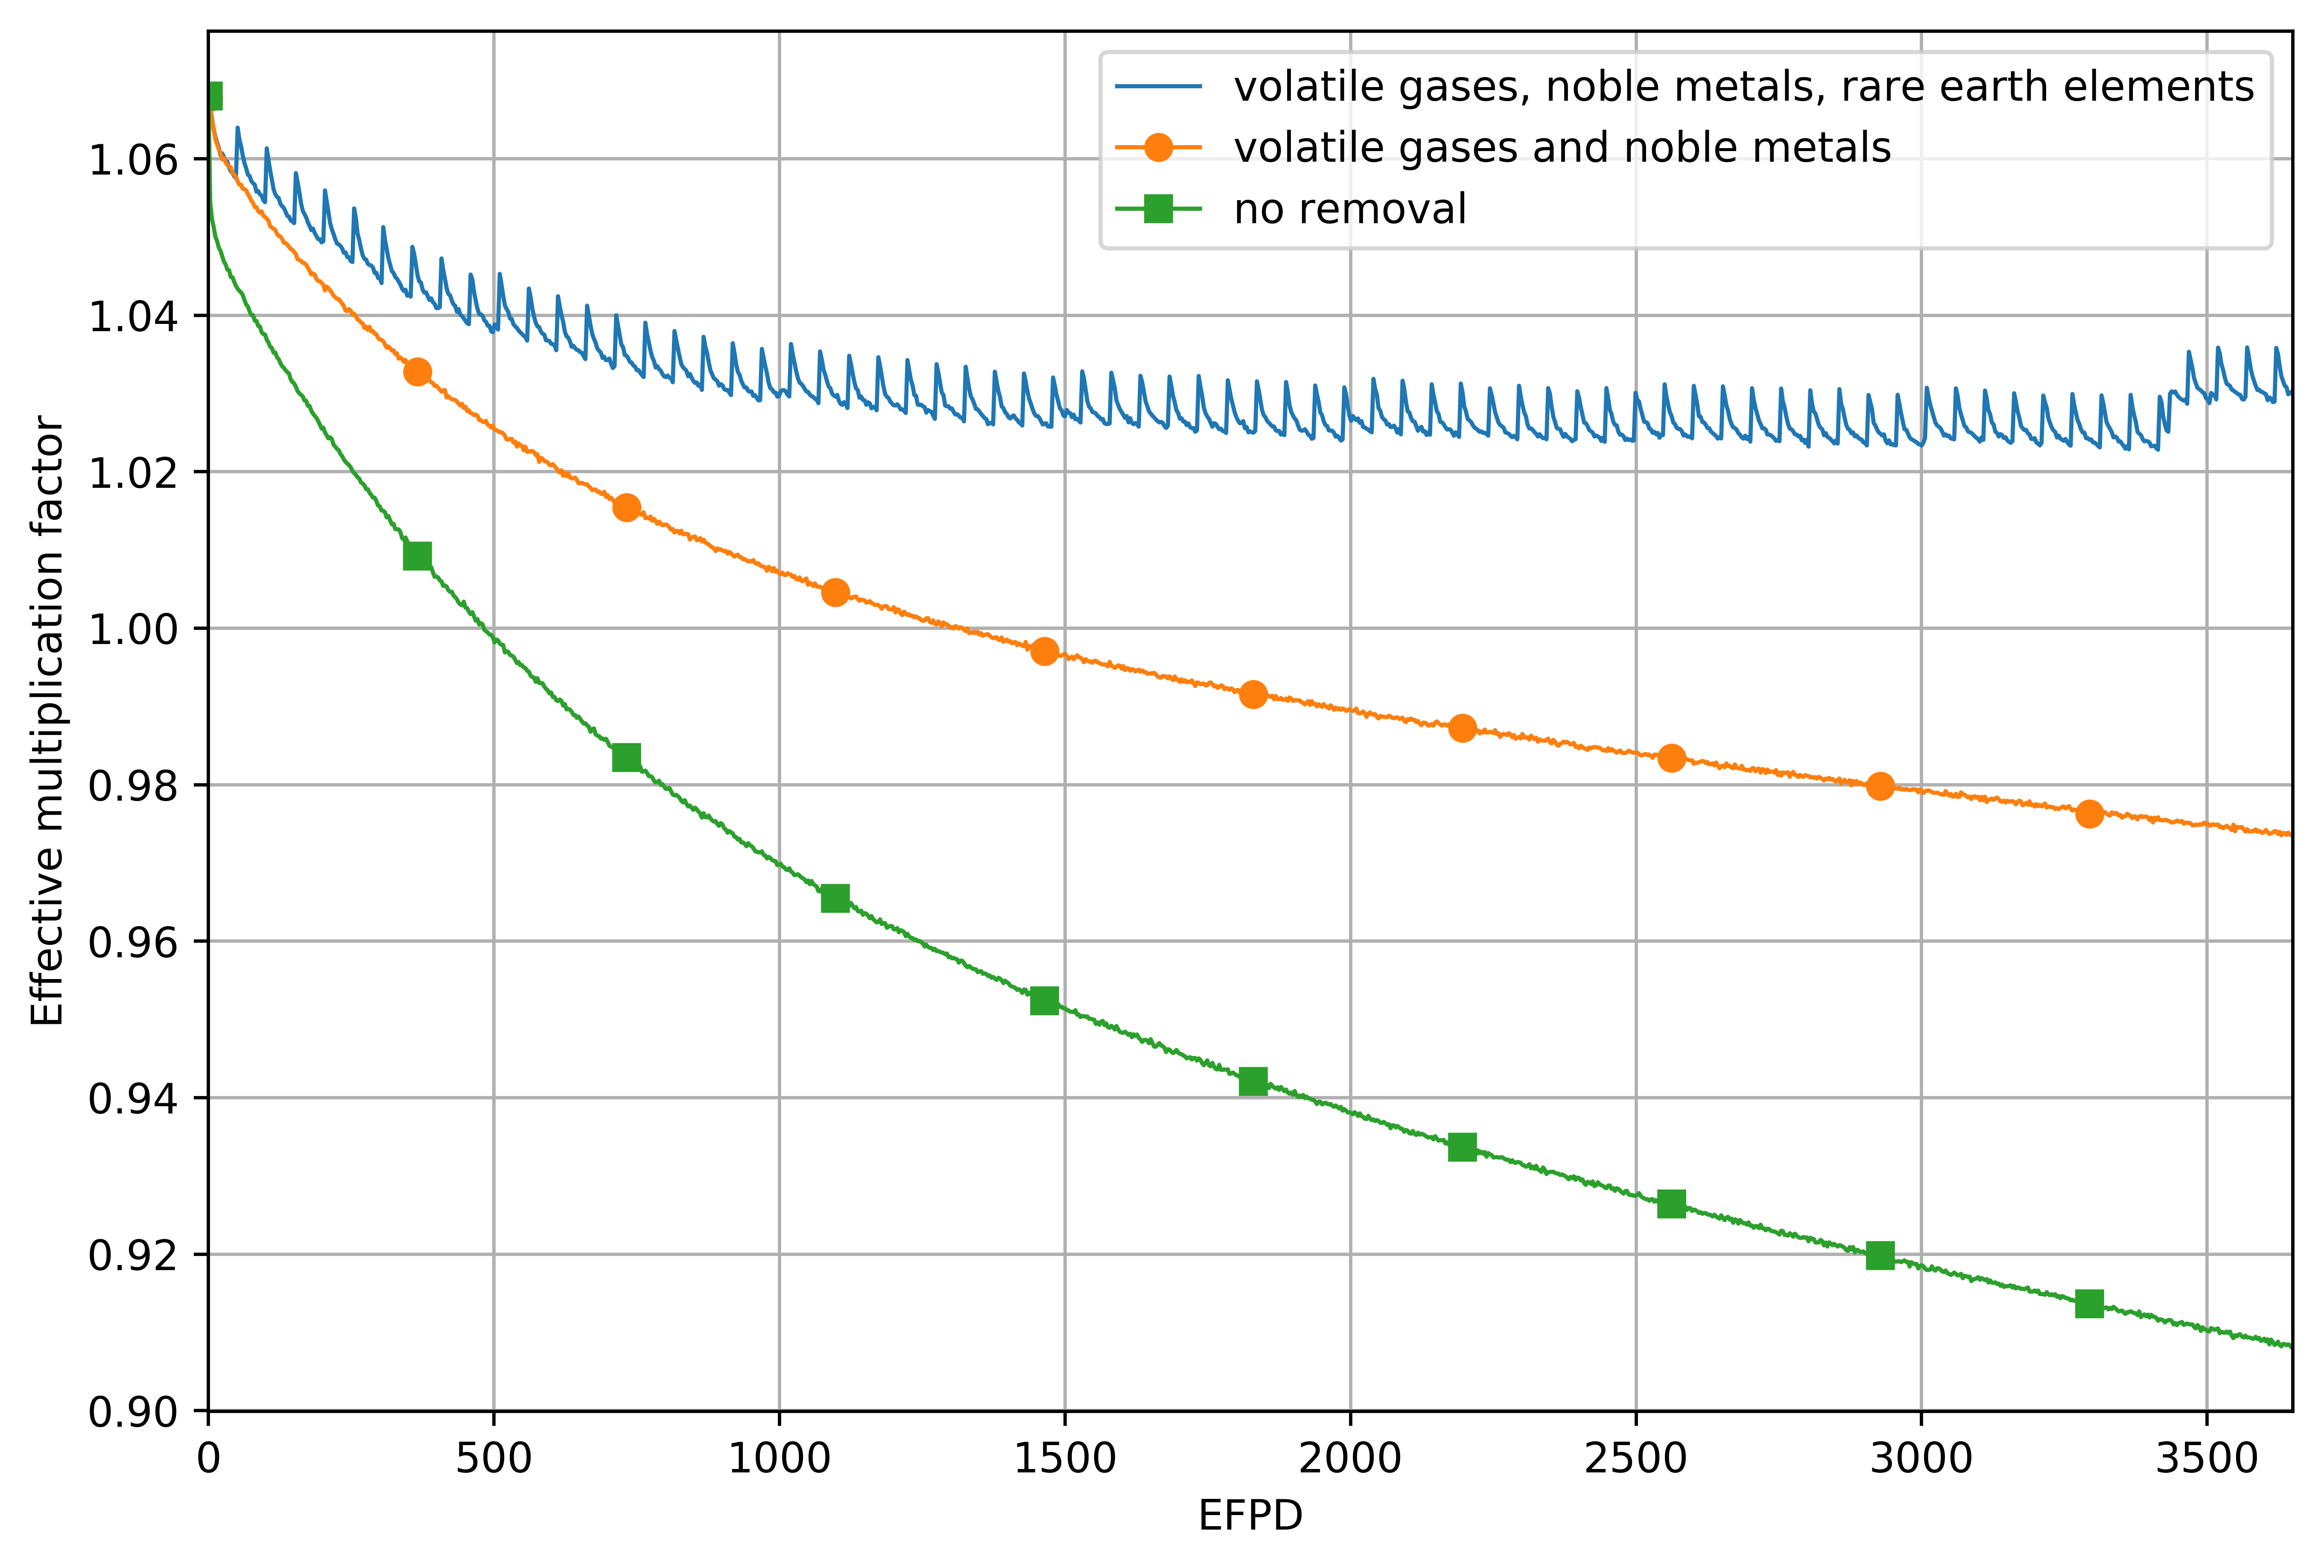
\includegraphics[width=\textwidth]{ch3/keff_rem_cases.png} 
	\caption{Calculated effective multiplication factor for the full-core 
		\gls{MSBR} model with the removal of various fission product groups 
		over 10 years of operation (reproduced from Rykhlevskii \emph{et al.} 
		\cite{rykhlevskii_modeling_2019}).}
	\label{fig:fp_removal}
\end{figure}

The effective multiplication factor of the core reduces gradually over 
operation time because the fissile material ($^{233}$U) continuously depletes 
from the fuel salt due to fission while fission products accumulate in the 
fuel salt simultaneously. Eventually, without fission products removal, the 
reactivity decreases to the subcritical state after approximately 500 and 
1300 days of operation for cases with no removal and volatile gases \& noble 
metals removal, respectively. The time when the simulated core becomes  
subcritical ($k_{eff}<$1.0 for full-core model) is called the core 
lifetime. Therefore, removing fission products provides significant 
neutronic benefits and enables a longer core lifetime.


\section{Concluding remarks}

This chapter introduces the first ever version of the open-source \gls{MSR} 
simulation package SaltProc v0.1. The main goal of this work has been to 
demonstrate SaltProc's capability to find the equilibrium fuel salt 
composition (the number densities of major isotopes vary by less than 1\% over 
several years). A secondary goal has been to compare predicted operational and 
safety parameters (e.g., neutron energy spectrum, power and breeding 
distribution, temperature coefficients of reactivity) of the \gls{MSBR} at 
startup and equilibrium states. A tertiary goal has been to demonstrate the 
benefits of continuous fission product removal for thermal \gls{MSR} design.

To achieve these goals, a full-core high-fidelity benchmark model of the 
\gls{MSBR} was created in Serpent 2. The full-core model was used instead of 
the simplified single-cell model \cite{betzler_molten_2017, 	
rykhlevskii_online_2017, betzler_fuel_2018} to precisely describe the 
two-region \gls{MSBR} concept design sufficiently to represent breeding in the 
outer core zone accurately. When running depletion calculations, the most 
critical fission products and $^{233}$Pa are removed, while fertile and  
fissile materials are added to the fuel salt every 3 days.  Meanwhile, the 
removal interval for the rare earths, volatile fluorides, and semi-noble 
metals was greater than one month (50 days), which caused significant 
$k_{eff}$  
fluctuation. 

The results in this chapter indicate that $k_{eff}$ slowly decreases from 
1.075 and reaches 1.02 at equilibrium after approximately 6 years of 
operation. At the same time, the concentrations of $^{233}$U, $^{232}$Th, 
$^{233}$Pa, and $^{232}$Pa stabilized after approximately 2500 days of 
operation. Particularly, $^{233}$U number density 
equilibrates\footnote{fluctuates less than 0.8\%} after 16 years of operation. 
Consequently, the core reaches the quasi-equilibrium state after 16 years of 
operation. However, a wide variety of actinides, including fissile isotopes 
(e.g., $^{233}$U and $^{239}$Pu) and non-fissile strong absorbers ($^{234}$U), 
continue accumulating in the core. 

Those actinides cause neutron energy spectrum hardening as the core  
approaches equilibrium. Moreover, the neutron energy spectrum in the central 
core region is much softer than in the outer core region due to the lower 
moderator-to-fuel ratio in the outer zone, and this distribution remains 
stable during reactor operation. Finally, the epithermal or thermal spectrum 
is needed to effectively breed $^{233}$U from $^{232}$Th because the radiative 
capture cross section of thorium-232 monotonically decreases from $10^{-10}$ 
MeV to $10^{-5}$ MeV. A harder spectrum in the outer core region tends to 
significantly increase resonance absorption in thorium and decrease the 
absorptions in fissile and structural materials. 

The spatial power distribution in the \gls{MSBR} shows that 98\% of the 
fission power is generated in the central zone I, and the neutron energy 
spectral shift has zero effect on the power distribution. The 
spatial distribution of neutron capture reaction rate for fertile $^{232}$Th, 
corresponding to breeding in the core, confirms that most of the breeding 
occurs in an outer, undermoderated, region of the \gls{MSBR} core. Finally, 
the average $^{232}$Th refill rate throughout 60 years of operation is 
approximately 2.40 kg/day or 100 g/GWh$_e$.

We compared the safety parameters at startup and state using the Serpent Monte 
Carlo code. The total temperature coefficient is large and negative at startup 
and equilibrium, but the magnitude decreases throughout reactor operation from 
$-3.10$ to $-0.94$ pcm/K as the spectrum hardens. The moderator temperature 
coefficient is positive and also decreases during fuel depletion. The 
reactivity control system efficiency analysis showed that the safety rod 
integral worth decreases by approximately 16.2\% over 16 years of operation, 
while the graphite rod integral worth remains constant. Therefore, neutron 
energy spectrum hardening during fuel salt depletion has an undesirable impact 
on \gls{MSBR} stability and controllability and should be taken into  
consideration in further analysis of transient accident scenarios.

Finally, we proved that the \gls{MSBR} core performance benefits from the 
removal of volatile gases, noble metals, and rare earths from the fuel salt. 
Immediate removal of volatile gases (e.g., xenon) and noble metals 
increased reactivity by approximately 7500 pcm over a 10-year timeframe. In 
contrast, the effect of relatively slower removal of rare earth elements 
(every 50 days cycle instead of 3 days) has less impact (5500 pcm) on the core 
reactivity after 10 years of operation. An additional study is needed to 
establish neutronic  and economic tradeoffs of removing each element.

This chapter's results also helped identify the main directions of SaltProc 
v0.1 improvement. Firstly, the poison removal efficiency is not ideal, as was 
discussed in Chapter 1; consequently, the user should be able to simulate the 
fuel salt reprocessing system using a variable, non-ideal extraction 
efficiency. Secondly, SaltProc v0.1 entirely removes elements with longer 
residence times (semi-noble metals, volatile fluorides, Rb, Sr, Cs, Ba, Eu) at 
the end of cycle time (e.g., 3435 days for rubidium) which causes significant  
jumps in $k_{eff}$ due to the removal of large batches of the poison at once. 
In SaltProc v1.0, this drawback has been eliminated by removing a fraction of 
the target element with longer residence time at each depletion step. In the 
following chapters, improved SaltProc v1.0 capabilities will be demonstrated.